\chapter{Application: Cardiac Mechanics}
%

\begin{figure}[ht]
\centering
\subfigure[]{%
		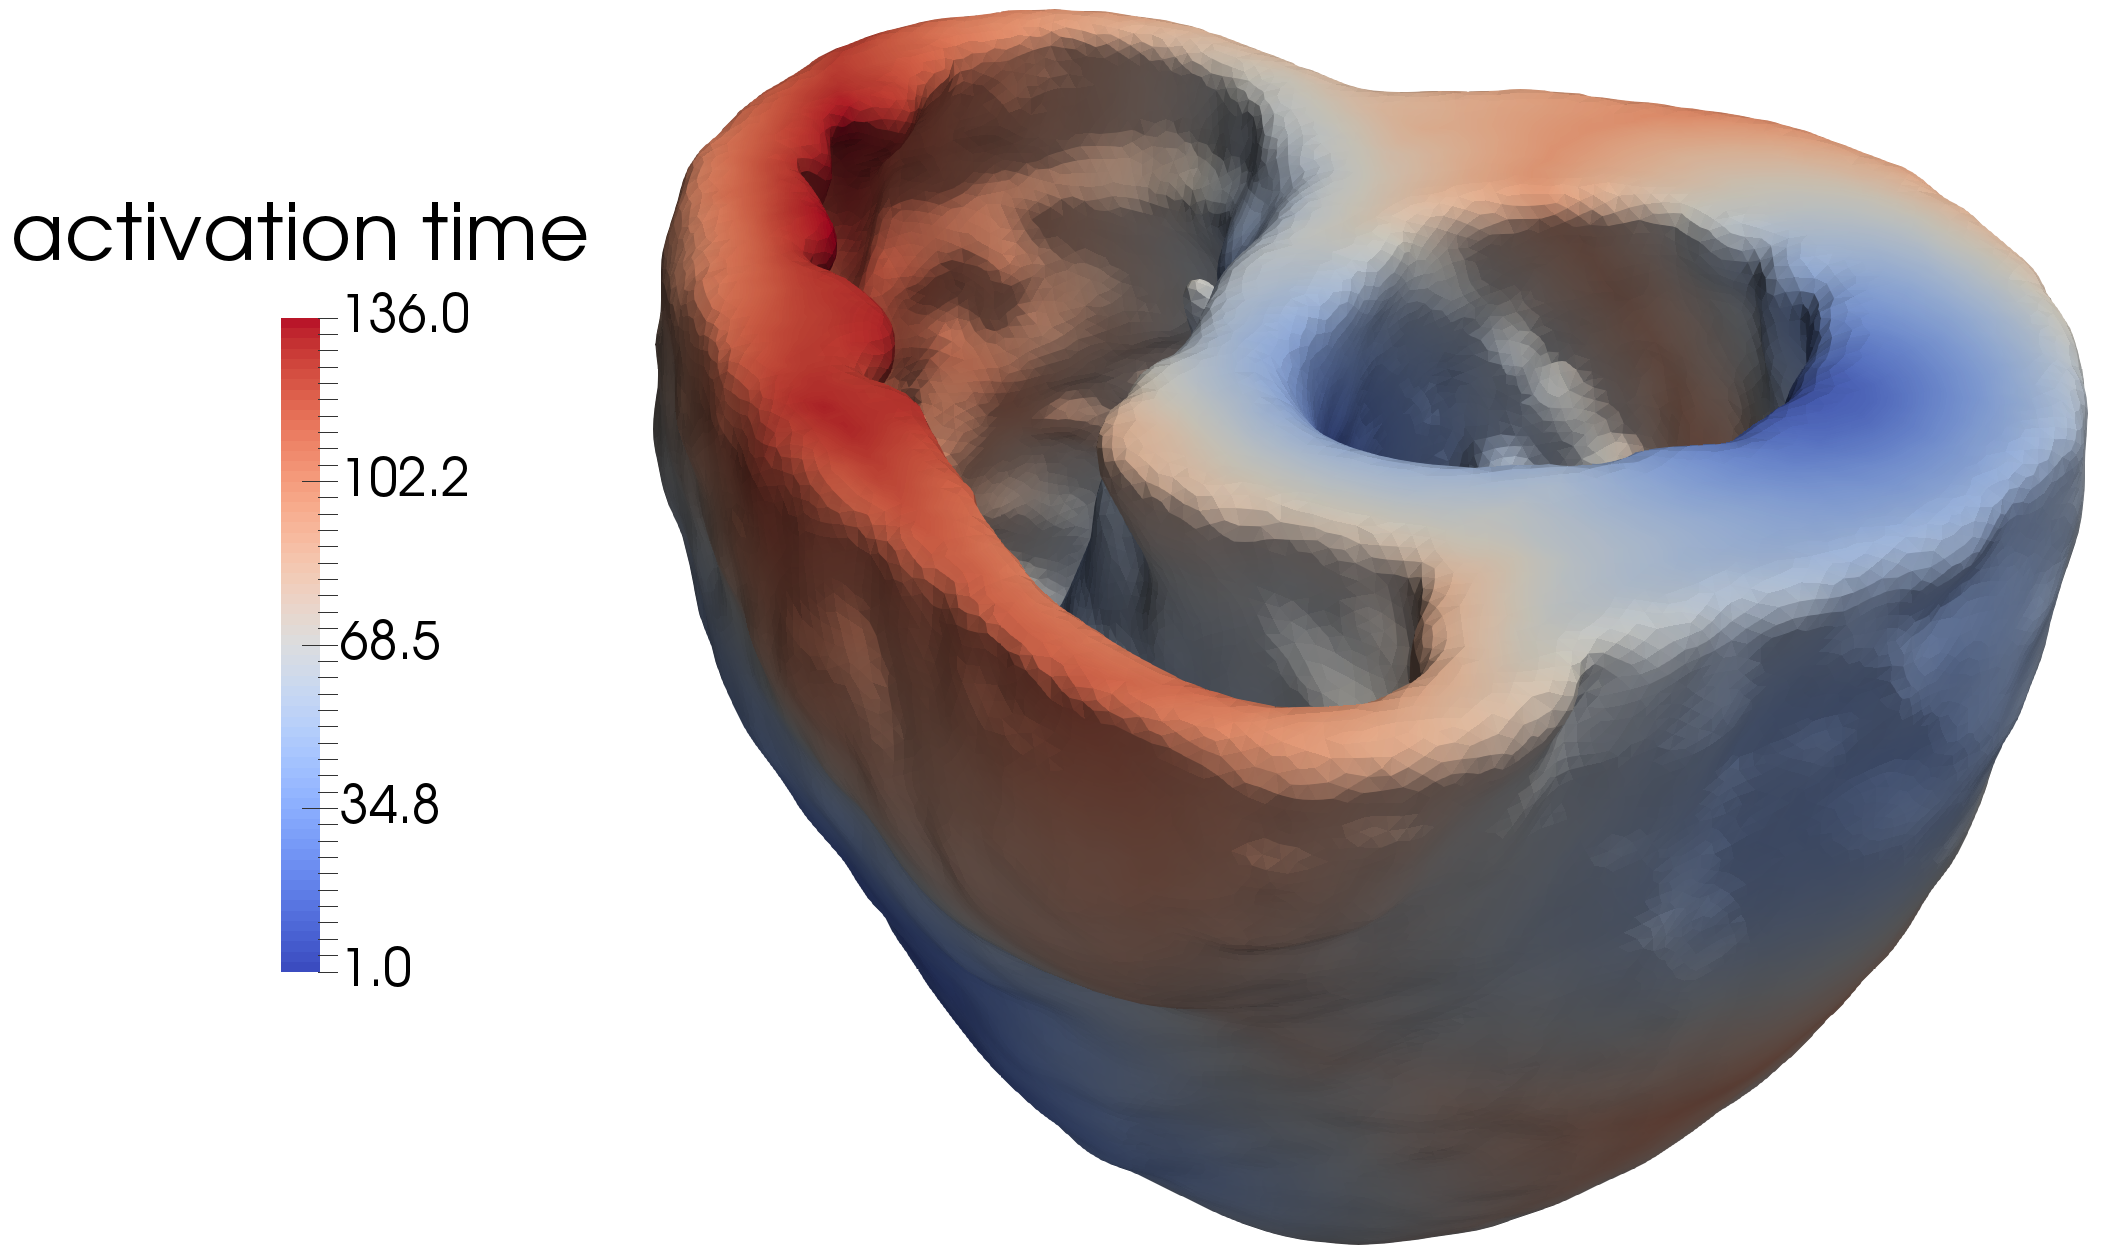
\includegraphics[scale=0.081]{media/4-cardioid/2-activationtime.png}
\label{fig:supp1}}
\subfigure[]{%
		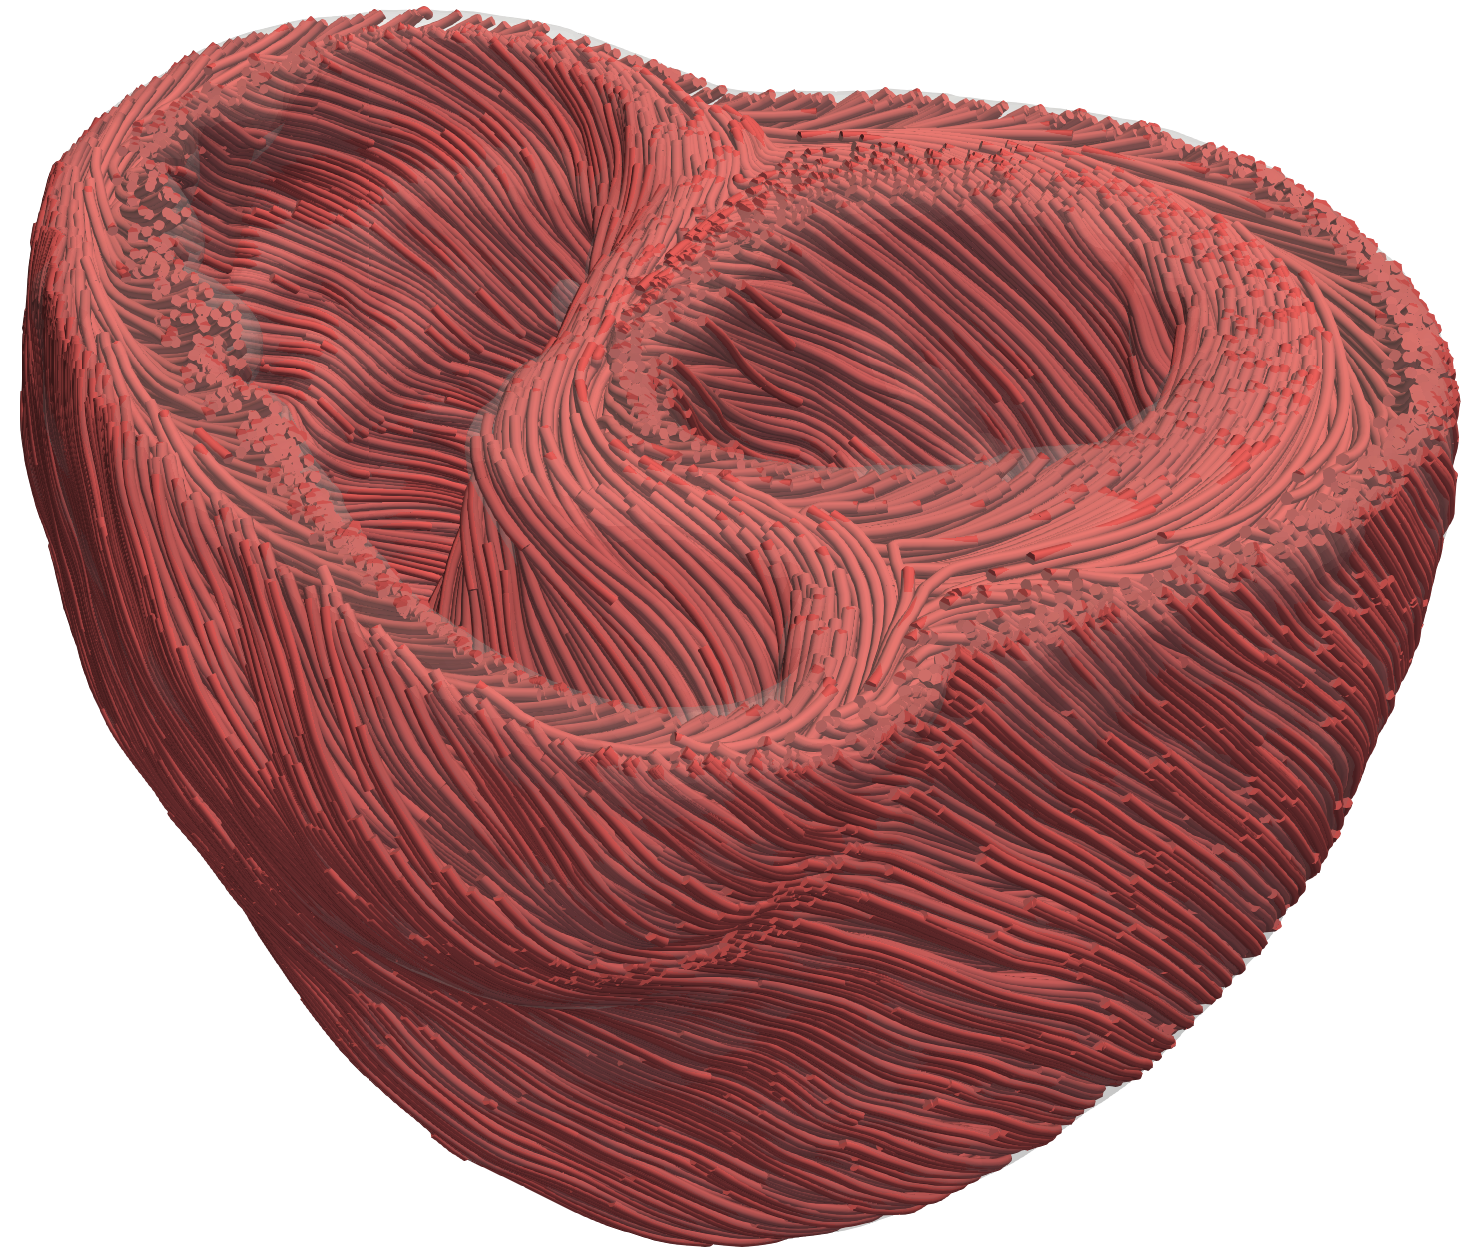
\includegraphics[scale=0.081]{media/4-cardioid/3-fibers.png}
\label{fig:supp2}}
\subfigure[]{%
		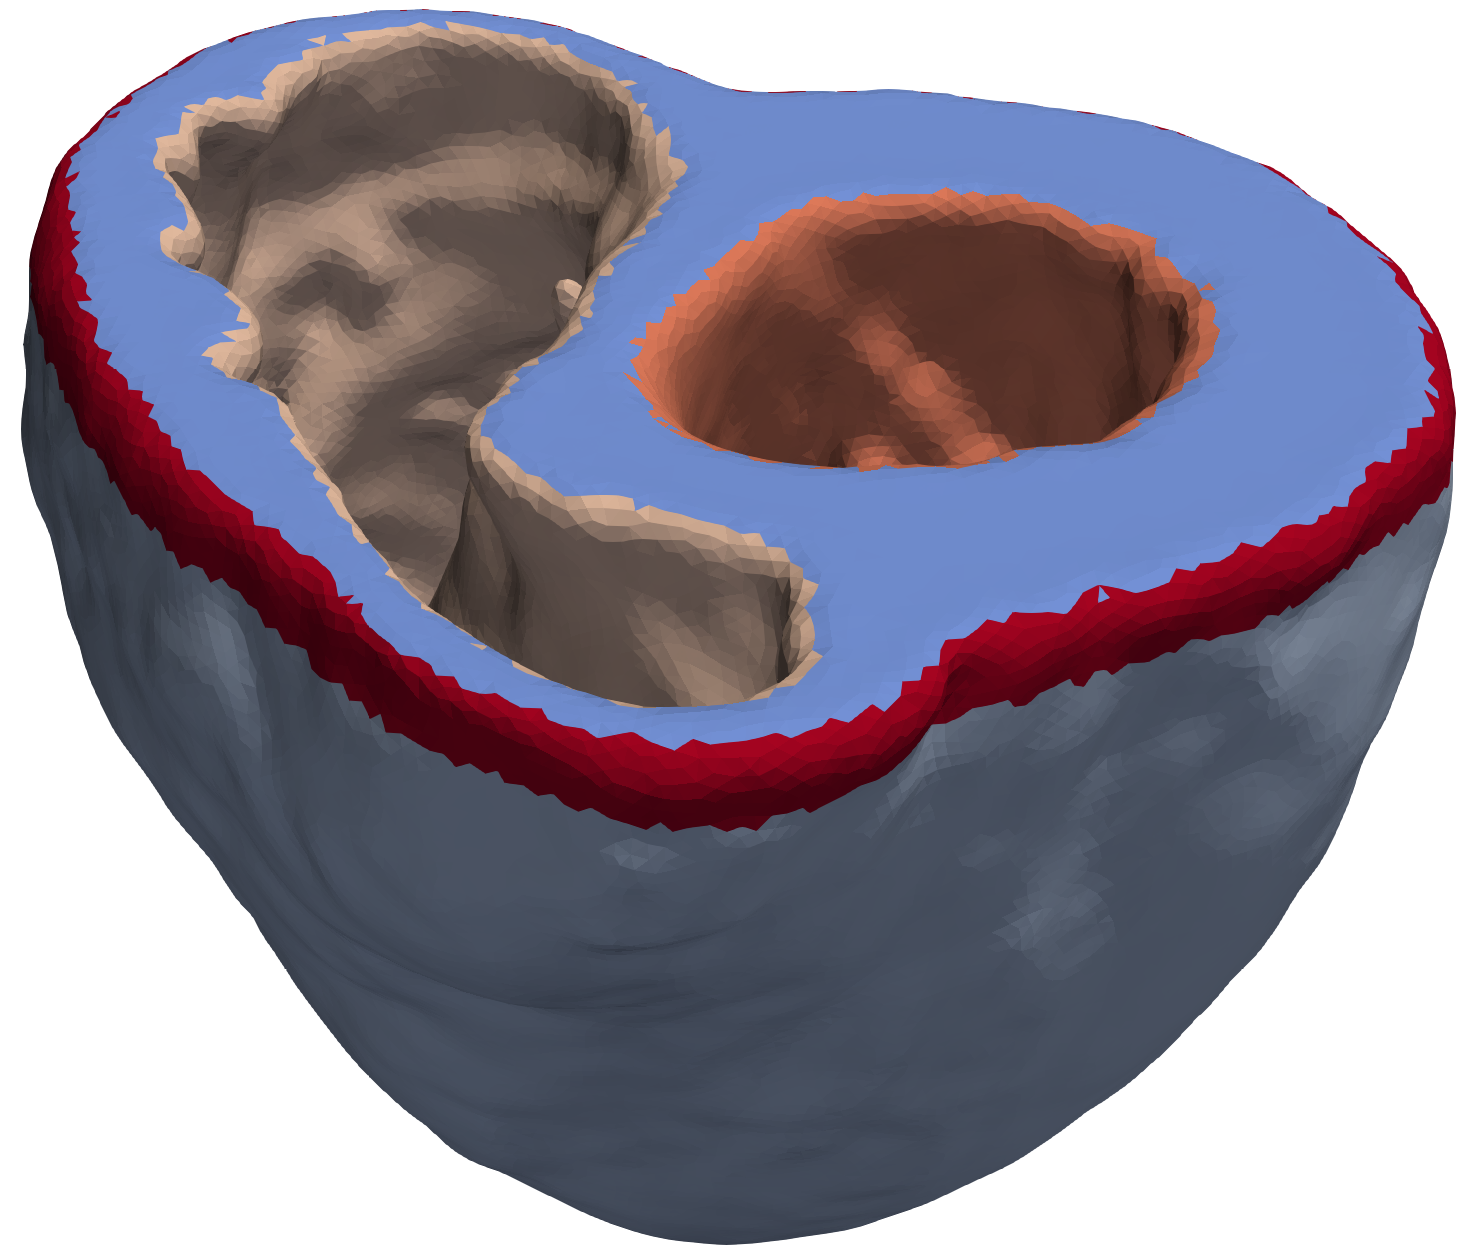
\includegraphics[scale=0.081]{media/4-cardioid/4-tagged.png}
\label{fig:supp3}}
%
\caption{Mechanics modeling considerations: (a) muscle fiber orientations, (b) electrical activation times, and c) surface tagging and prescription of corresponding boundary conditions.}
\label{fig:supp}
\end{figure}

\begin{figure}[ht]
\centering
\subfigure[]{%
		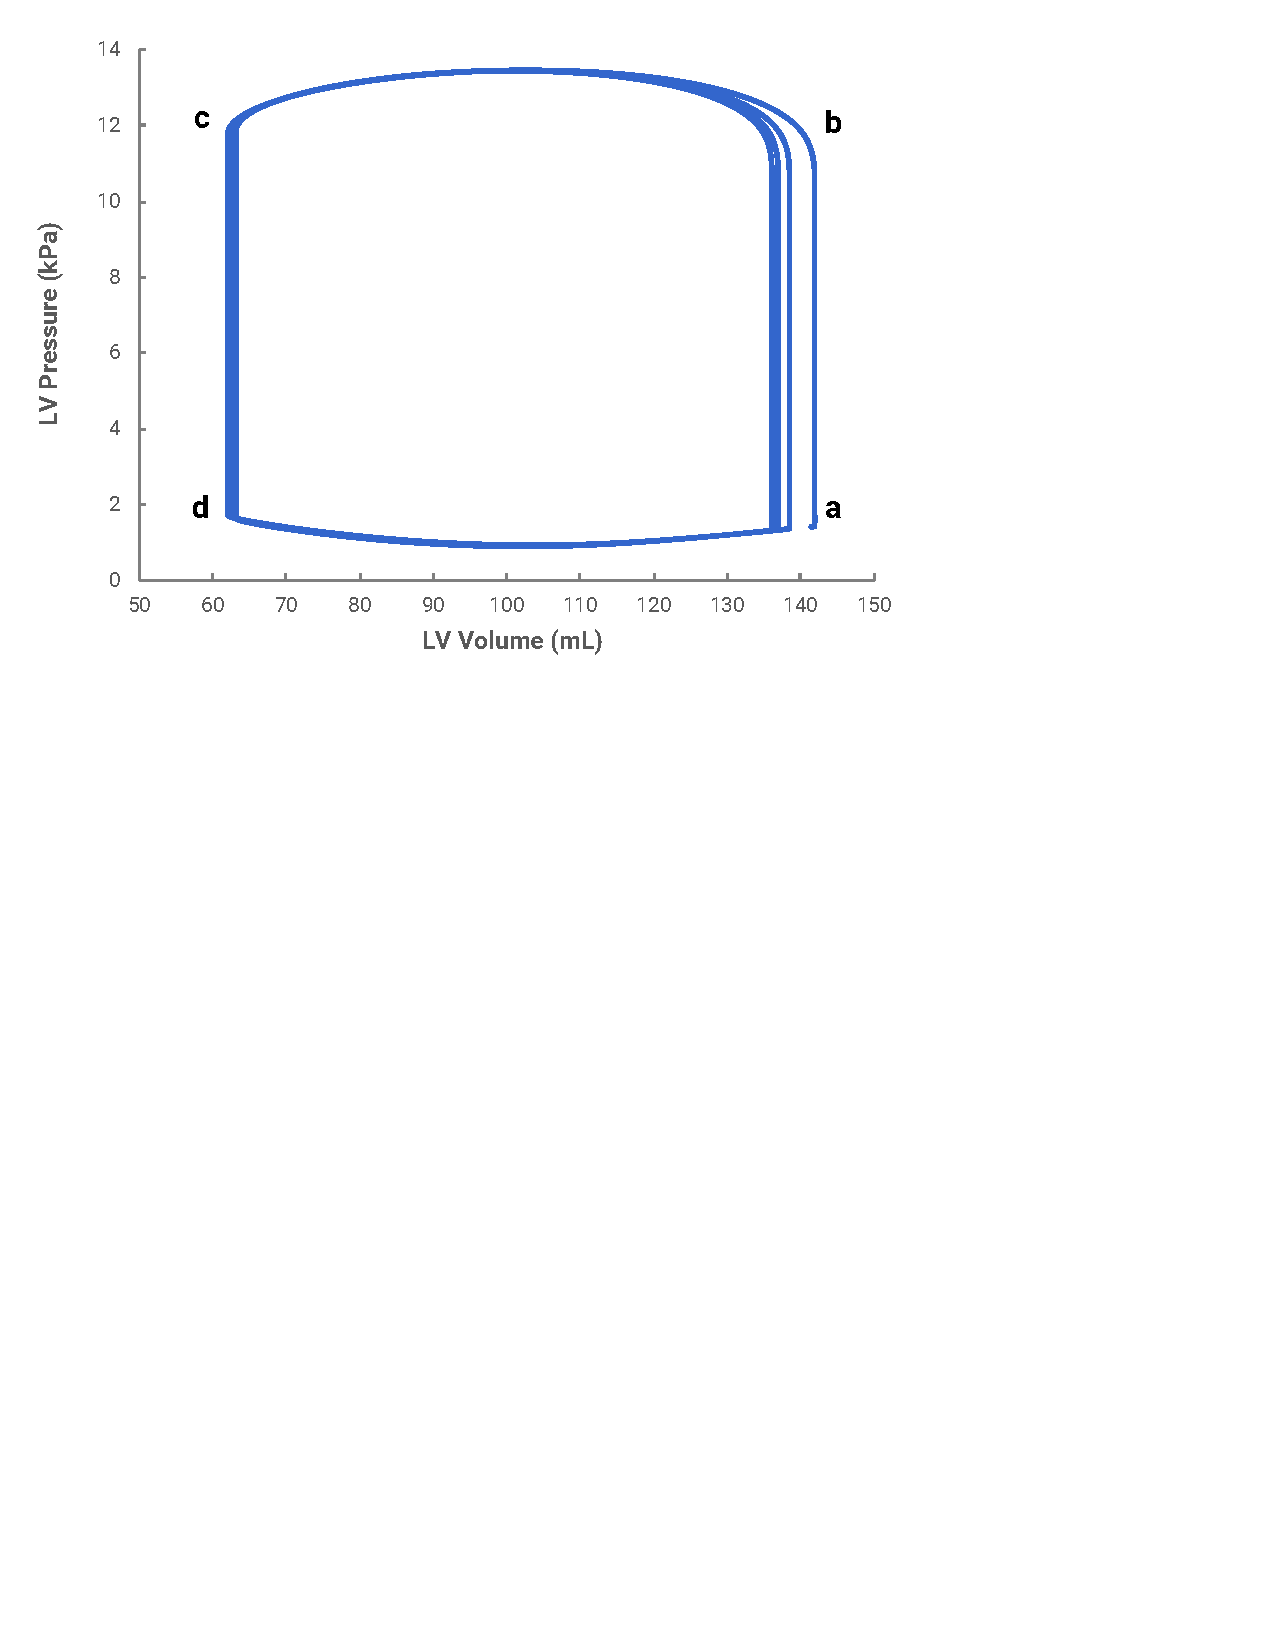
\includegraphics[scale=0.5]{media/4-cardioid/5-pv/pressure_volume-1.pdf}
\label{fig:pv1}}		
\subfigure[]{%
		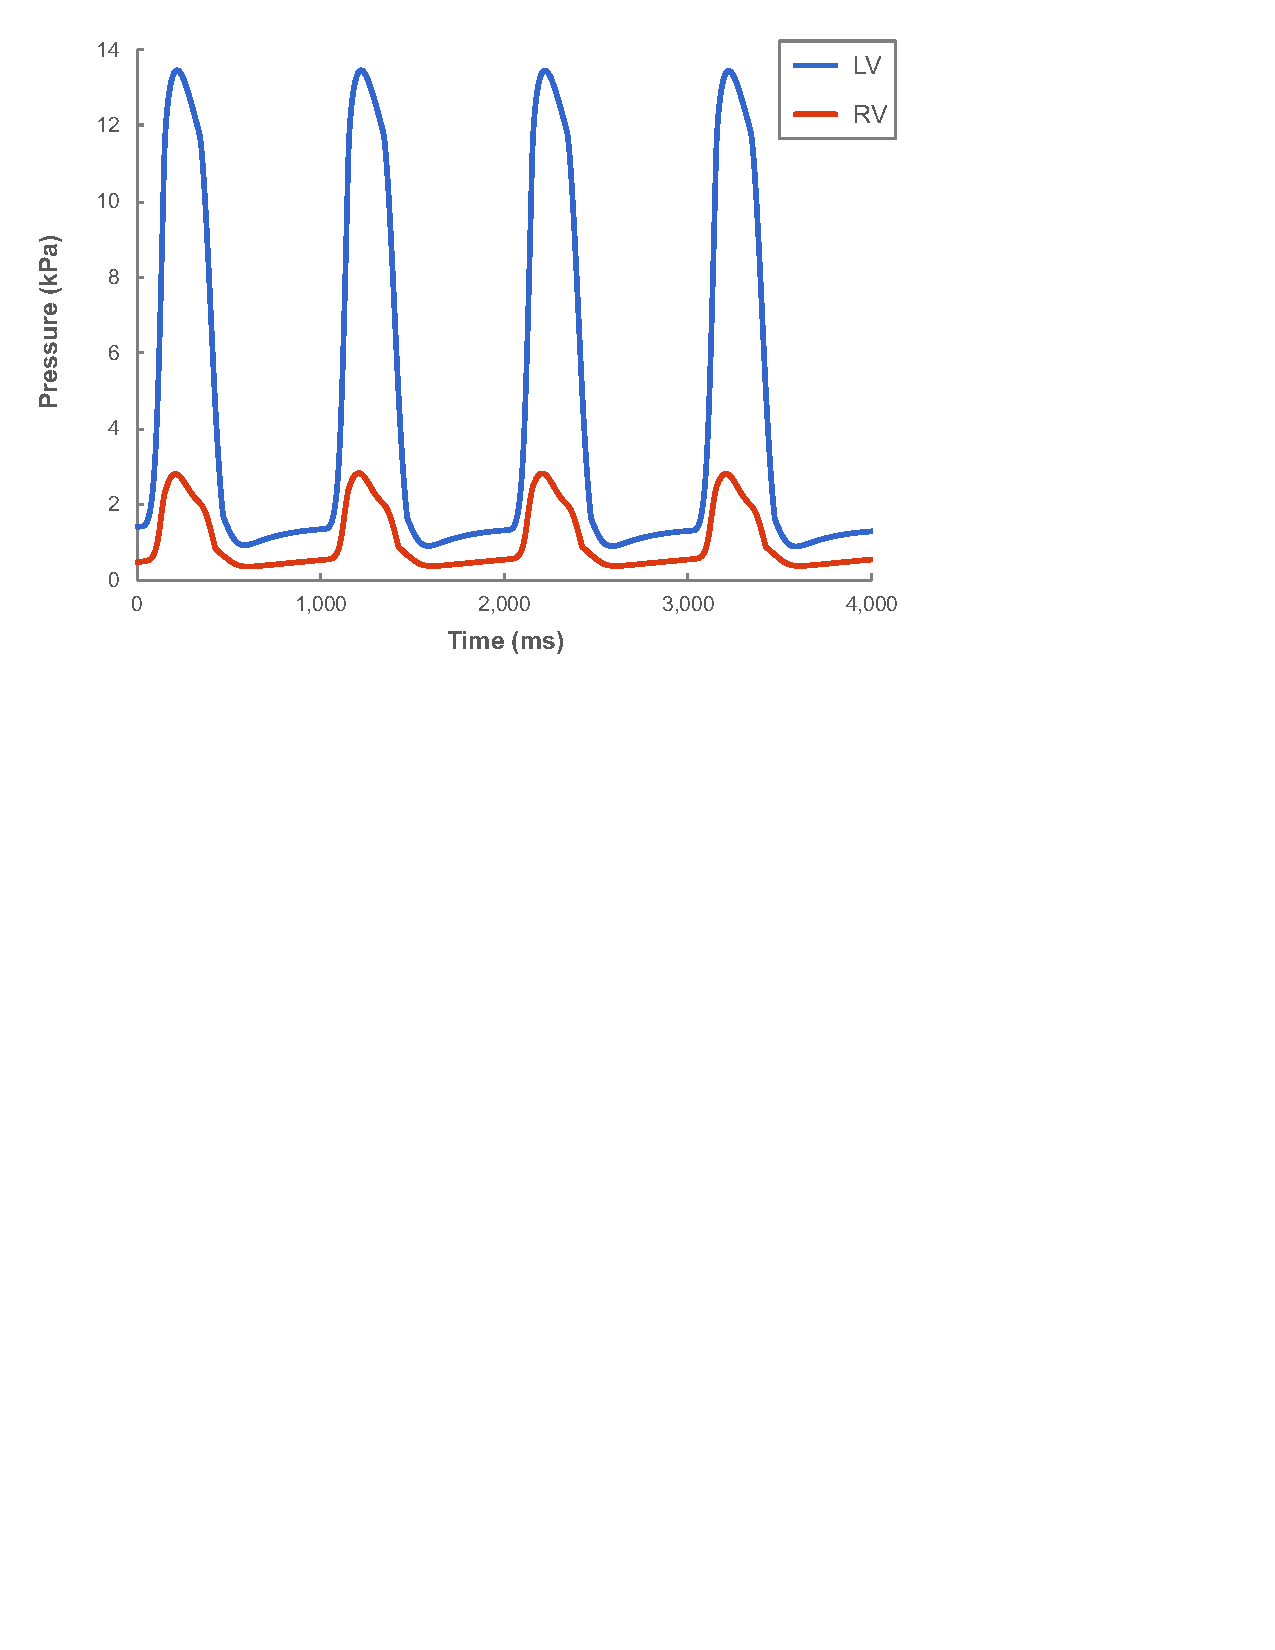
\includegraphics[scale=0.5]{media/4-cardioid/5-pv/pressure_volume-2.pdf}
\label{fig:pv2}}		
%
\caption{Results from Cardioid simulation: (a) P-V loop of left ventricle, (b) pressure time history in left and right ventricles.}
\label{fig:pv}
\end{figure}

\begin{figure}[ht!]
\centering
\subfigure[]{%
		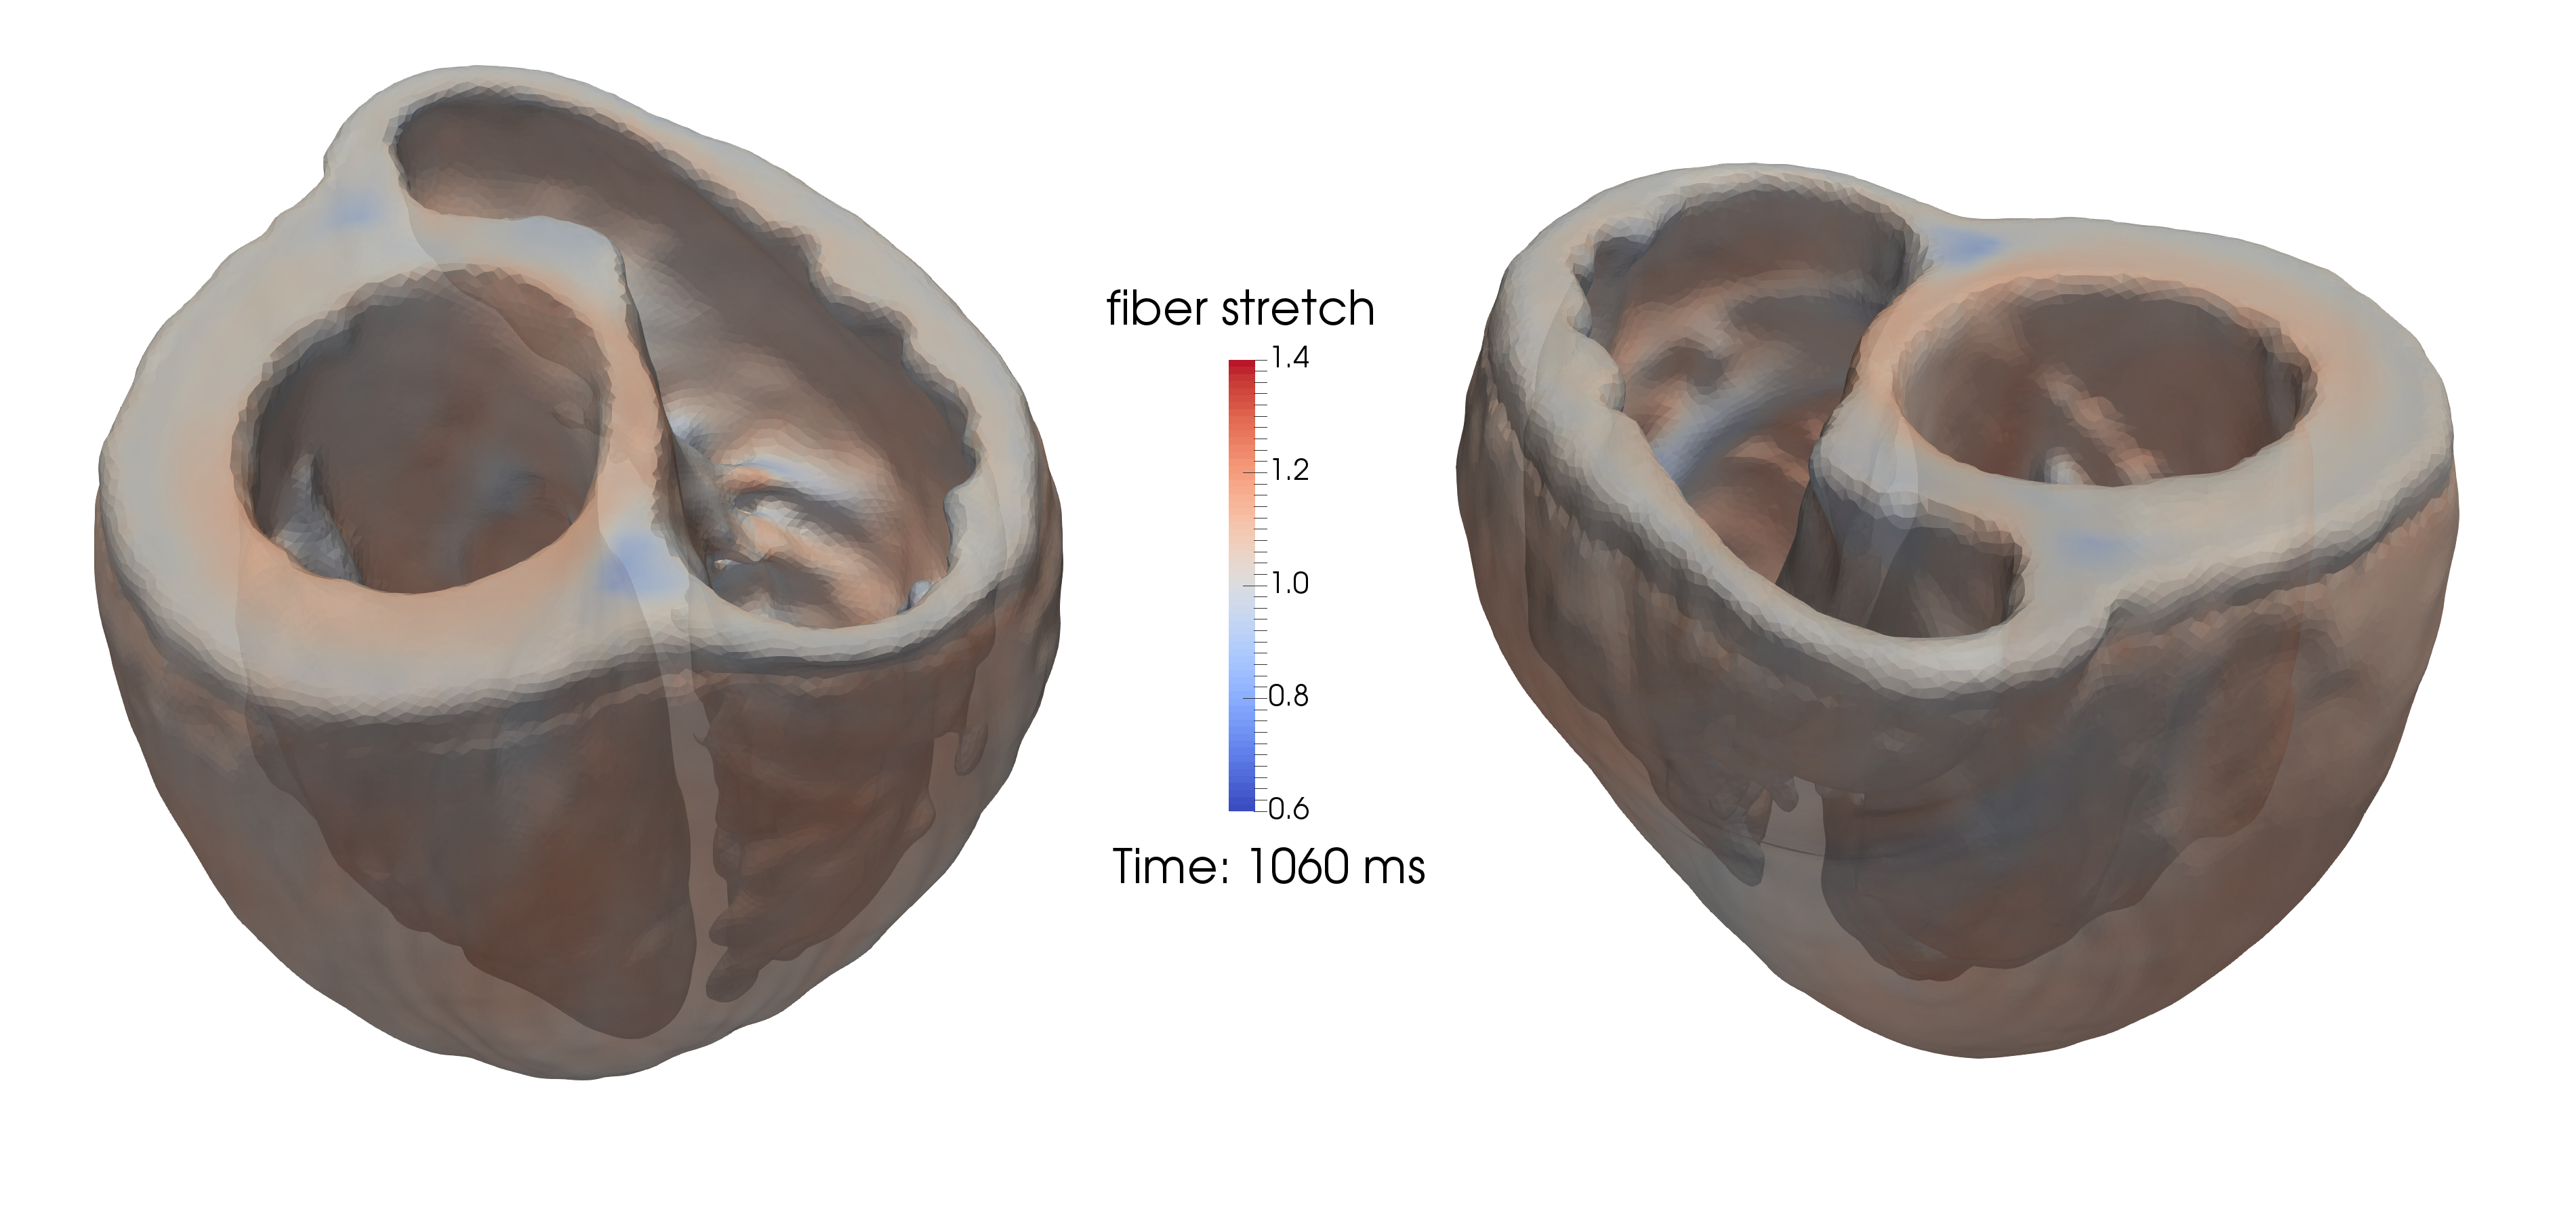
\includegraphics[scale=0.057]{media/4-cardioid/6-vid/a.png}
\label{fig:snaps1}}		
\subfigure[]{%
		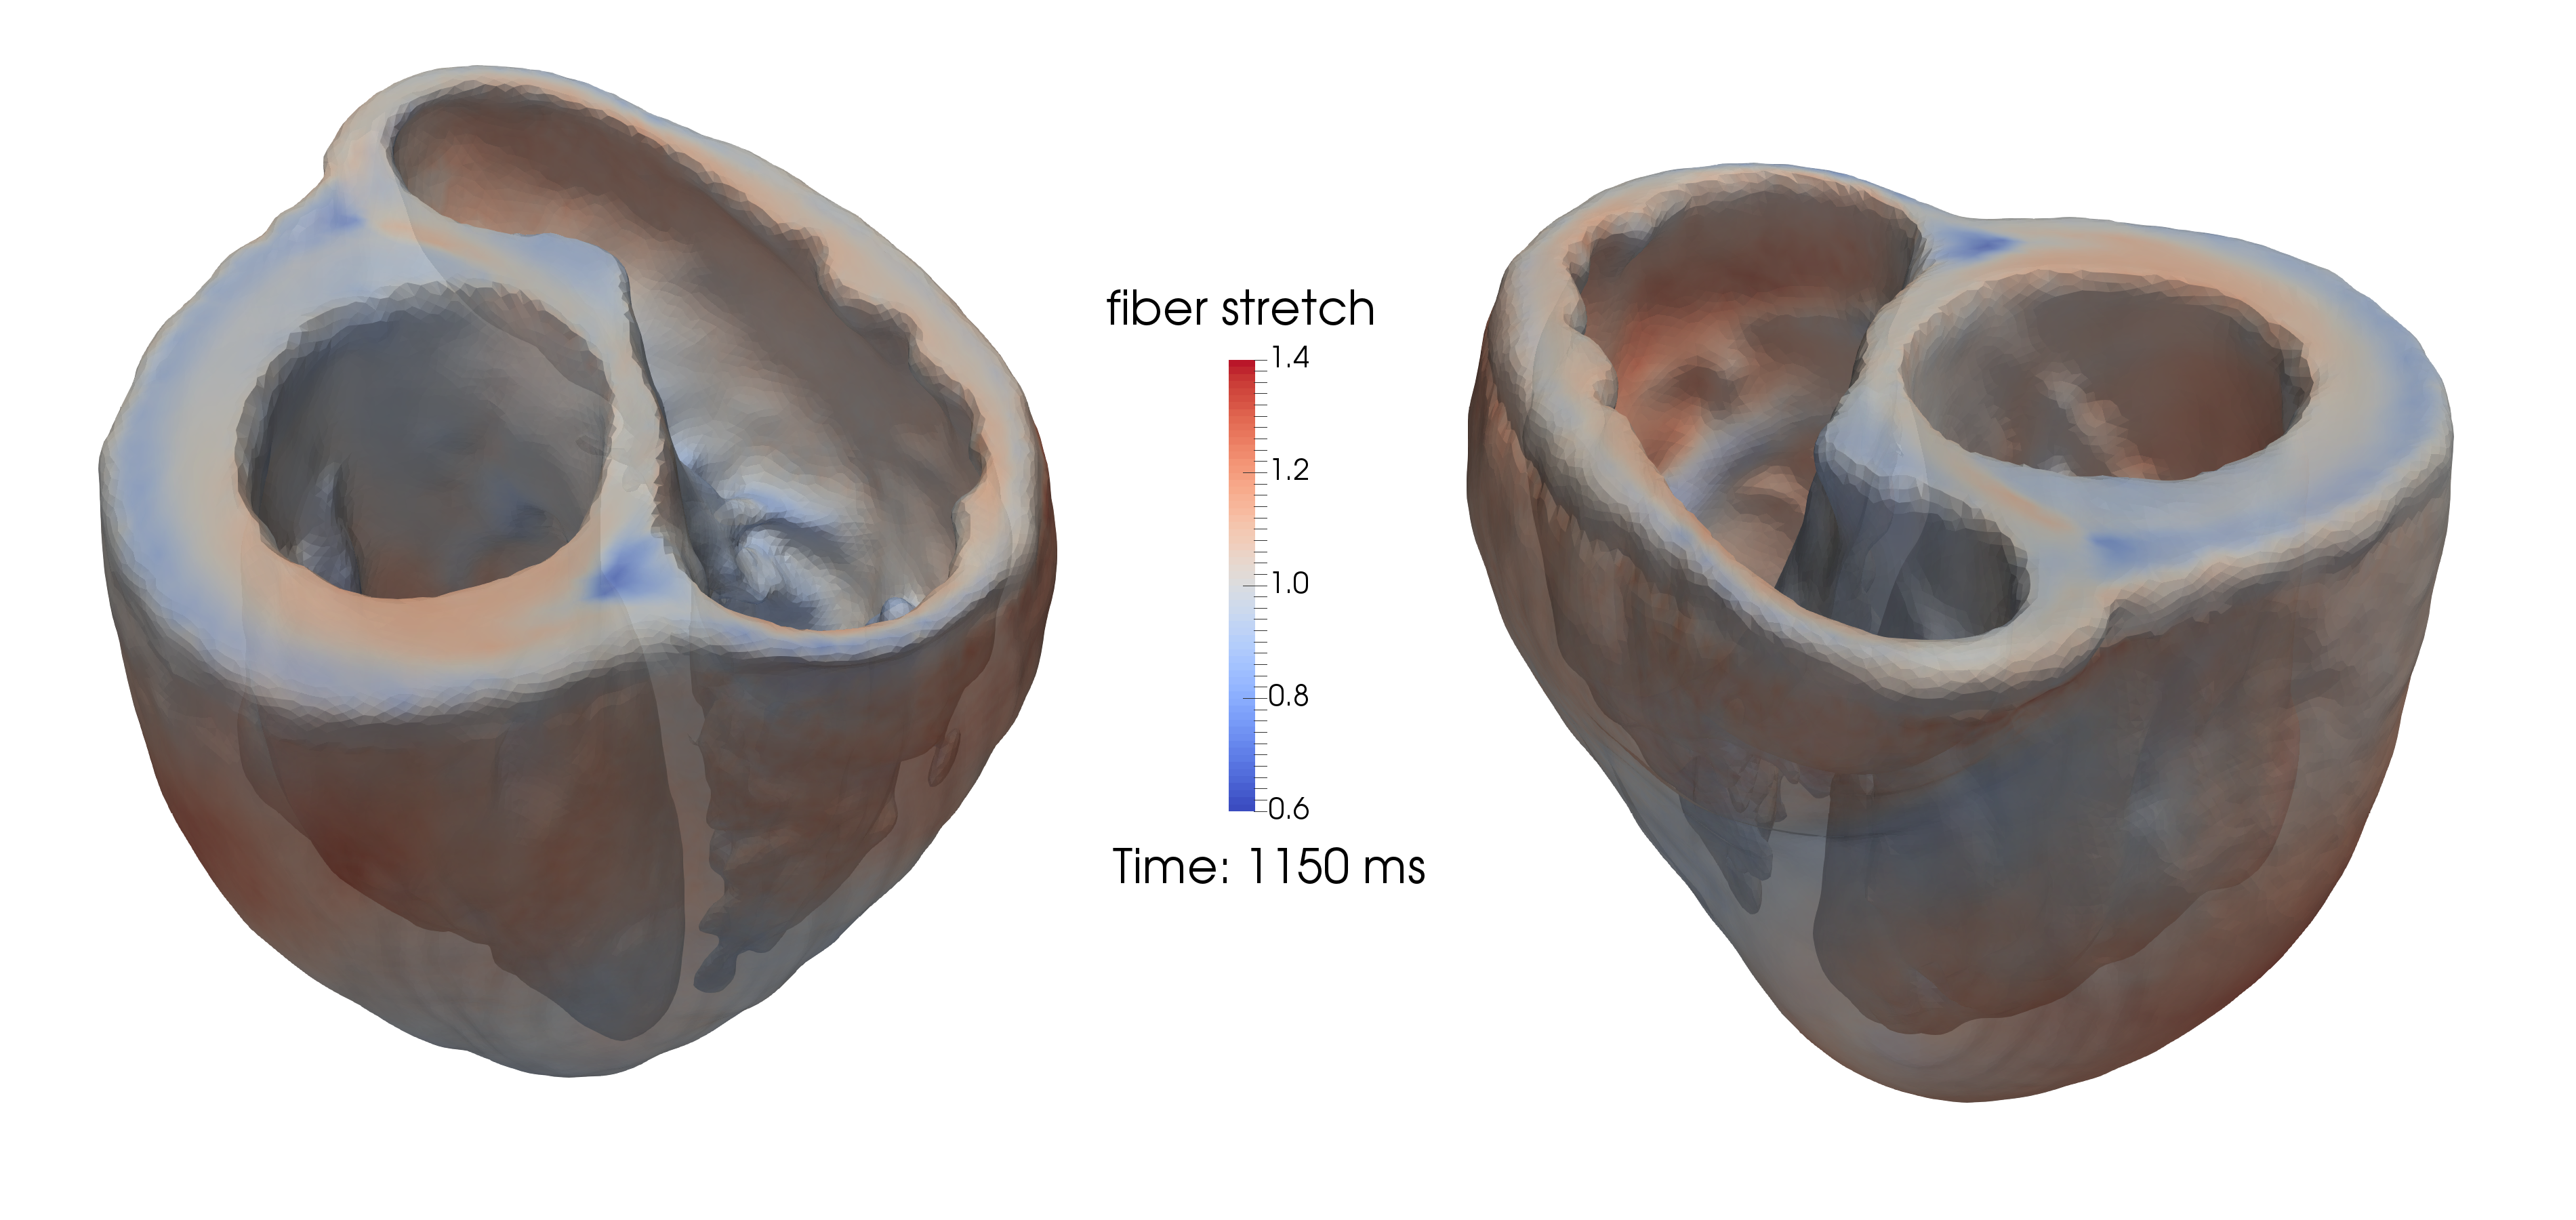
\includegraphics[scale=0.057]{media/4-cardioid/6-vid/b.png}
\label{fig:snaps2}}		
\subfigure[]{%
		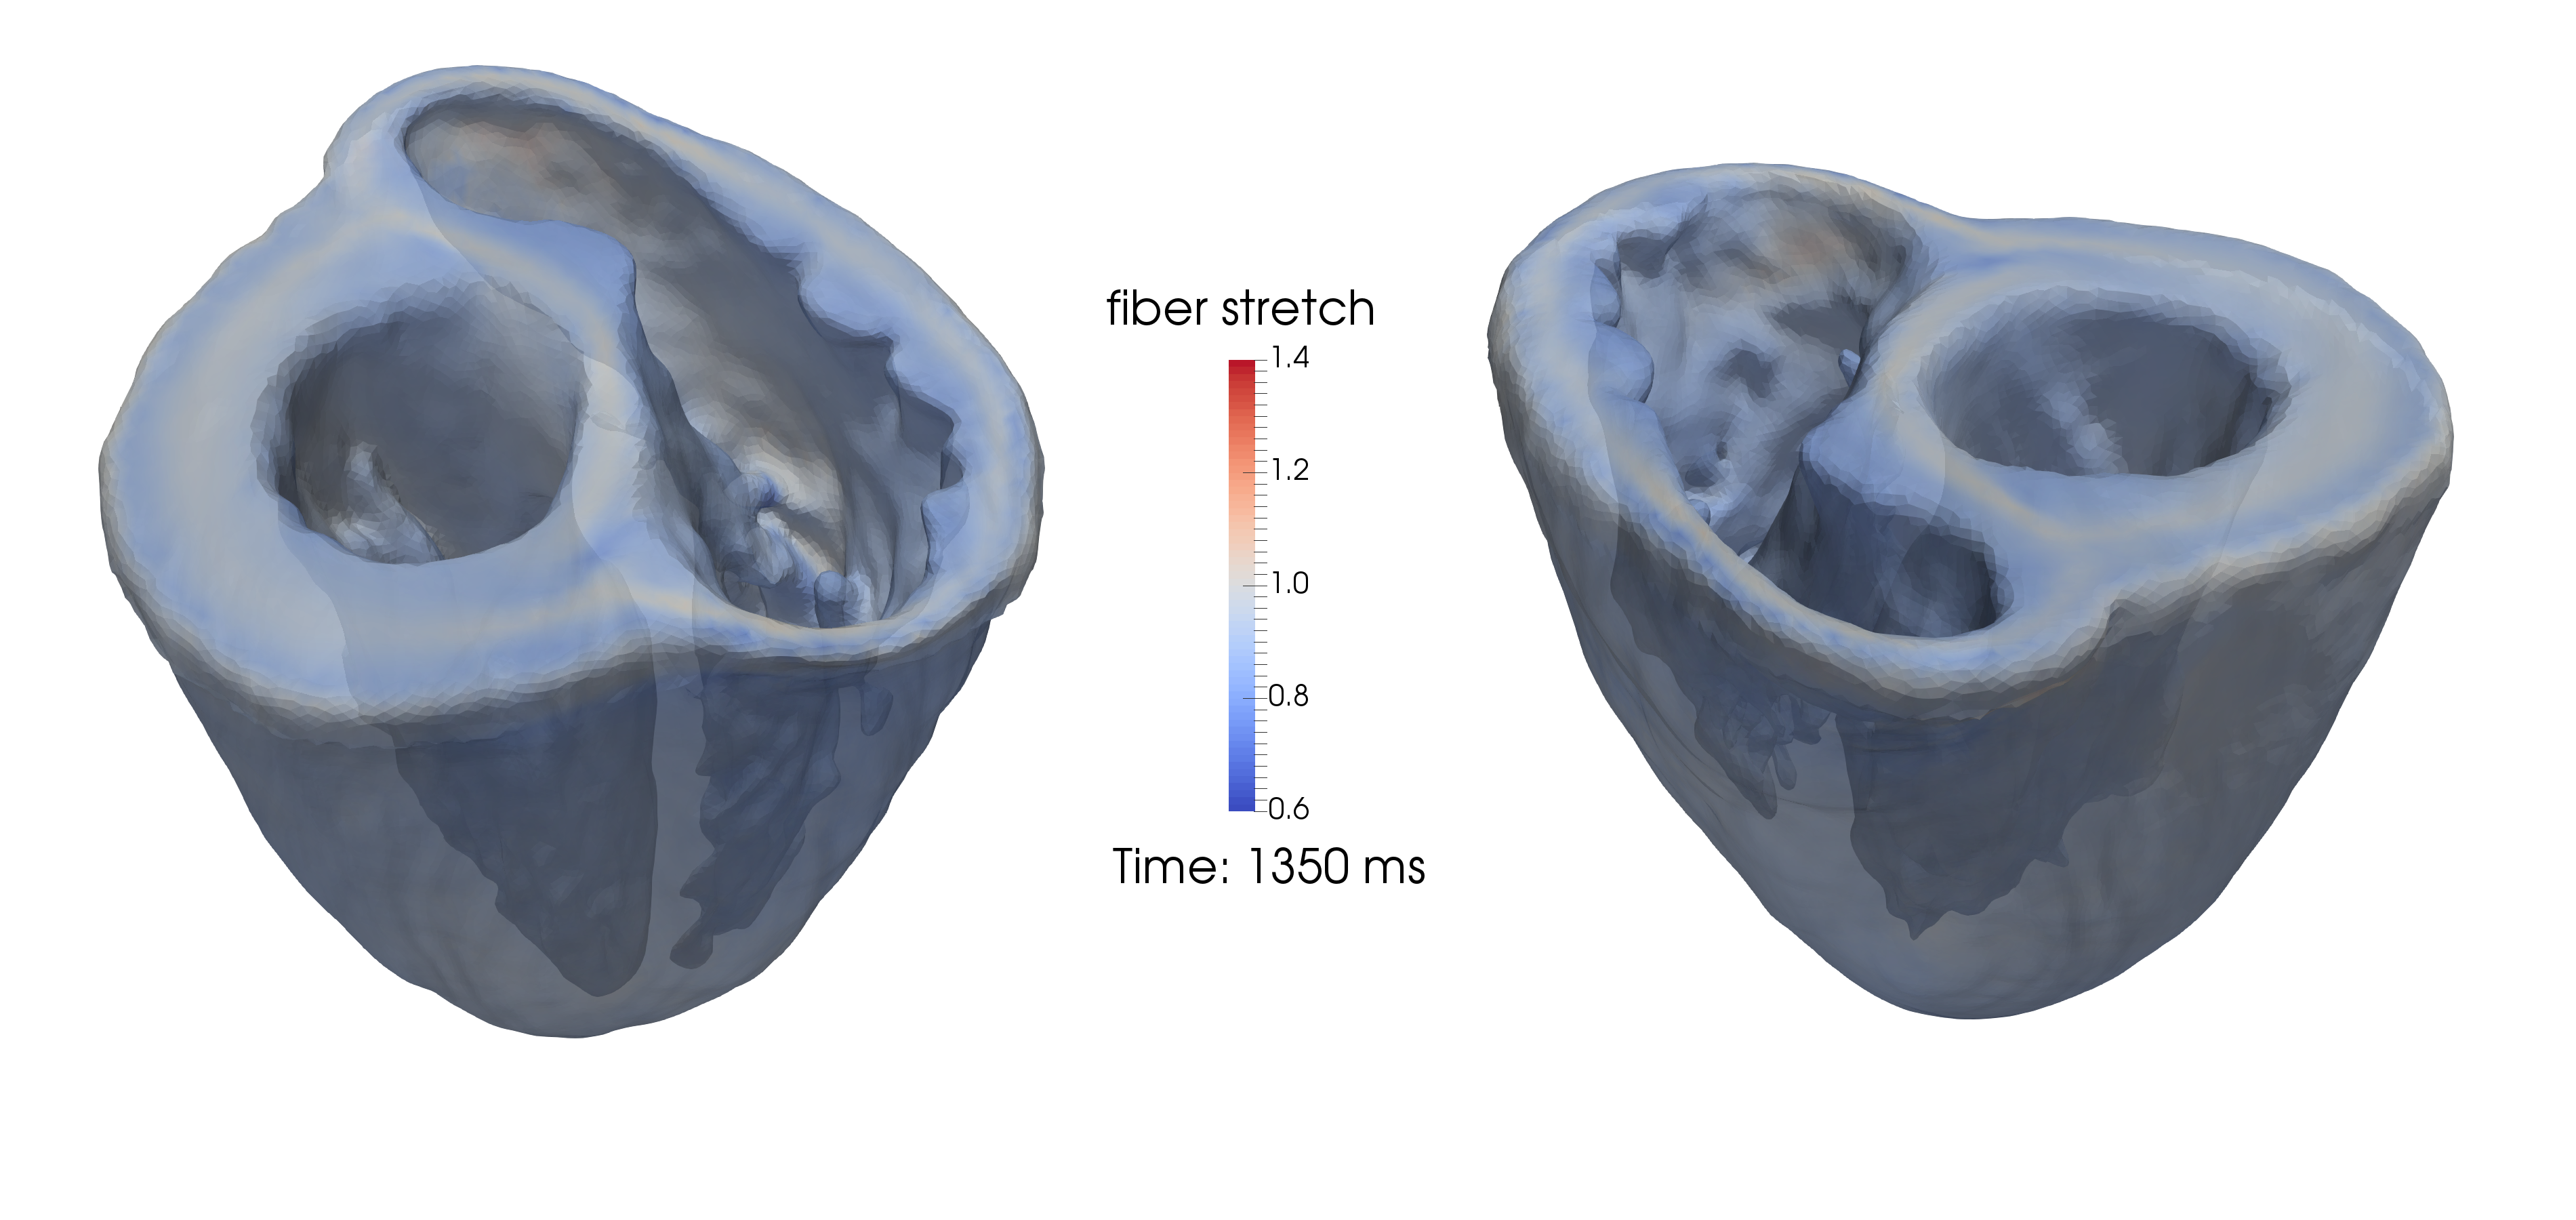
\includegraphics[scale=0.057]{media/4-cardioid/6-vid/c.png}
\label{fig:snapsf3}}		
\subfigure[]{%
		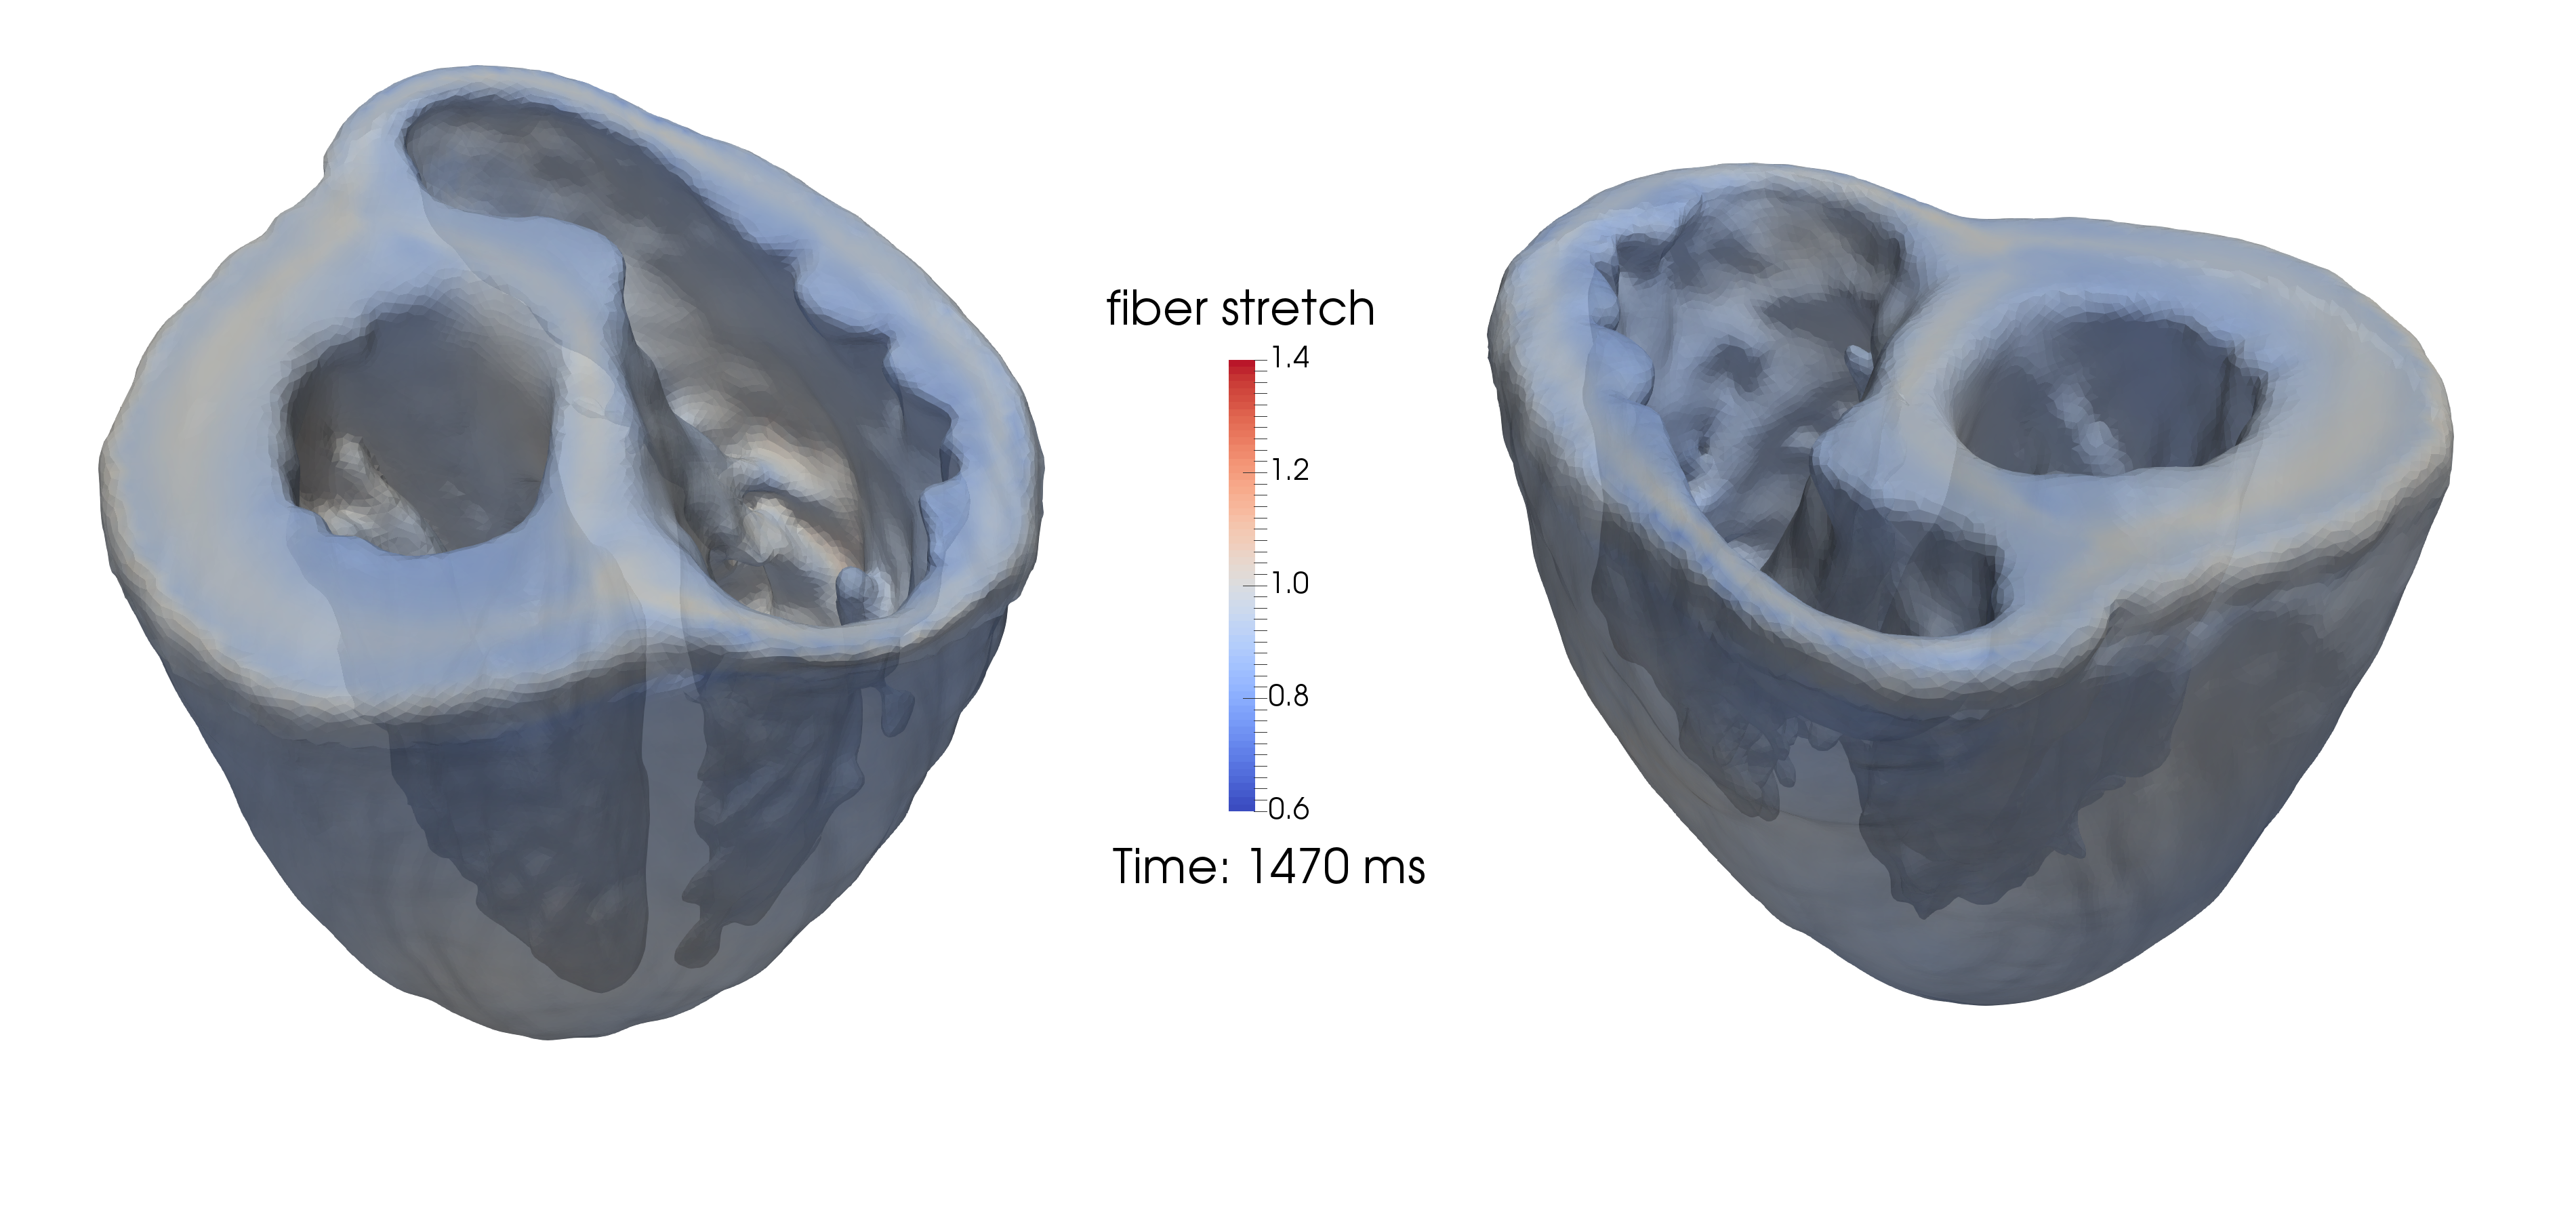
\includegraphics[scale=0.057]{media/4-cardioid/6-vid/d.png}
\label{fig:snaps4}}		
%
\caption{Deformed mesh from Cardioid simulation at different stages of cardiac cycle. Panels (a), (b), (c), and (d) correspond to the stages in the P-V loop denoted in FIGREF ???.}
\label{fig:snaps}
\end{figure}

\begin{figure}[ht]
\centering
\subfigure[]{%
		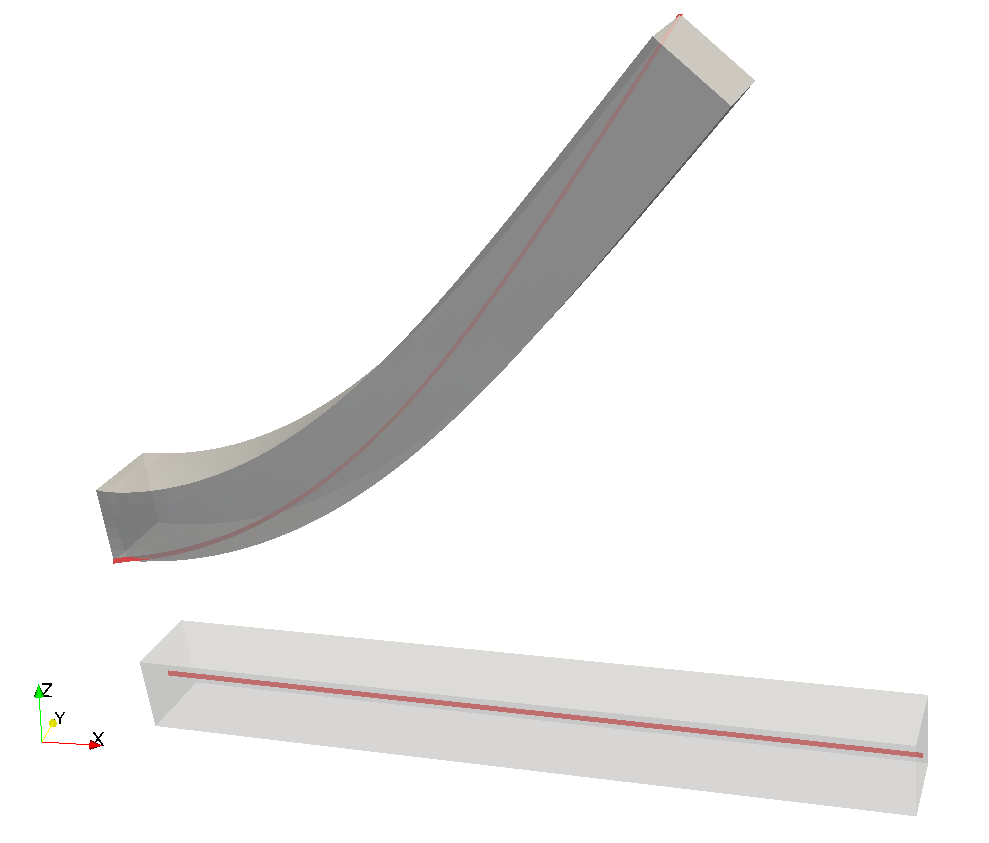
\includegraphics[scale=0.18]{media/5-verif/1-gurev2/gurev2.png}
\label{fig:beams1}}		
\subfigure[]{%
		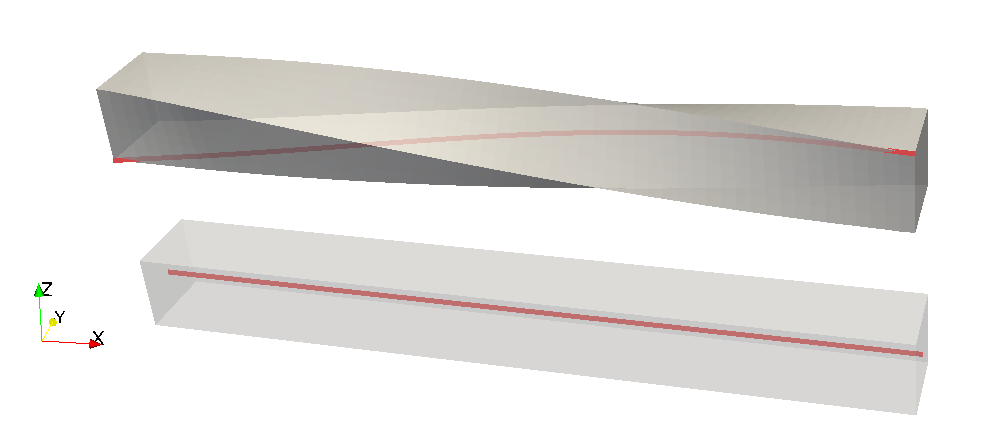
\includegraphics[scale=0.18]{media/5-verif/2-gurev3/gurev3.png}
\label{fig:beams2}}		
\subfigure[]{%
		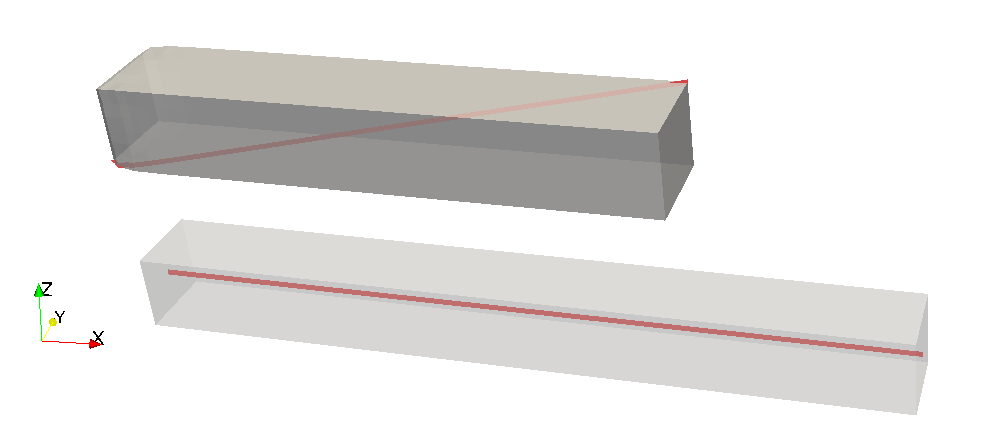
\includegraphics[scale=0.18]{media/5-verif/3-gurev4/gurev4.png}
\label{fig:beams3}}		
\subfigure[]{%
		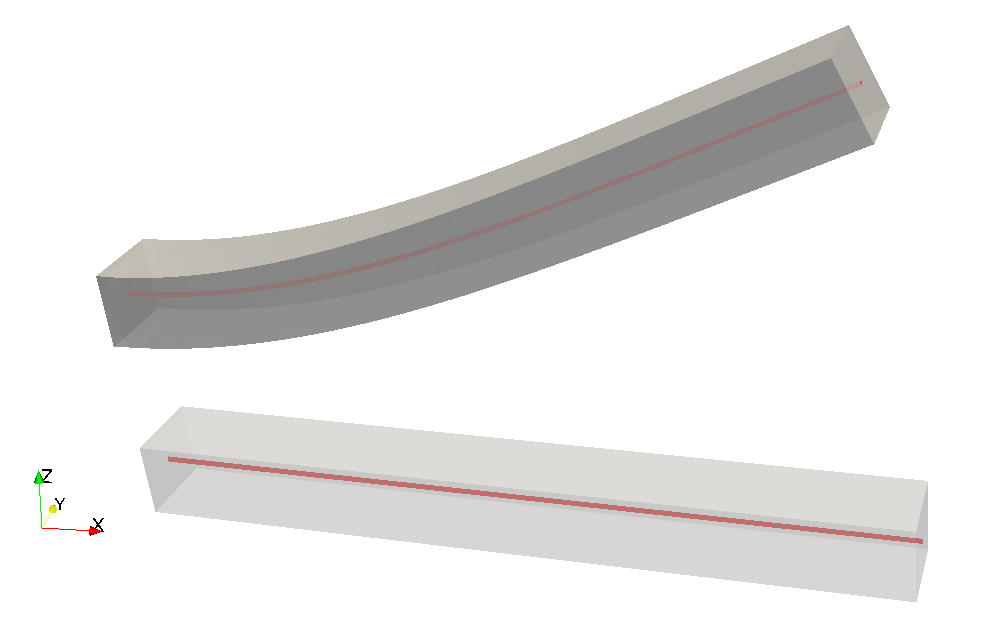
\includegraphics[scale=0.18]{media/5-verif/4-land1/land1.png}
\label{fig:beams4}}		
%
\caption{Undeformed (bottom) and deformed (top) configurations for cantilever beam verification problems: (a) Gurev P2: bending, (b) Gurev P3: torsion, c) Gurev P4: active contraction, and (d) Land P1: bending. The red curve denotes the curve over which displacements and positions are recorded for comparison of results.}
\label{fig:beams}
\end{figure}

\begin{figure}[ht]
\centering
\subfigure[]{%
		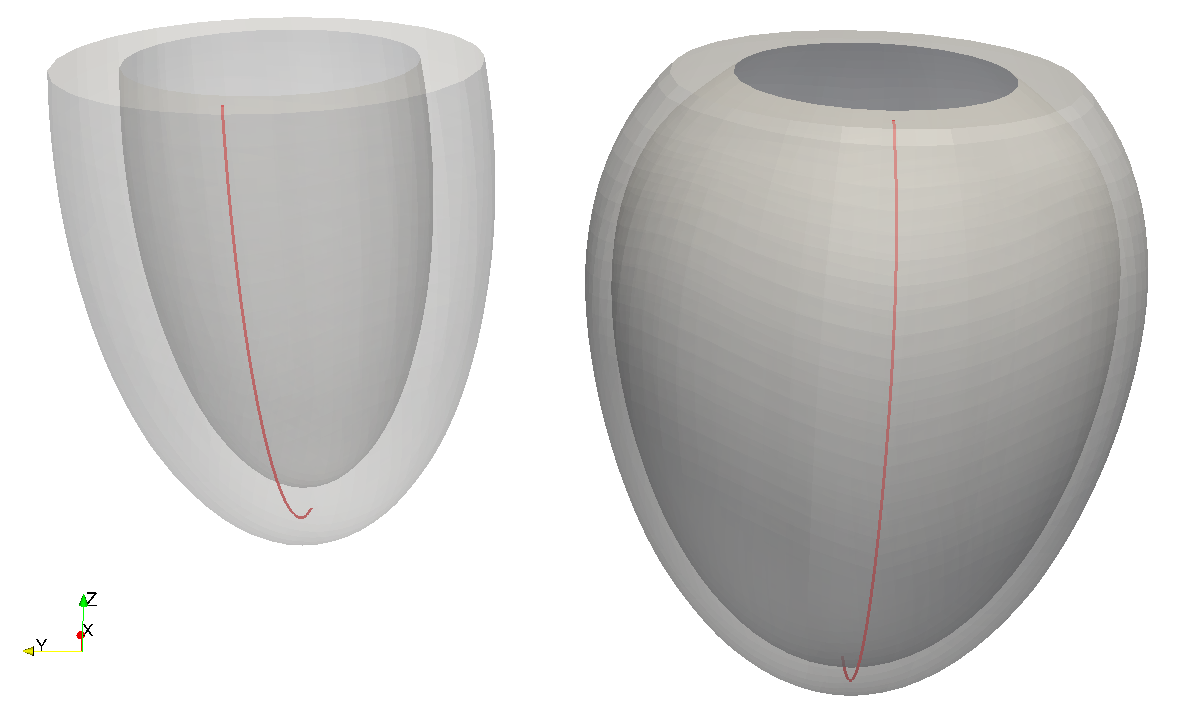
\includegraphics[scale=0.18]{media/5-verif/5-land2/land2-1.png}
\label{fig:ventricles1}}		
\subfigure[]{%
		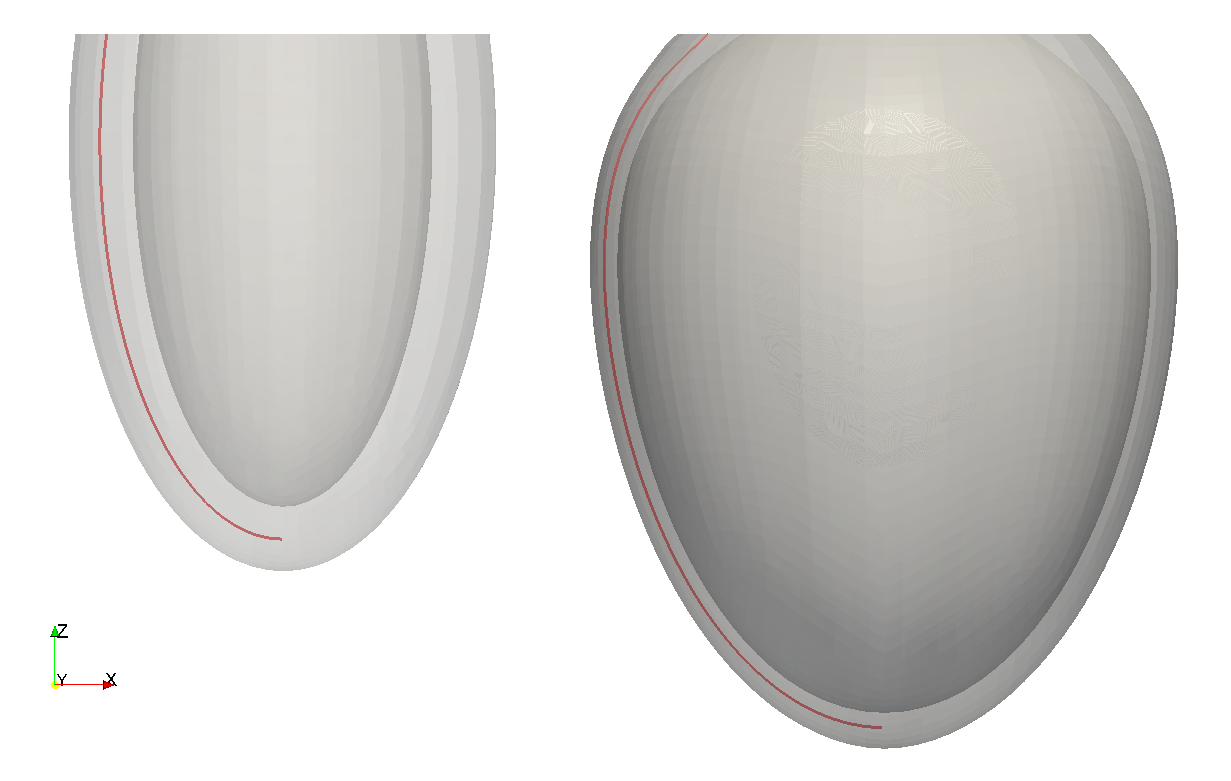
\includegraphics[scale=0.18]{media/5-verif/5-land2/land2-2.png}
\label{fig:ventricles2}}		
\subfigure[]{%
		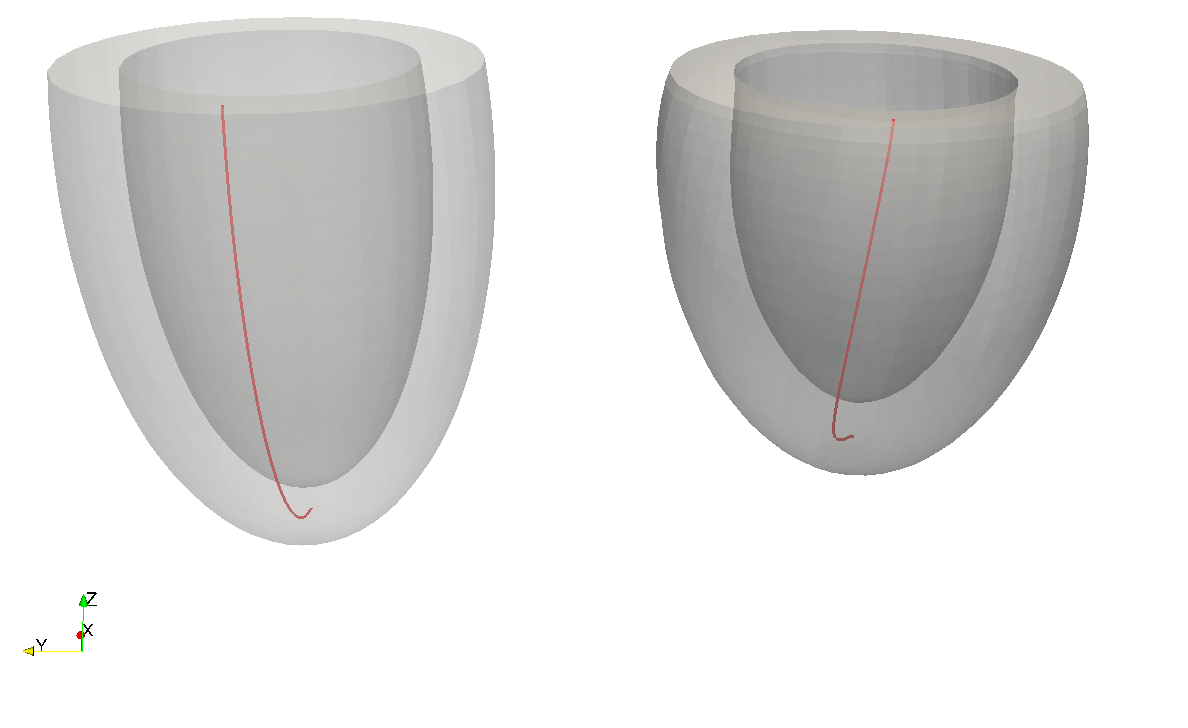
\includegraphics[scale=0.18]{media/5-verif/6-land3/land3-1.png}
\label{fig:ventricles3}}		
\subfigure[]{%
		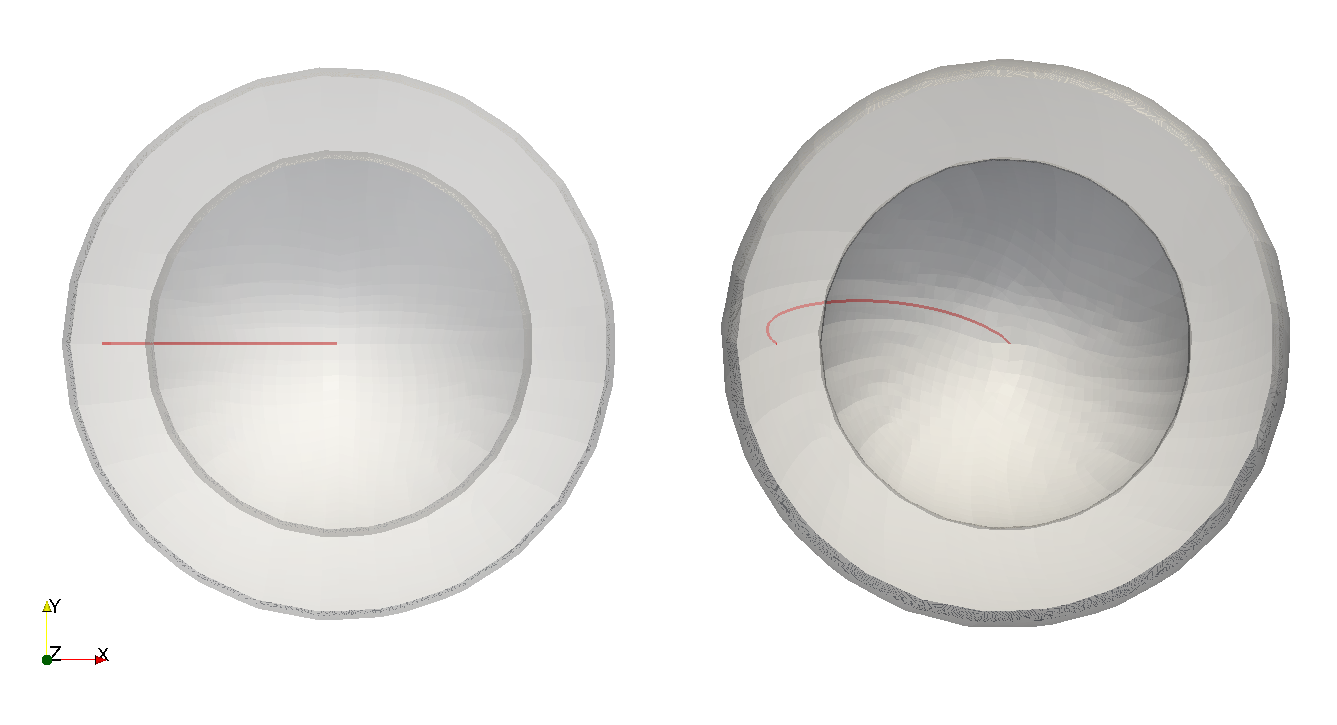
\includegraphics[scale=0.16]{media/5-verif/6-land3/land3-2.png}
\label{fig:ventricles4}}		
%
\caption{Undeformed (left) and deformed (right) configurations for single ventricle verification problems: (a,b) Land P2: inflation, and (c,d) Land P3: inflation and active contraction. The red curve denotes the curve over which displacements and positions are recorded for comparison of results.}
\label{fig:ventricles}
\end{figure}

\begin{figure}[ht]
\centering
\subfigure[]{%
		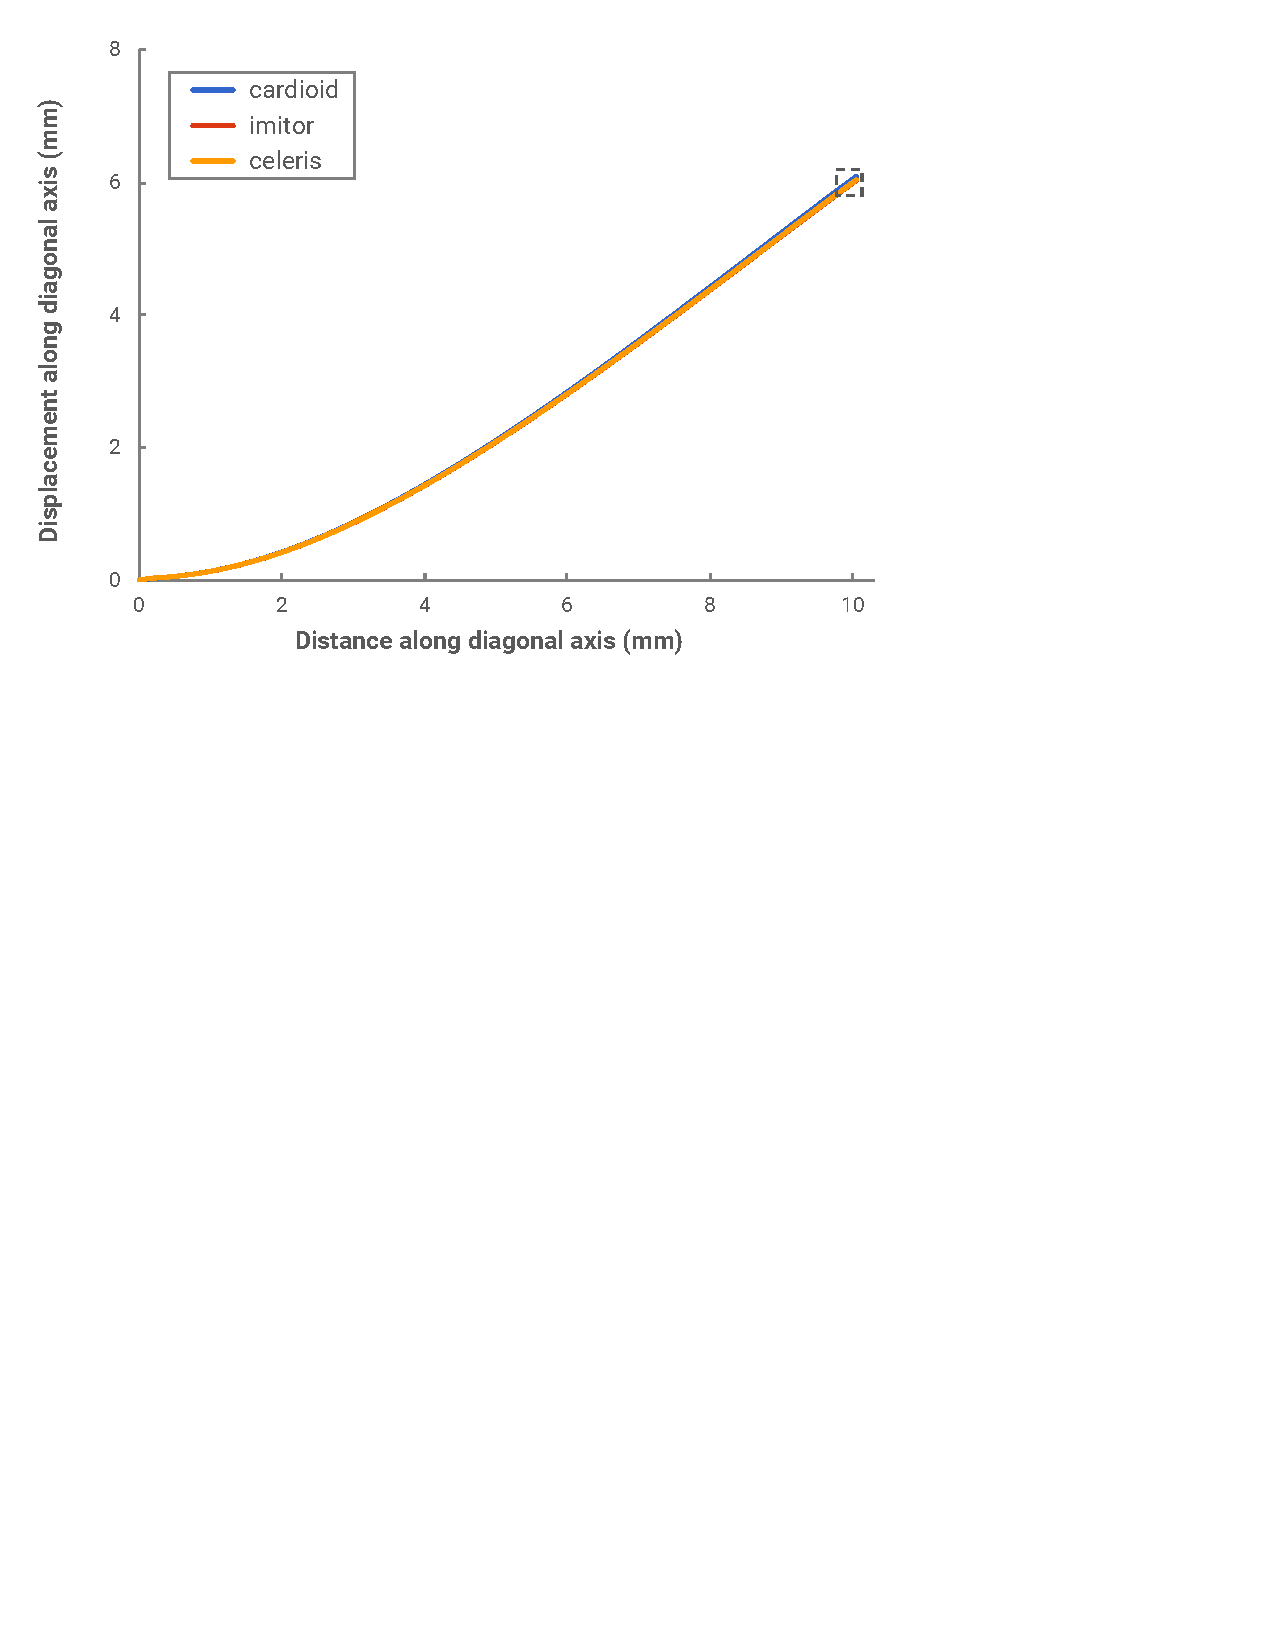
\includegraphics[scale=0.48]{media/5-verif/1-gurev2/gurev2-1.pdf}
\label{fig:gurev2-1}}		
\subfigure[]{%
		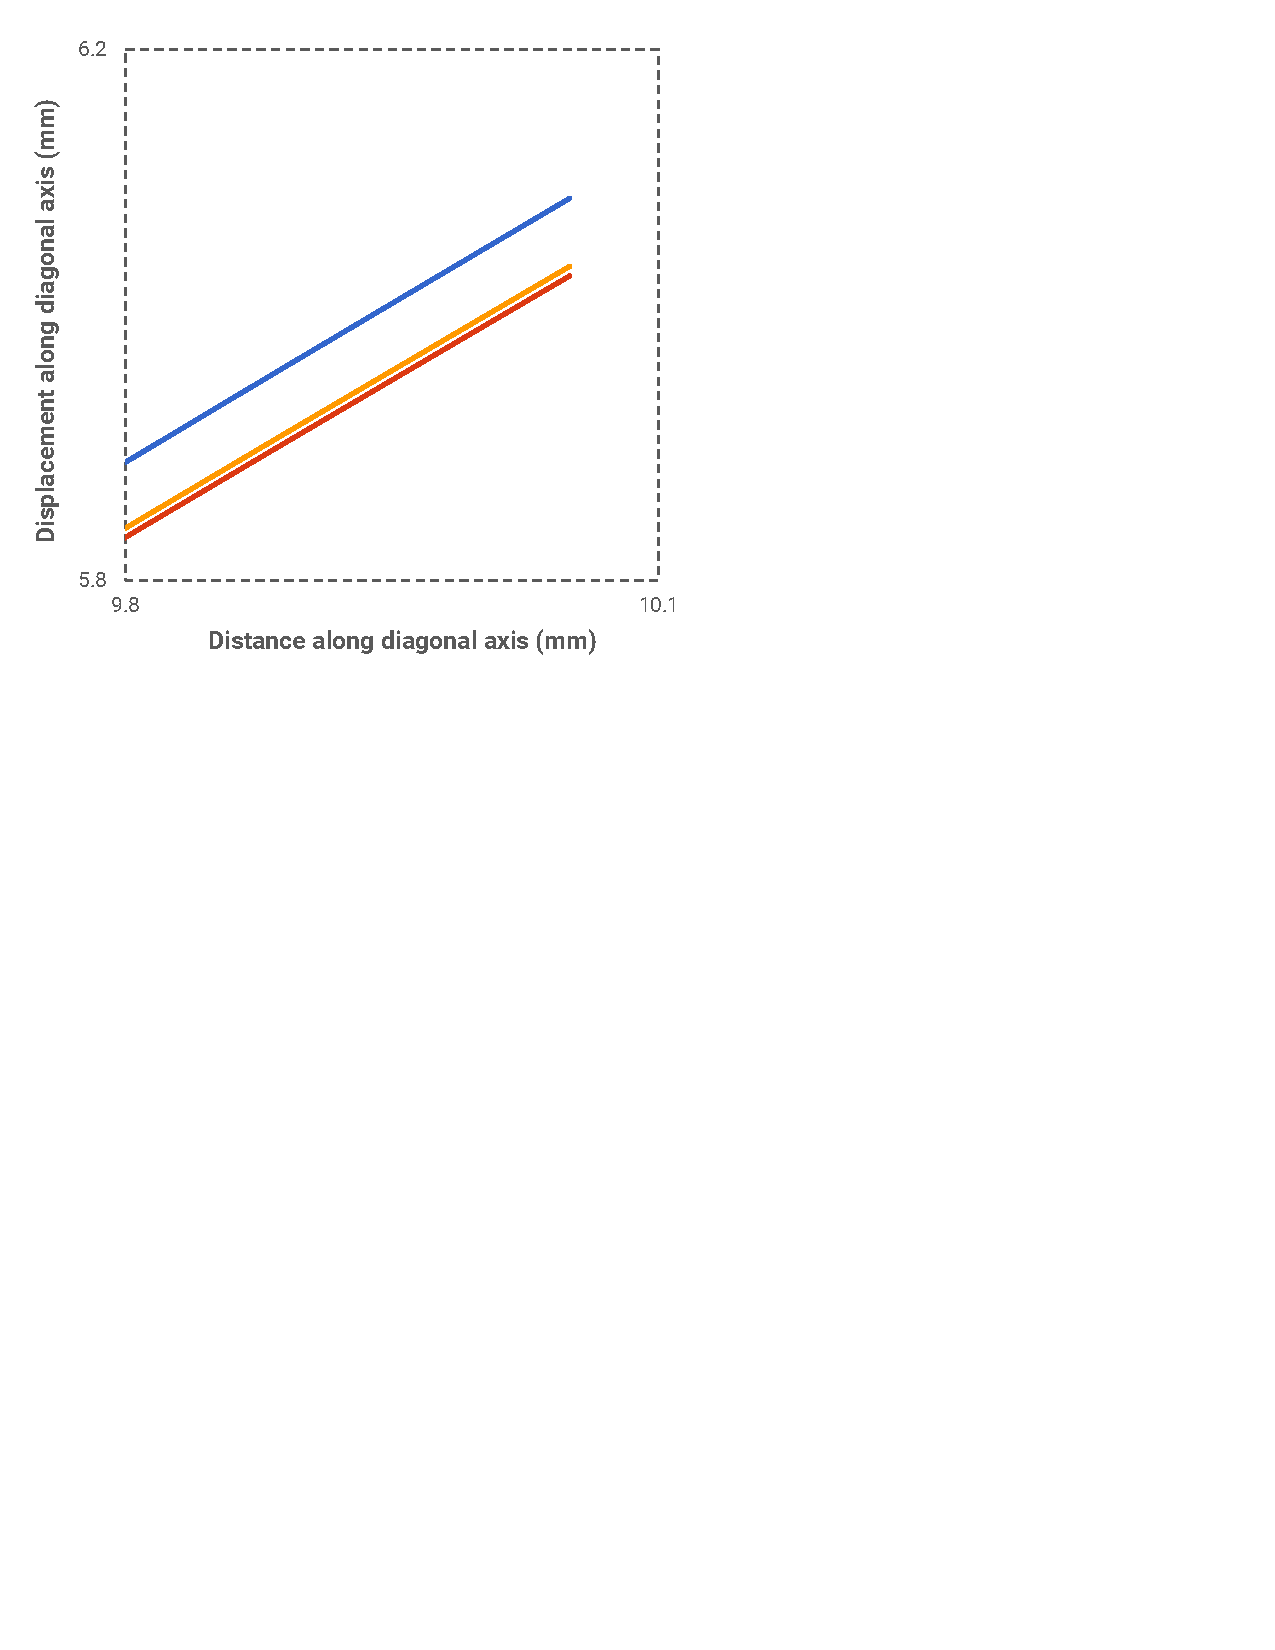
\includegraphics[scale=0.48]{media/5-verif/1-gurev2/gurev2-2.pdf}
\label{fig:gurev2-2}}		
%
\caption{Results for Gurev P2 verification problem: (a) Displacement magnitude along diagonal axis, with (b) details for the free end of the beam}
\label{fig:gurev2}
\end{figure}

\begin{figure}[ht!]
\centering
\subfigure[]{%
		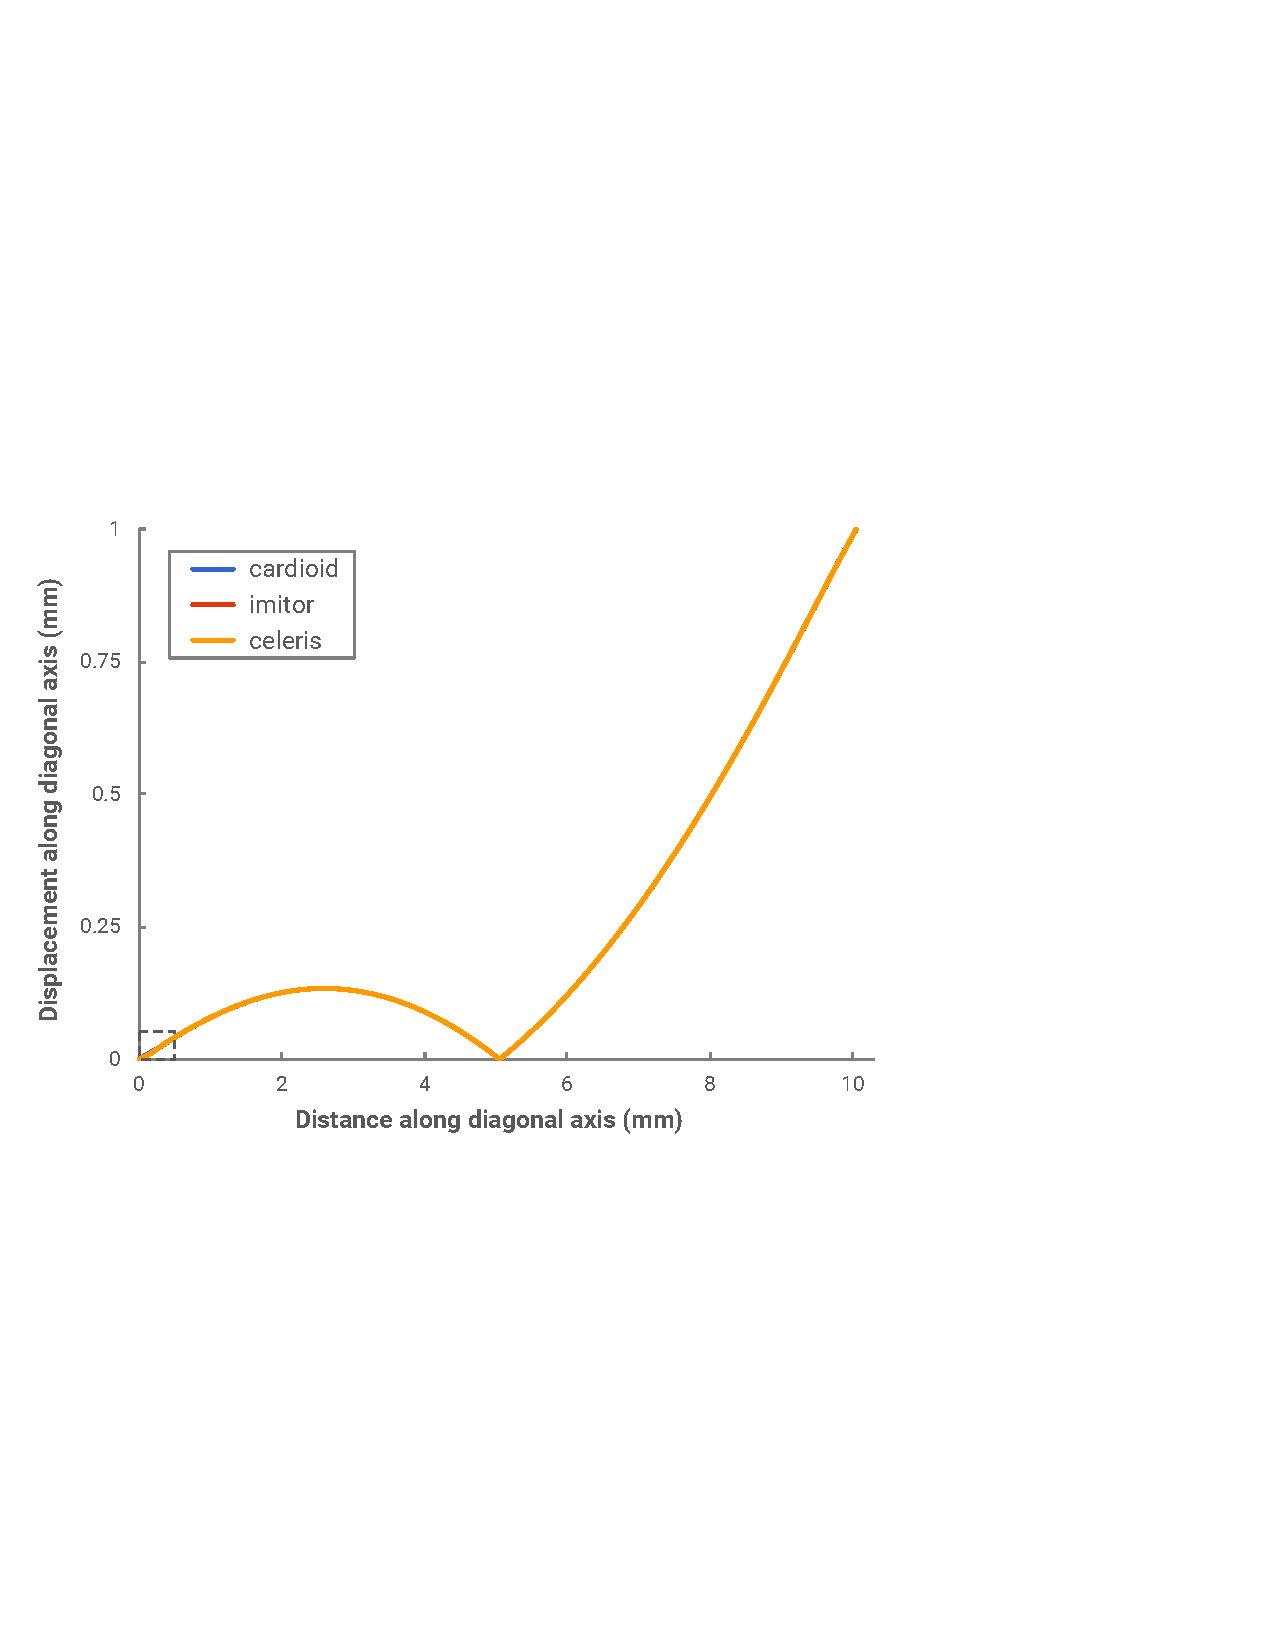
\includegraphics[scale=0.48]{media/5-verif/2-gurev3/gurev3-1.pdf}
\label{fig:gurev3-1}}		
\subfigure[]{%
		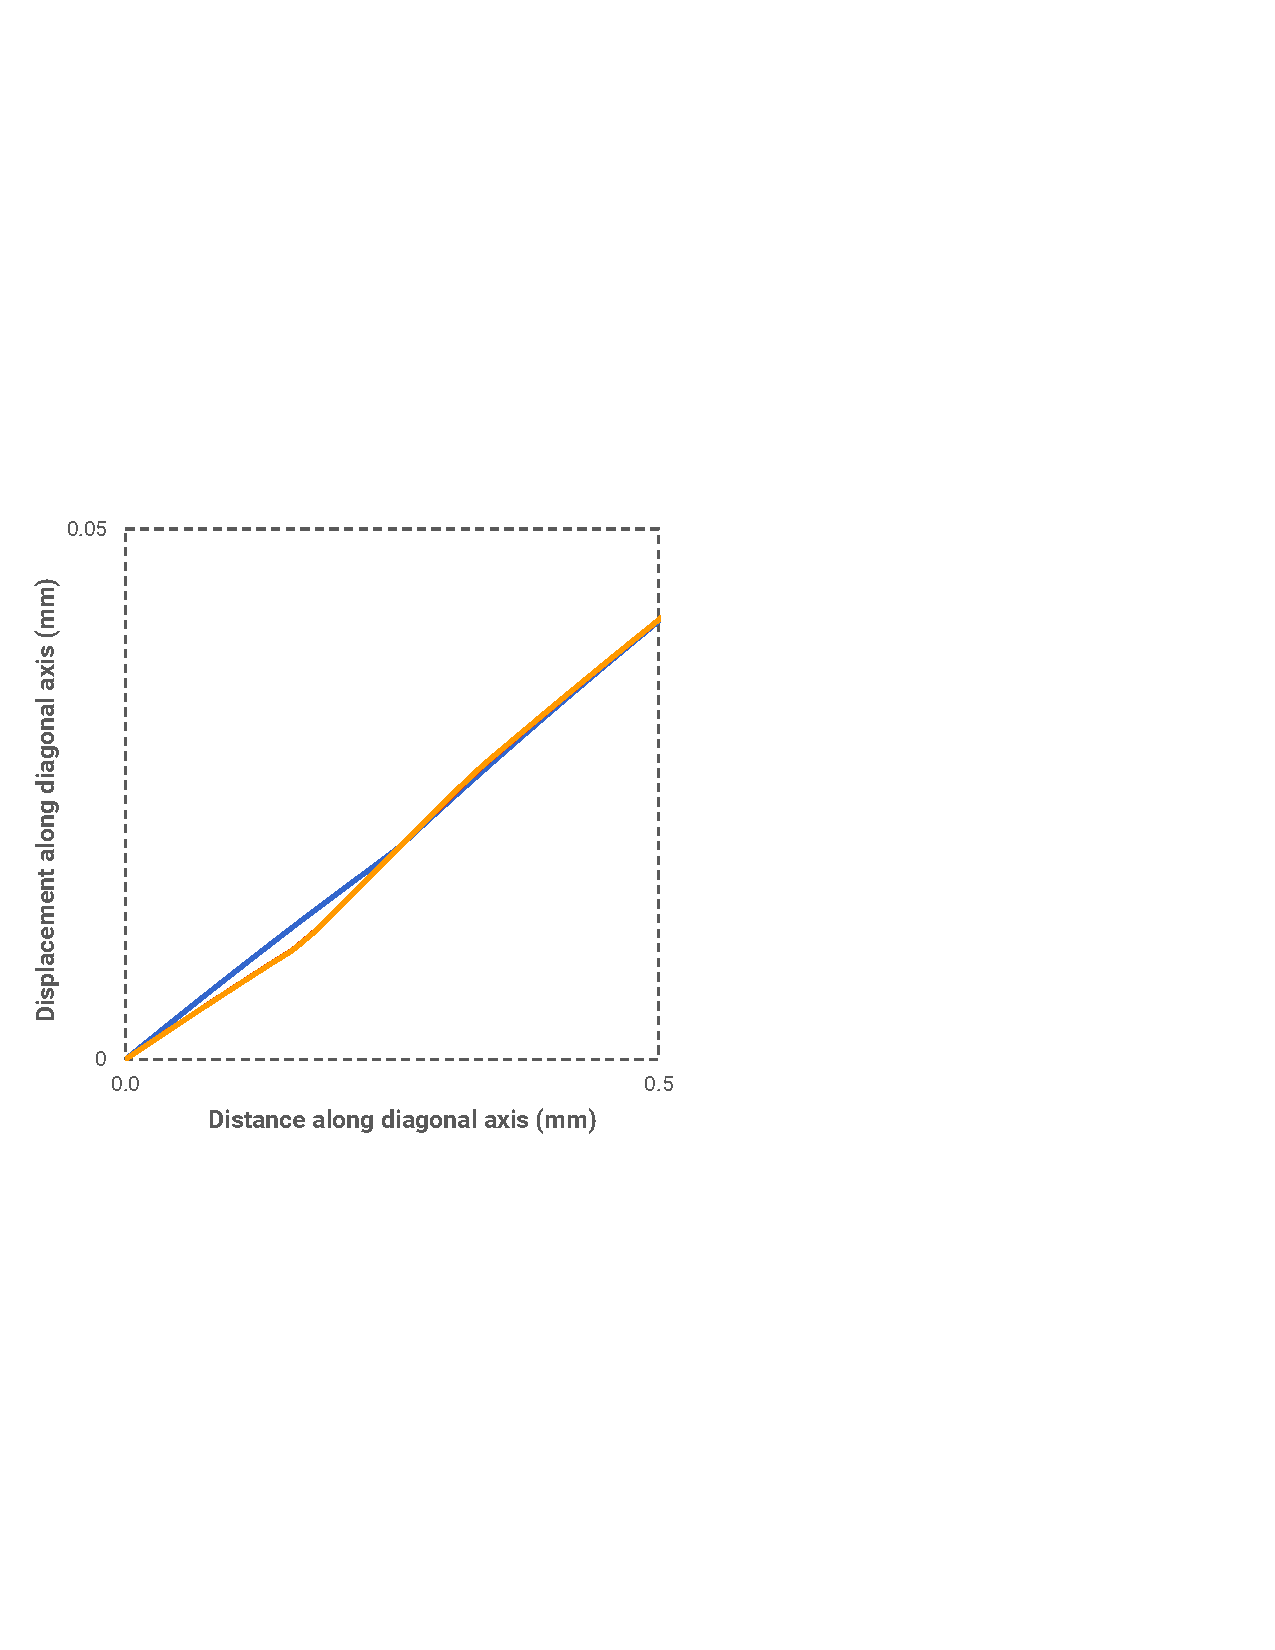
\includegraphics[scale=0.48]{media/5-verif/2-gurev3/gurev3-2.pdf}
\label{fig:gure3-2}}		
%
\caption{Results for Gurev P3 verification problem: (a) Displacement magnitude along diagonal axis, with (b) details for the fixed end of the beam. The results for imitor and Celeris are indistinguishable in these plots.}
\label{fig:gurev3}
\end{figure}

\begin{figure}[ht!]
\centering
\subfigure[]{%
		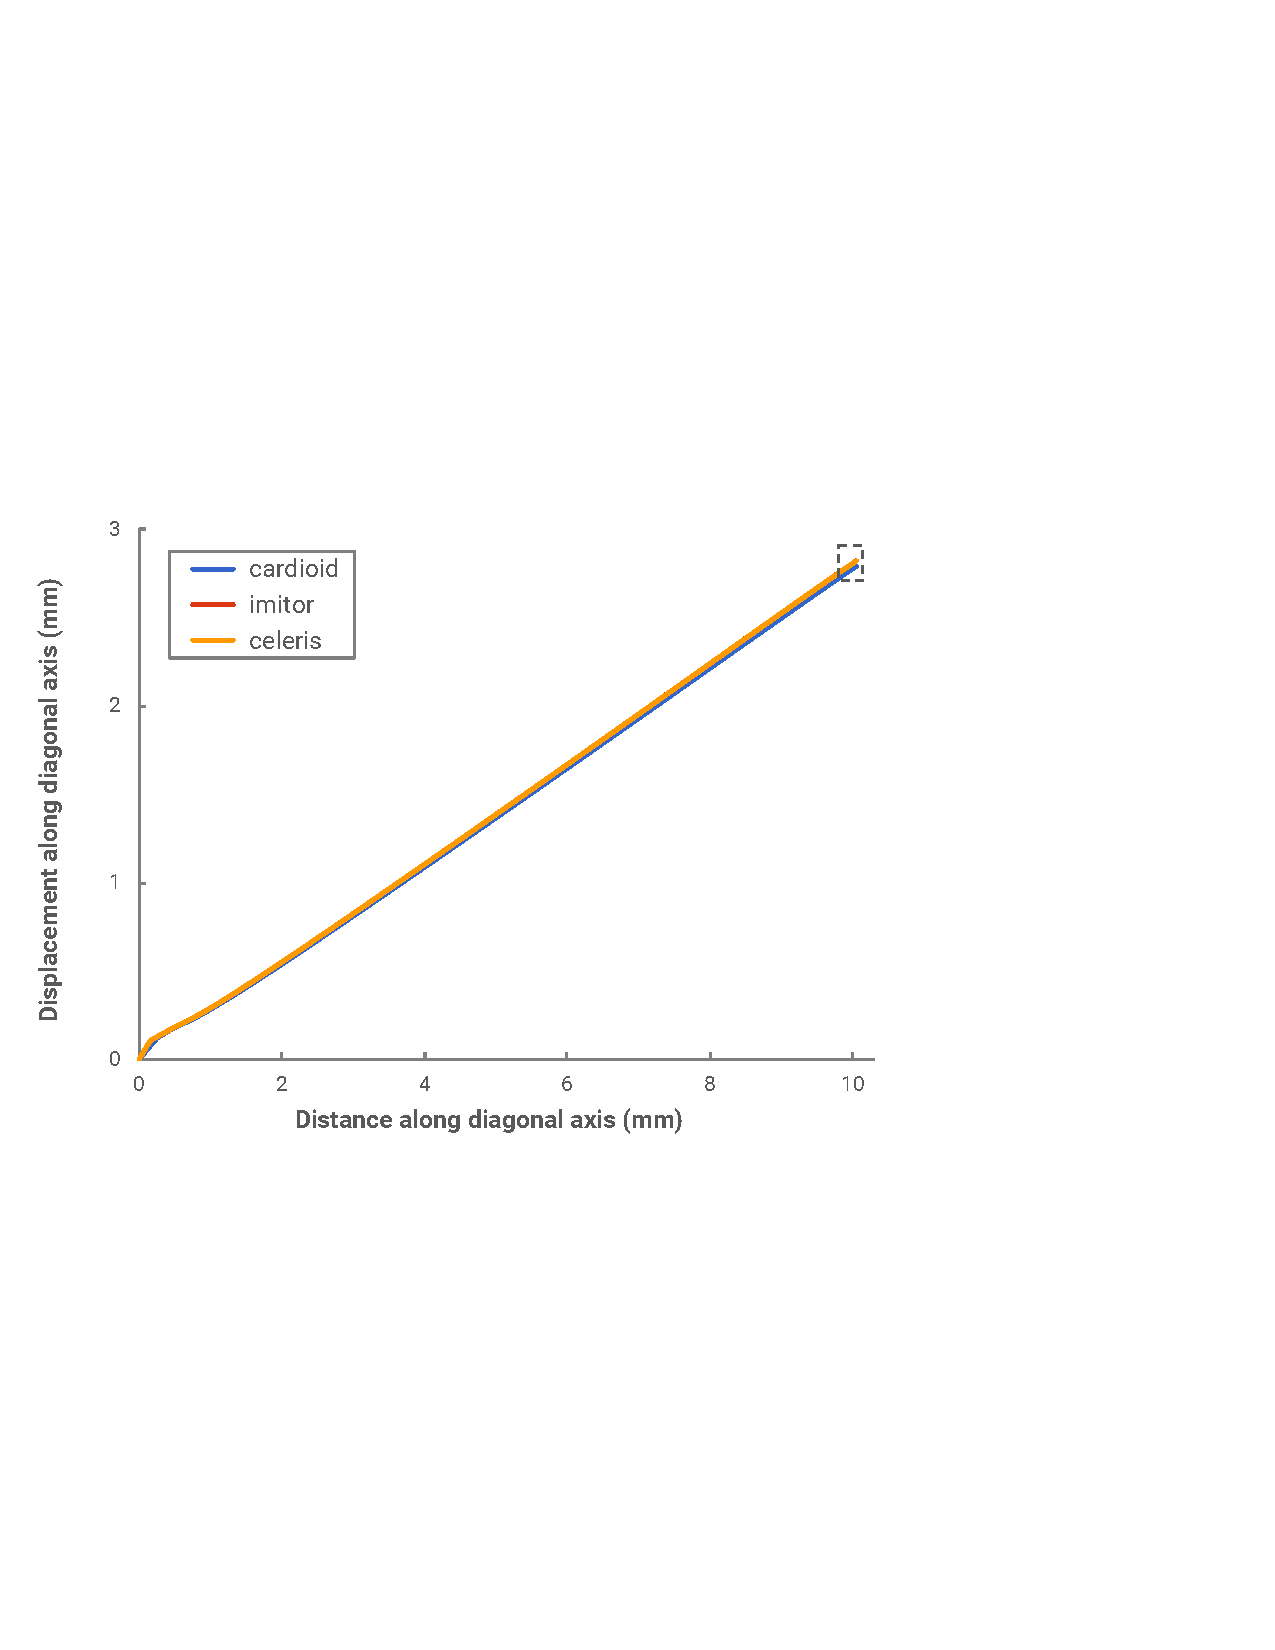
\includegraphics[scale=0.48]{media/5-verif/3-gurev4/gurev4-1.pdf}
\label{fig:gurev4-1}}		
\subfigure[]{%
		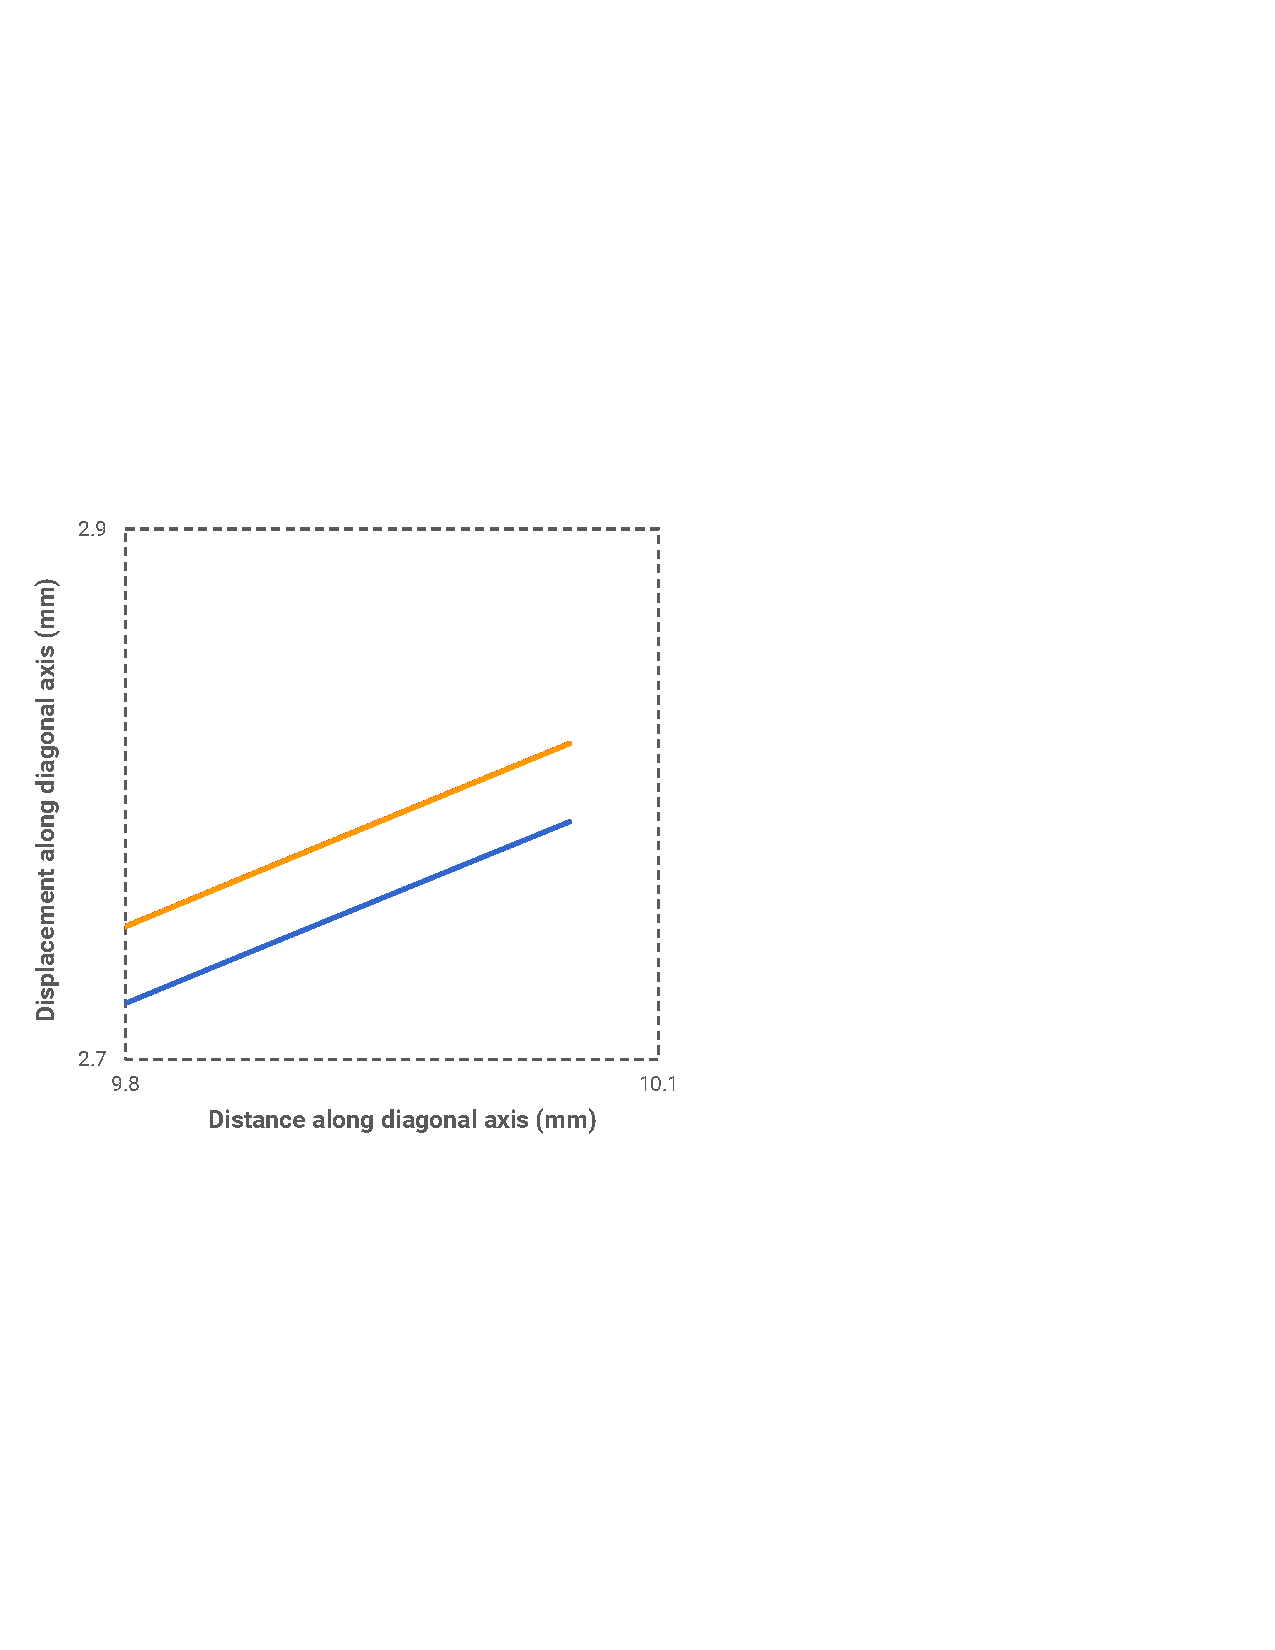
\includegraphics[scale=0.48]{media/5-verif/3-gurev4/gurev4-2.pdf}
\label{fig:gurev4-2}}		
%
\caption{Results for Gurev P4 verification problem: (a) Displacement magnitude along diagonal axis, with (b) details for the free end of the beam. The results for imitor and Celeris are indistinguishable in these plots.}
\label{fig:gurev4}
\end{figure}

\begin{figure}[ht!]
\centering
\subfigure[]{%
		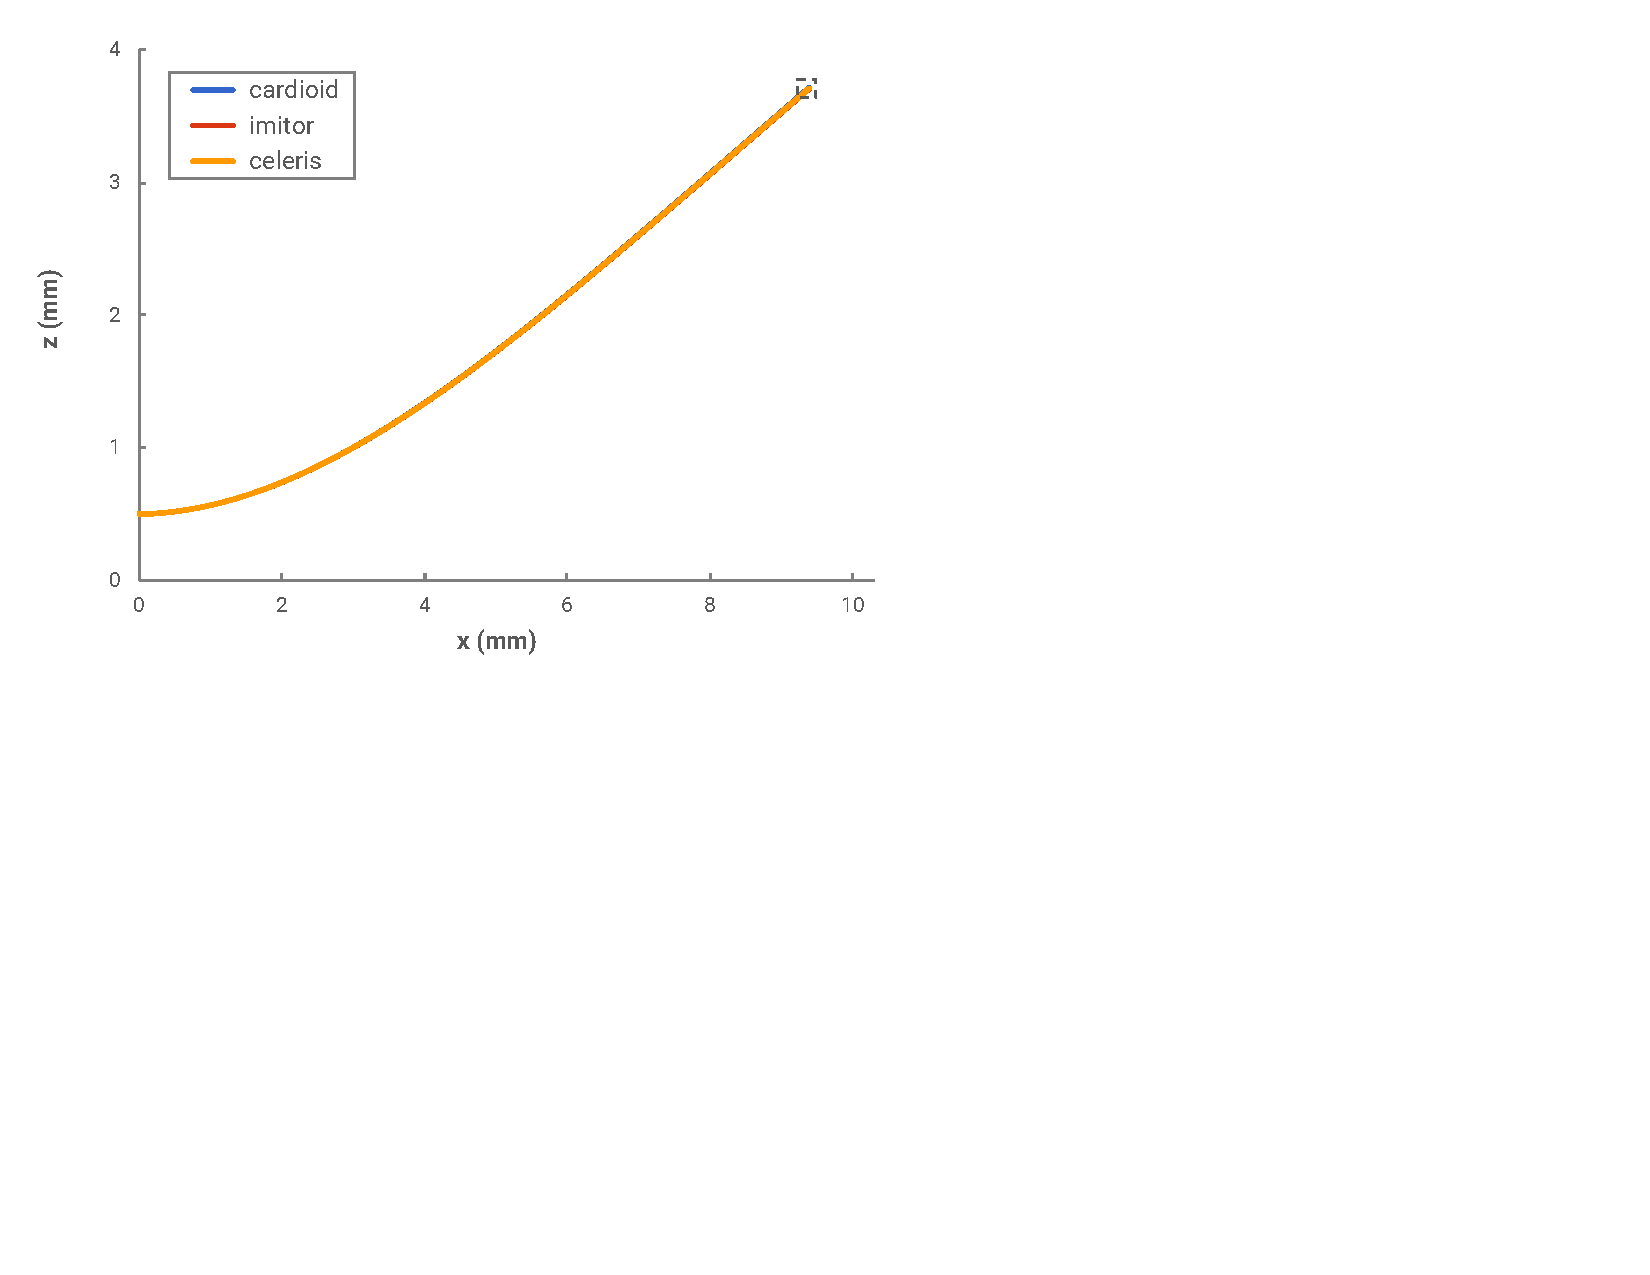
\includegraphics[scale=0.48]{media/5-verif/4-land1/land1-1.pdf}
\label{fig:land1-1}}		
\subfigure[]{%
		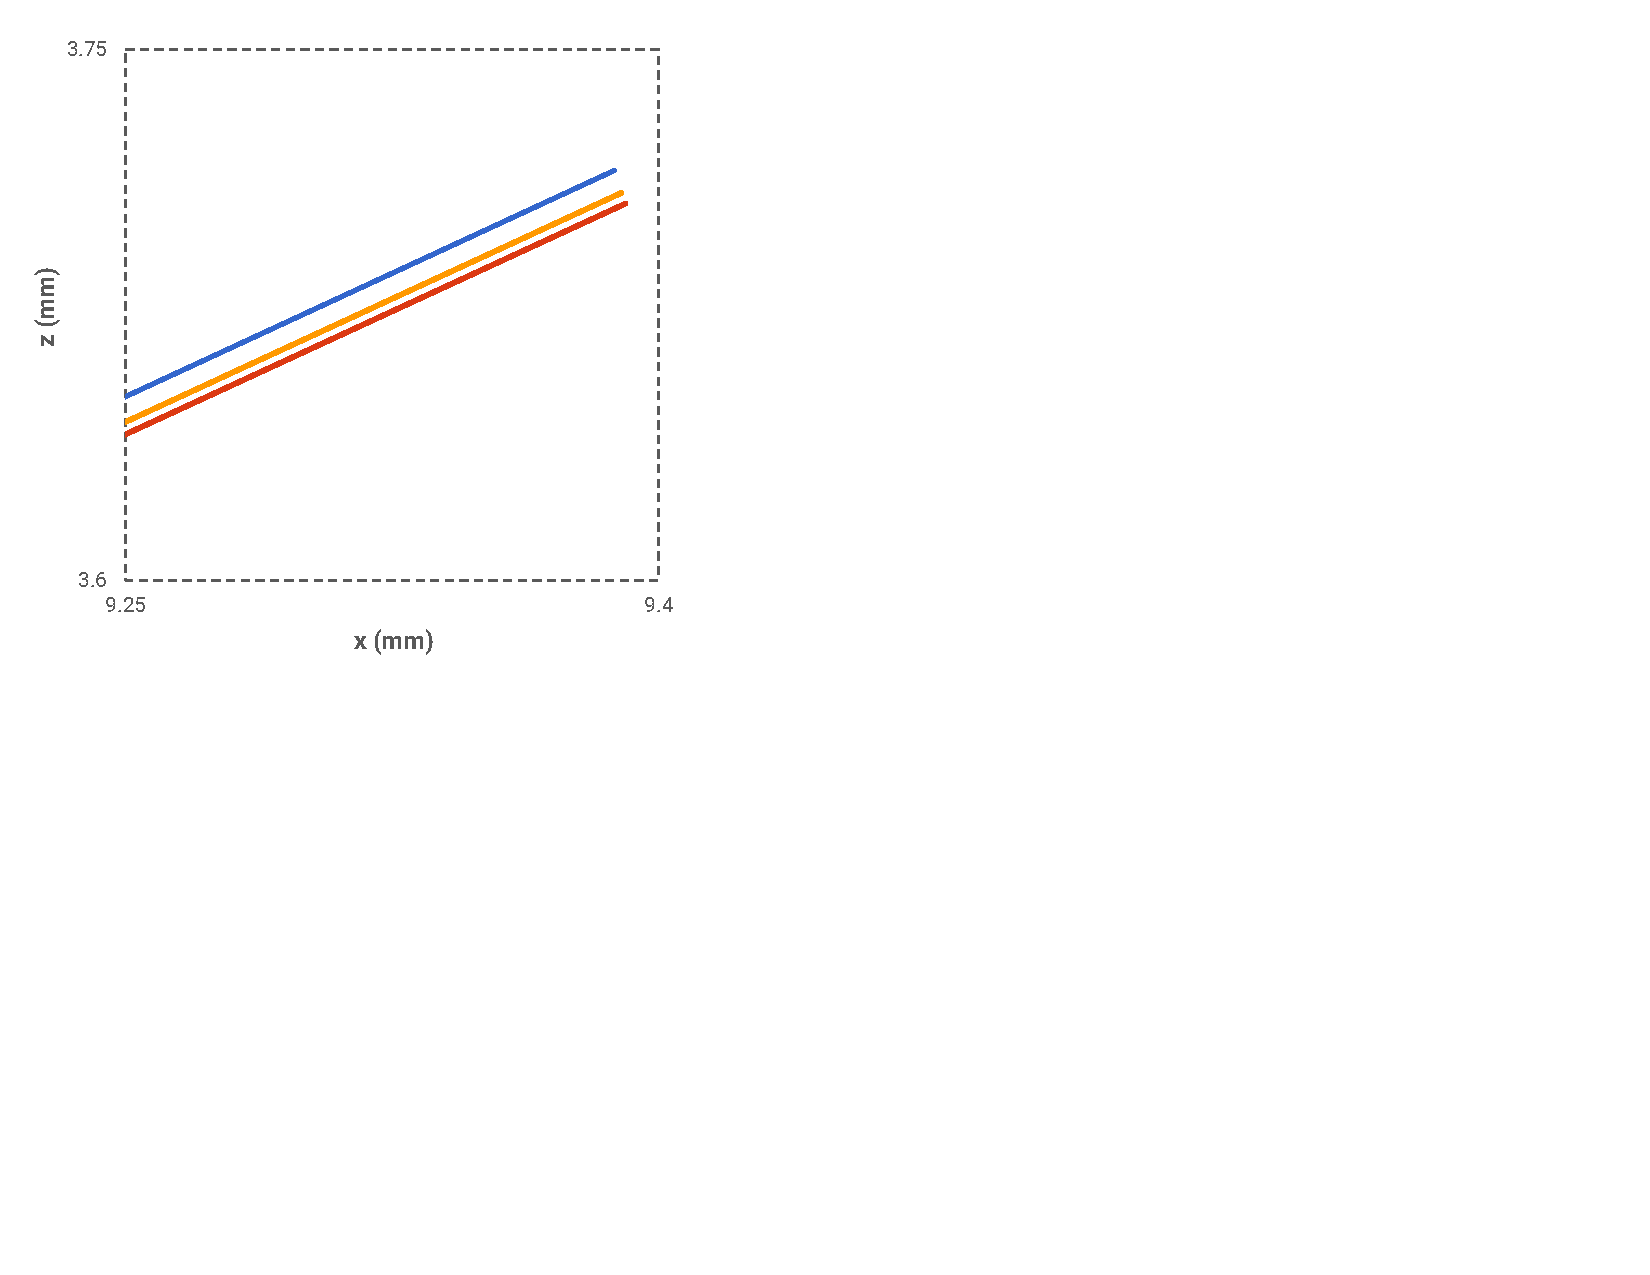
\includegraphics[scale=0.48]{media/5-verif/4-land1/land1-2.pdf}
\label{fig:land1-2}}	
\subfigure[]{%
		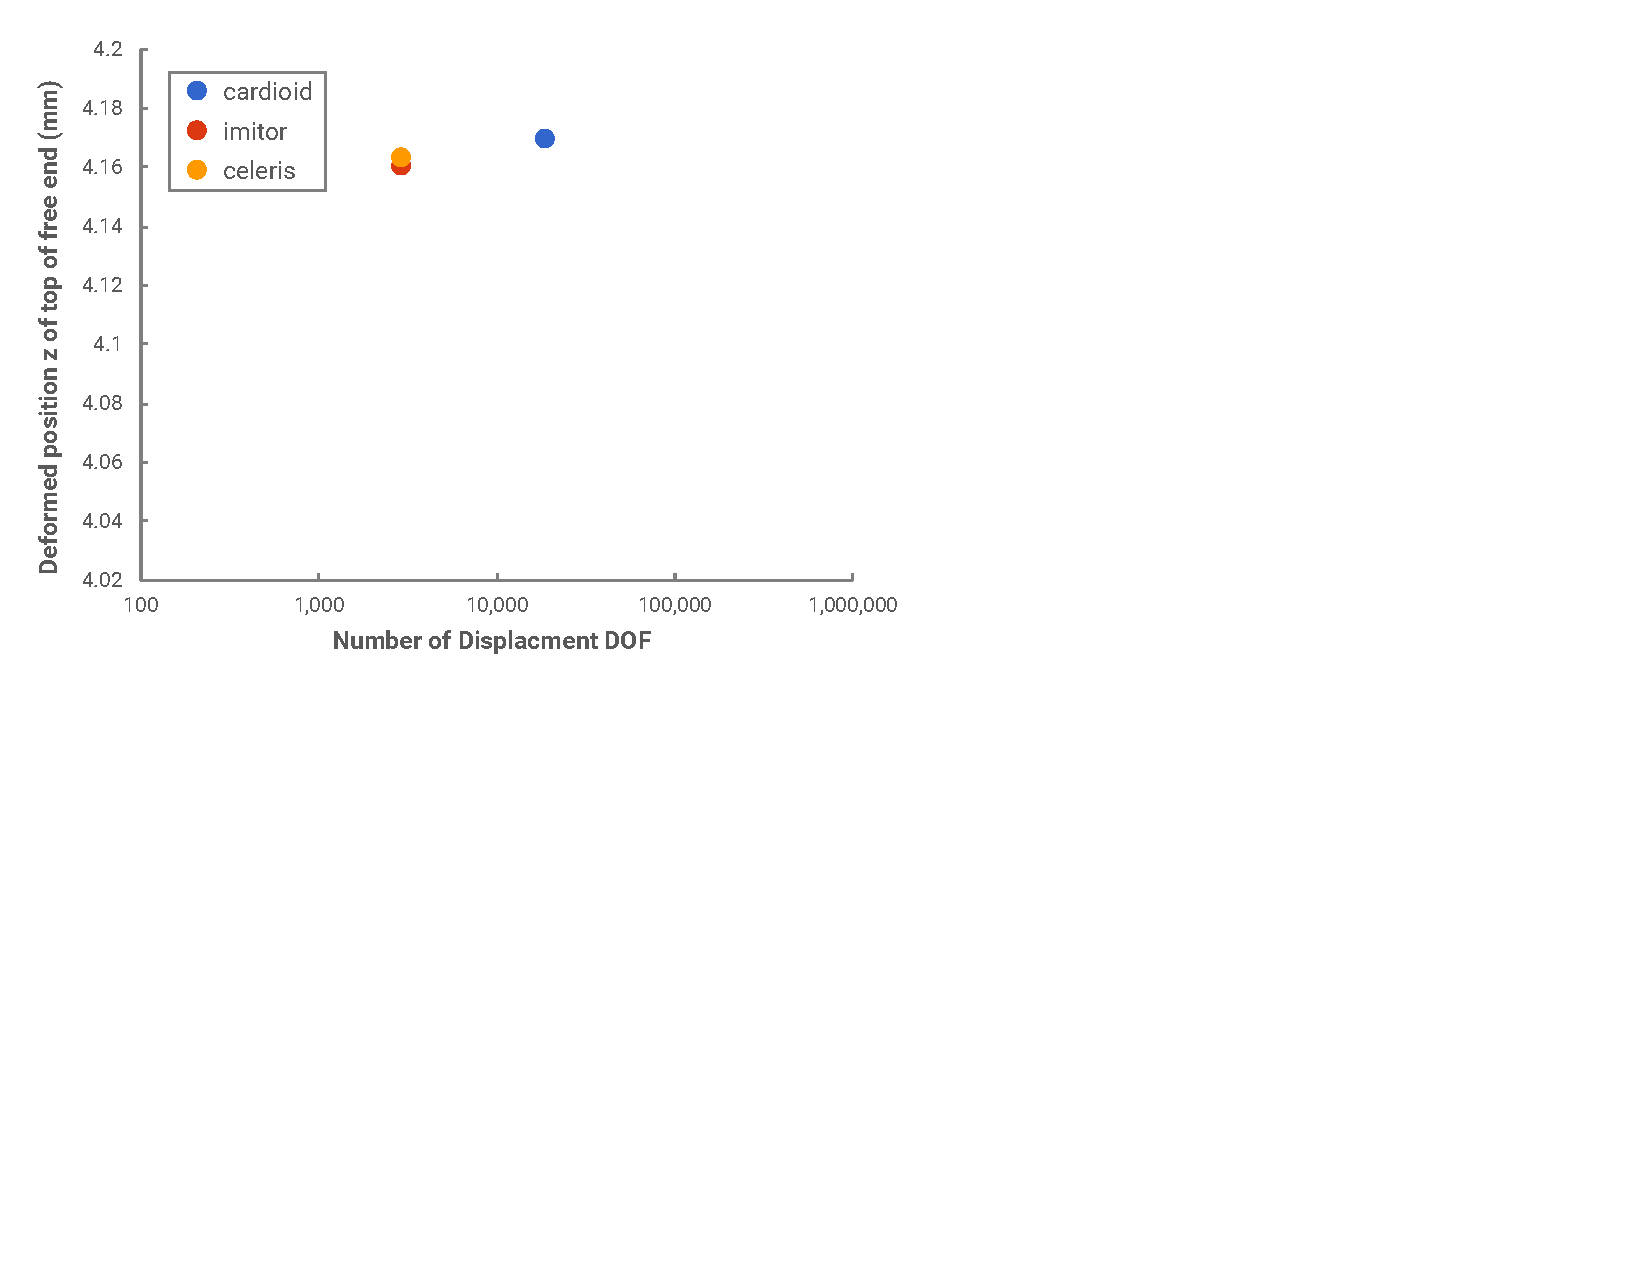
\includegraphics[scale=0.48]{media/5-verif/4-land1/land1-3.pdf}
\label{fig:land1-3}}			
%
\caption{Results for Land P1 verification problem: (a) Deformed position of midline, with (b) details for the free end of the beam. Panel (c) shows the deformed position of the point $\mathbf{X} = (10, 0.5, 1)$ for each of the simulation codes.}
\label{fig:land1}
\end{figure}


\begin{figure}[ht!]
\centering
\subfigure[]{%
		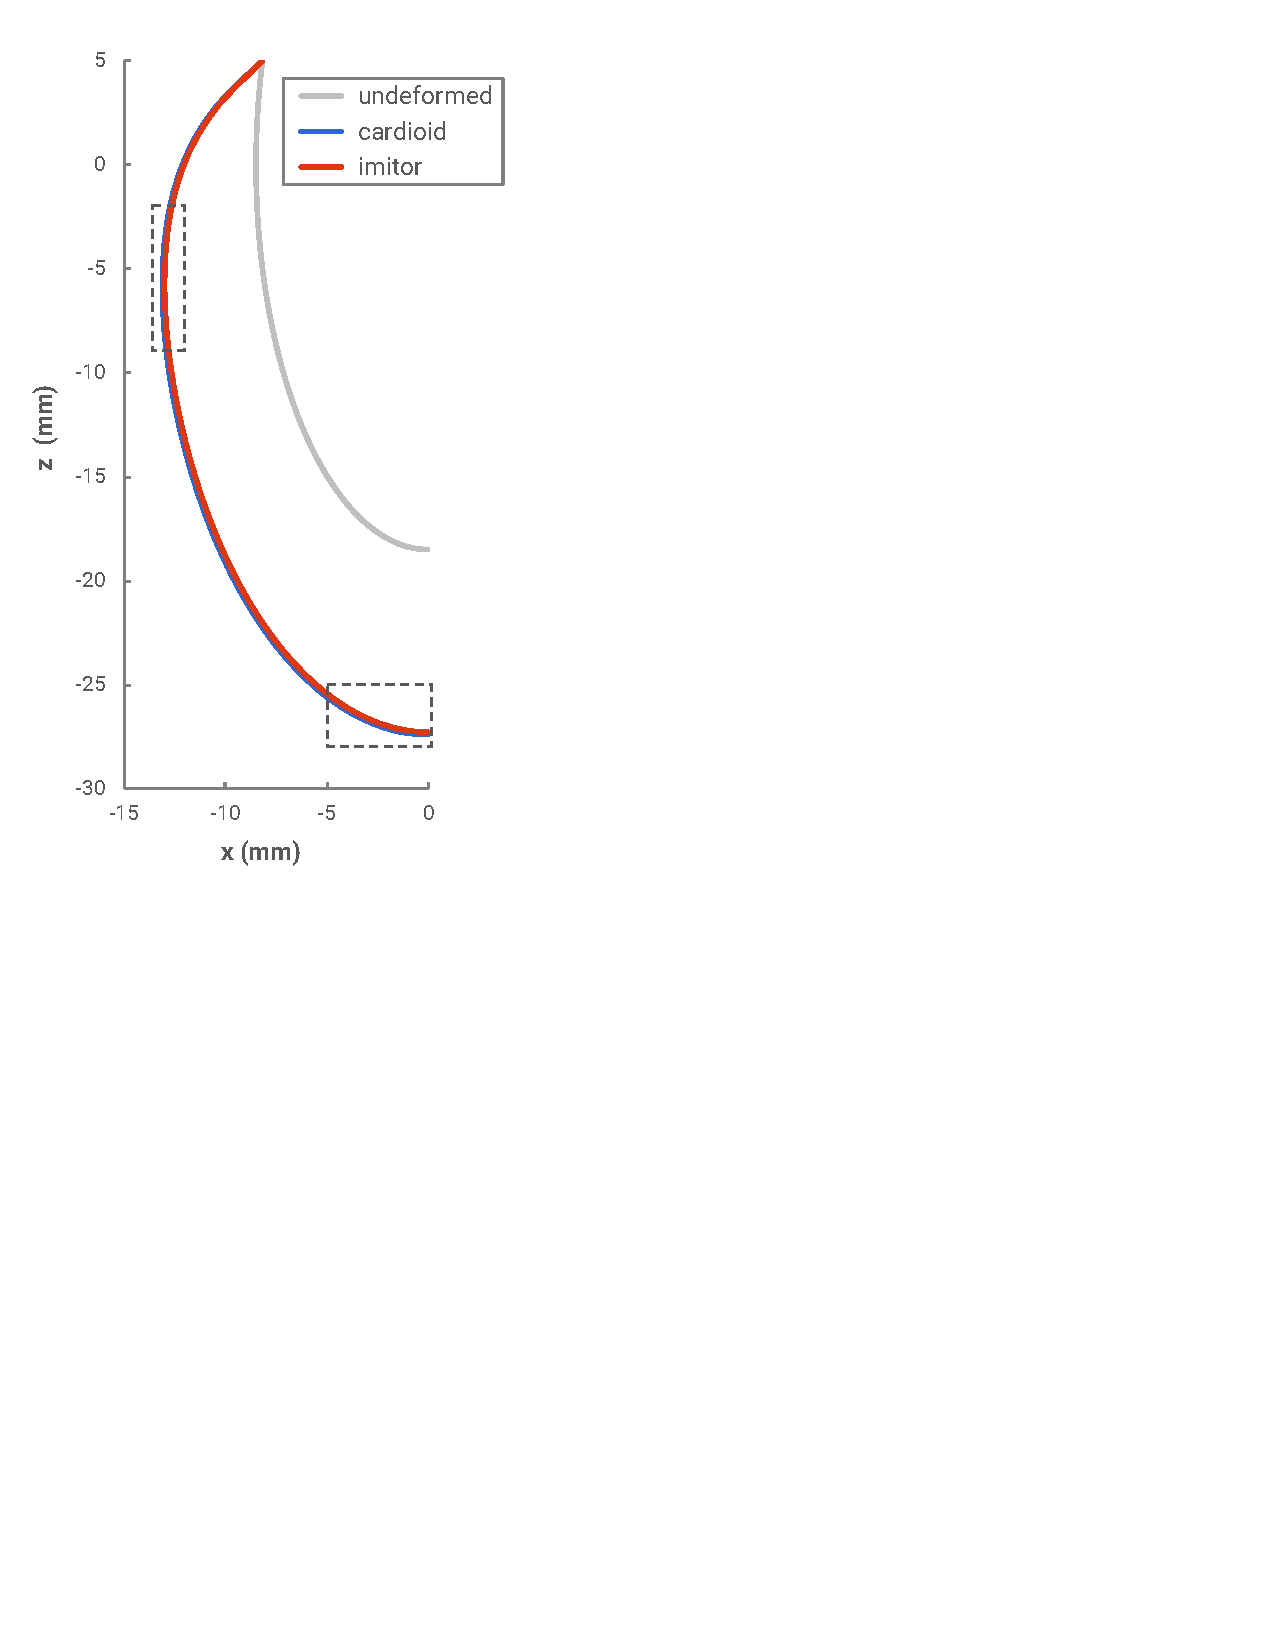
\includegraphics[scale=0.48]{media/5-verif/5-land2/land2-1.pdf}
\label{fig:land2-1}}		
\subfigure[]{%
		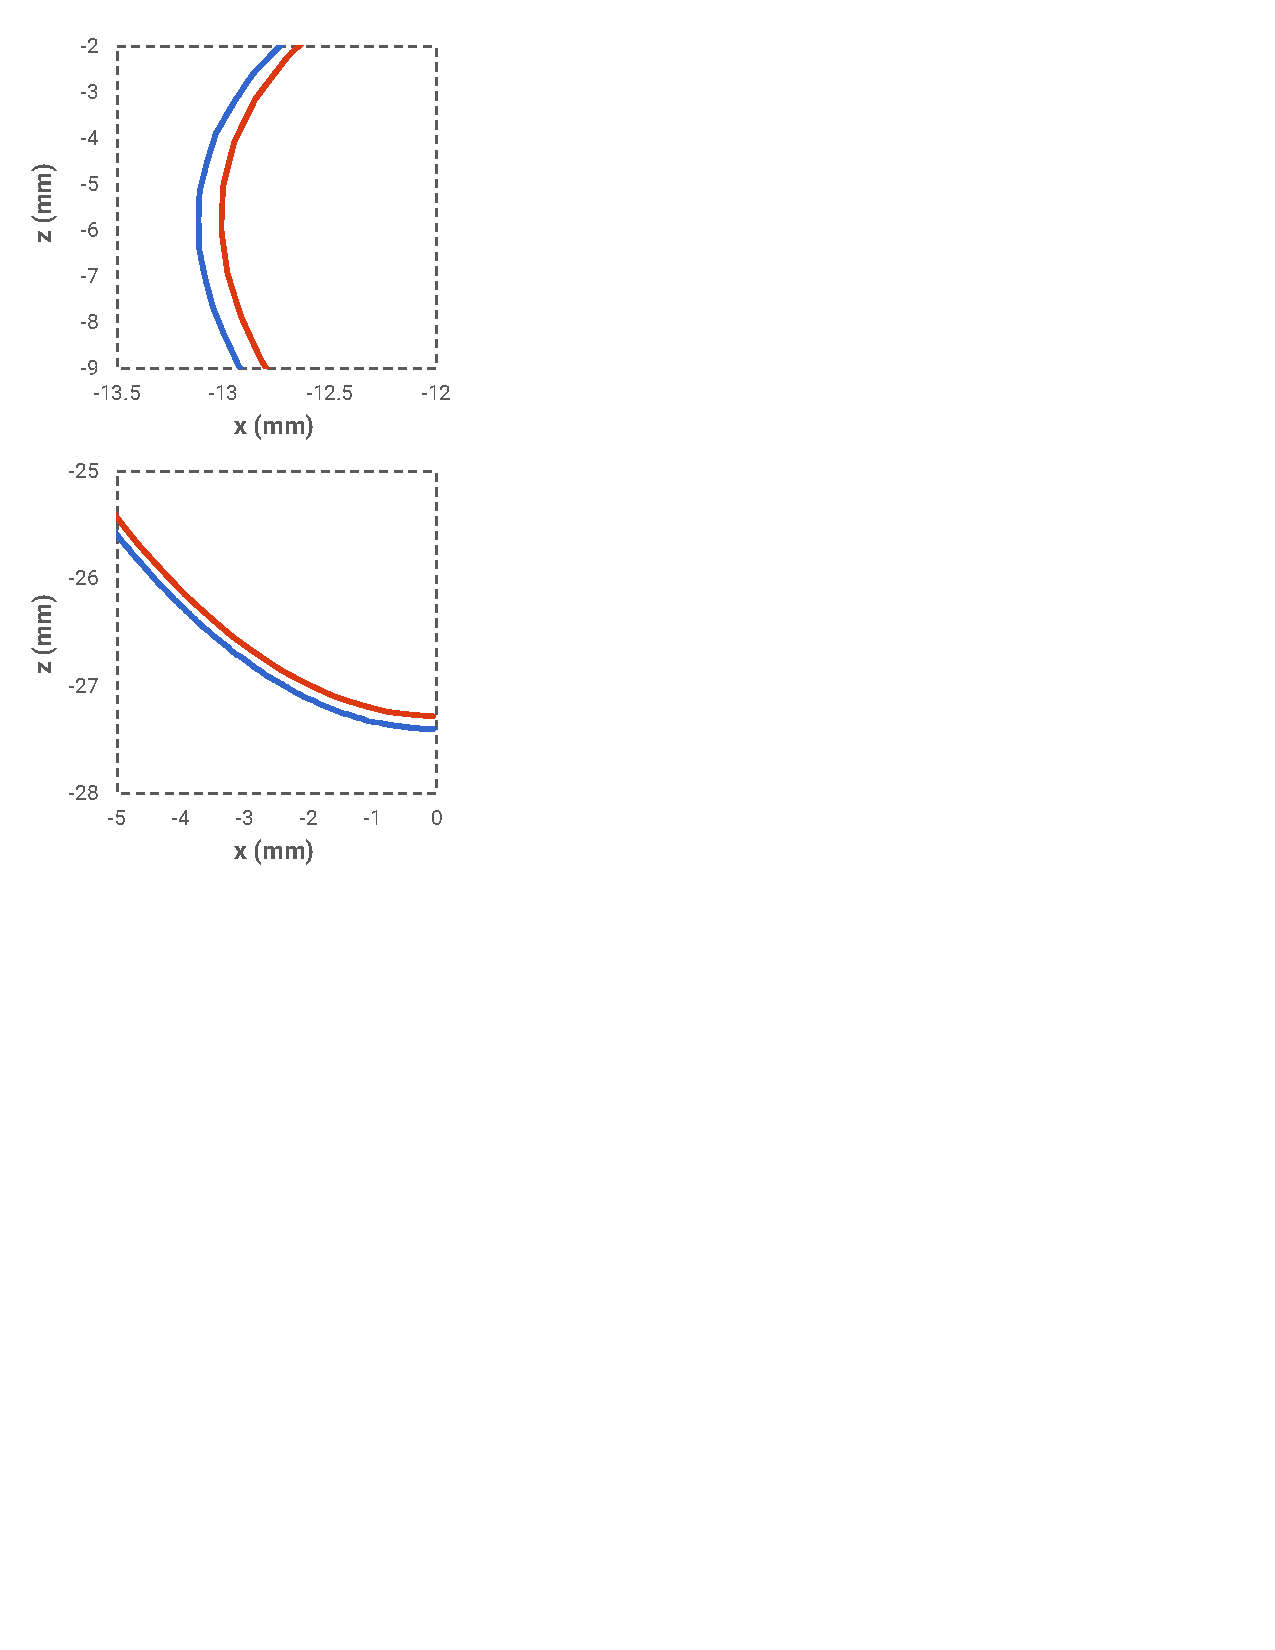
\includegraphics[scale=0.48]{media/5-verif/5-land2/land2-2.pdf}
\label{fig:land2-2}}	
\subfigure[]{%
		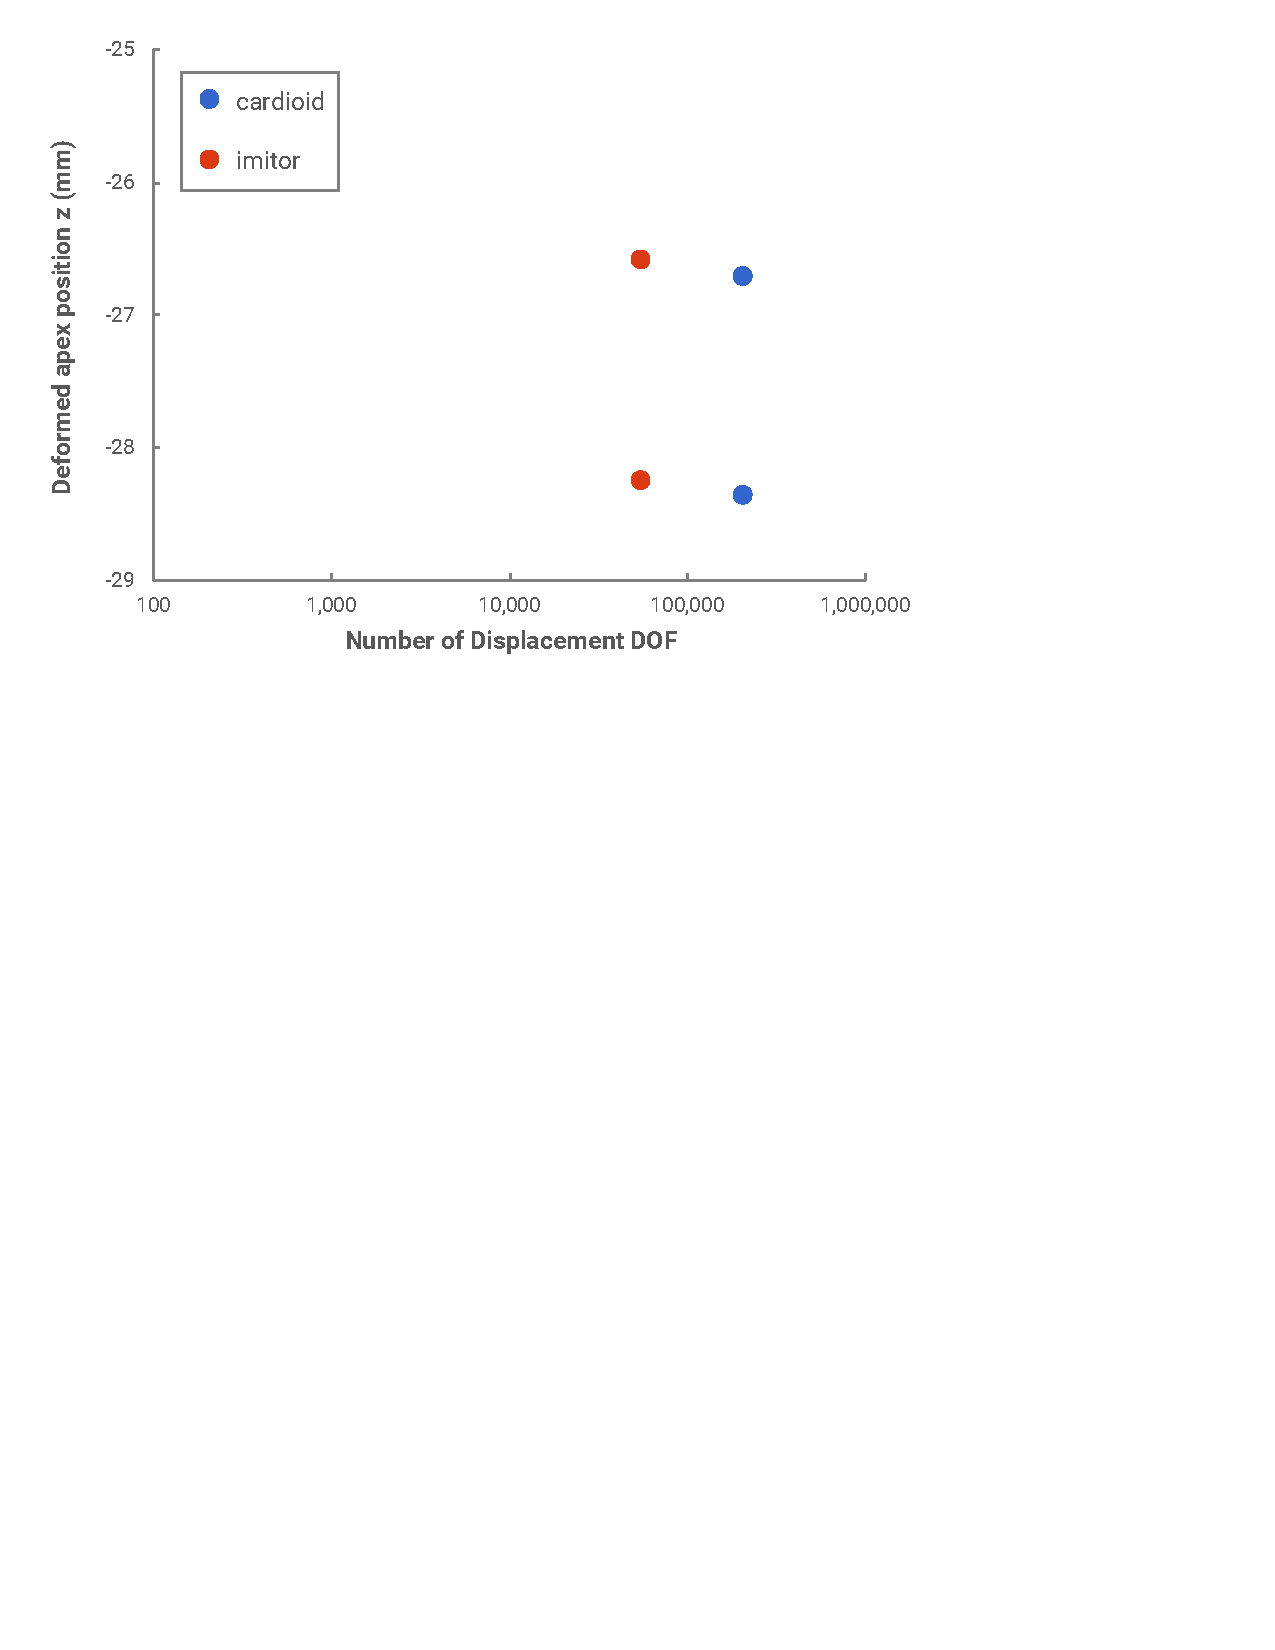
\includegraphics[scale=0.48]{media/5-verif/5-land2/land2-3.pdf}
\label{fig:land2-3}}			
%
\caption{Results for Land P2 verification problem: (a) Deformed position of middle of the ventricle wall, with (b) details at the inflection point (top right) and the apical region (bottom right). Panel (c) shows the deformed position of the apex at the endo- and epicardium for each of the simulation codes.}
\label{fig:land2}
\end{figure}

\begin{figure}[ht!]
\centering
\subfigure[]{%
		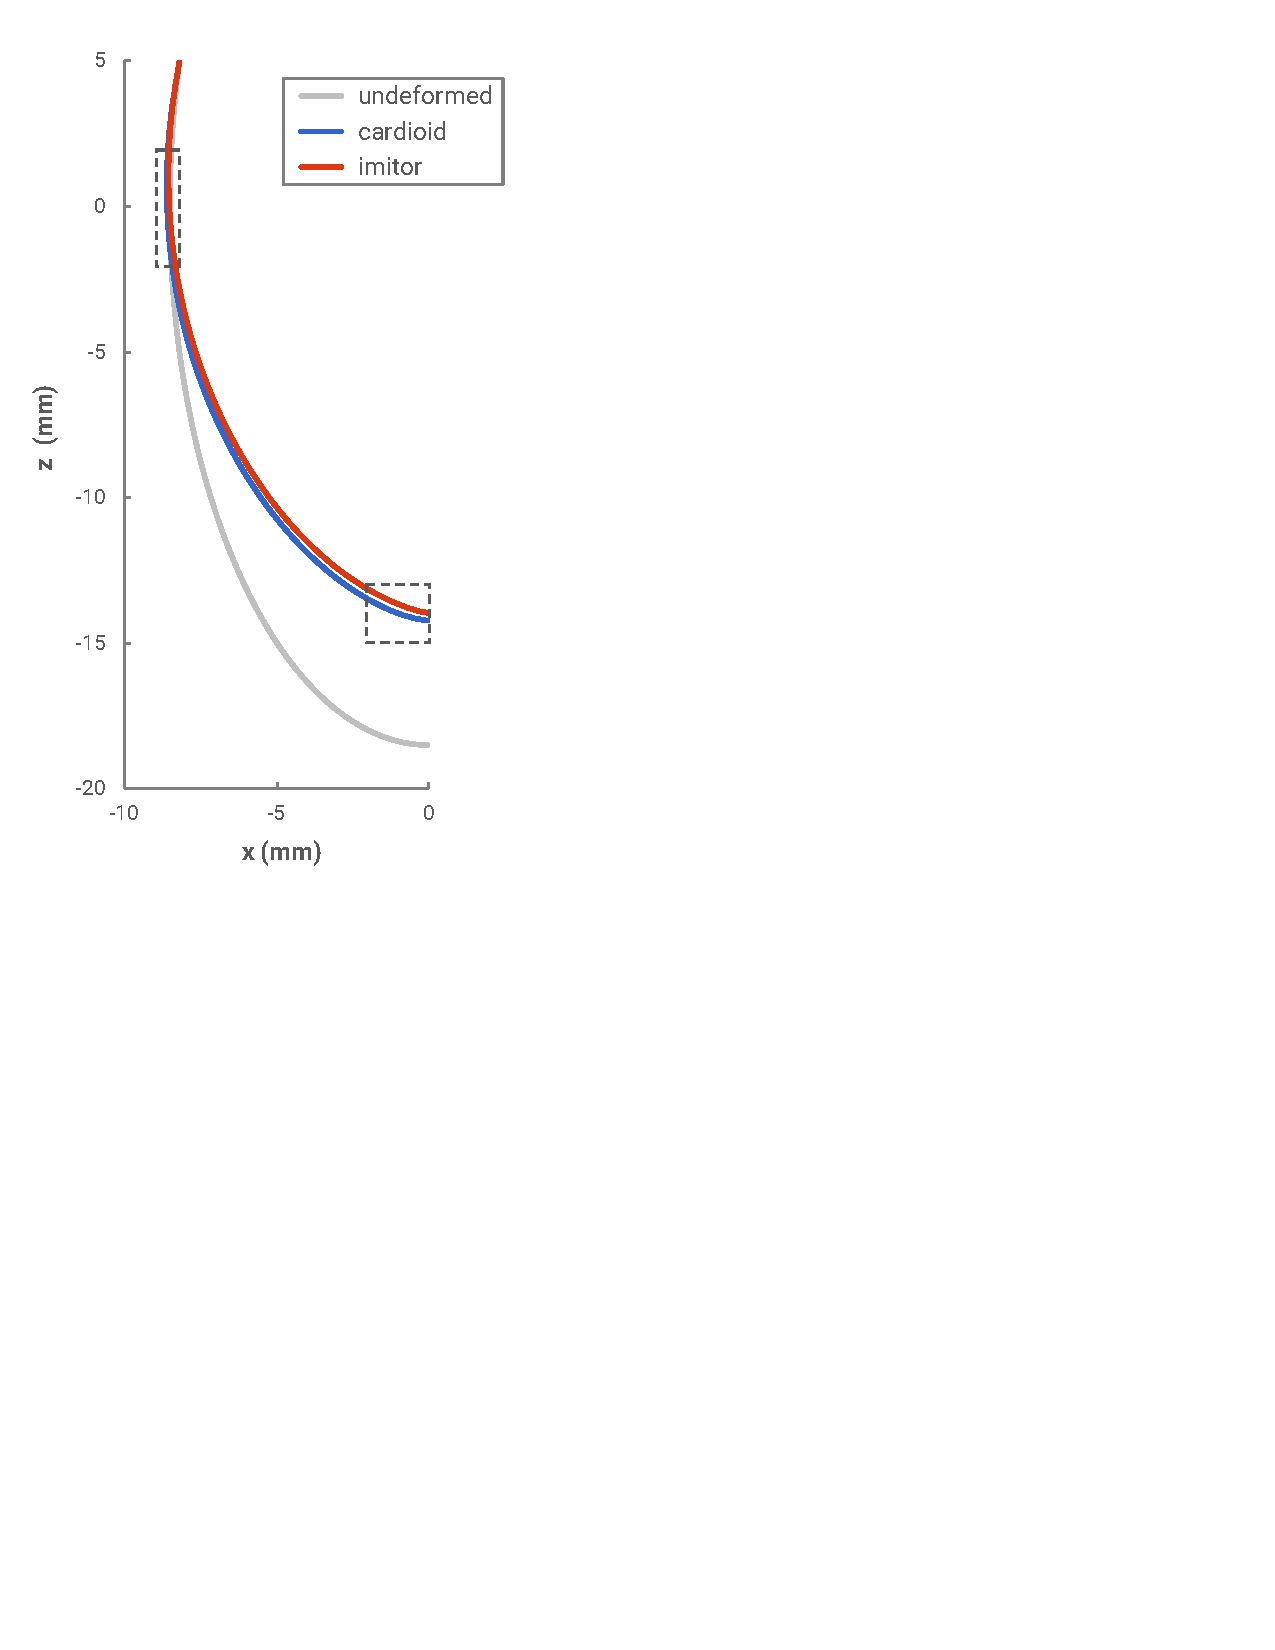
\includegraphics[scale=0.48]{media/5-verif/6-land3/land3-1.pdf}
\label{fig:land3-1}}		
\subfigure[]{%
		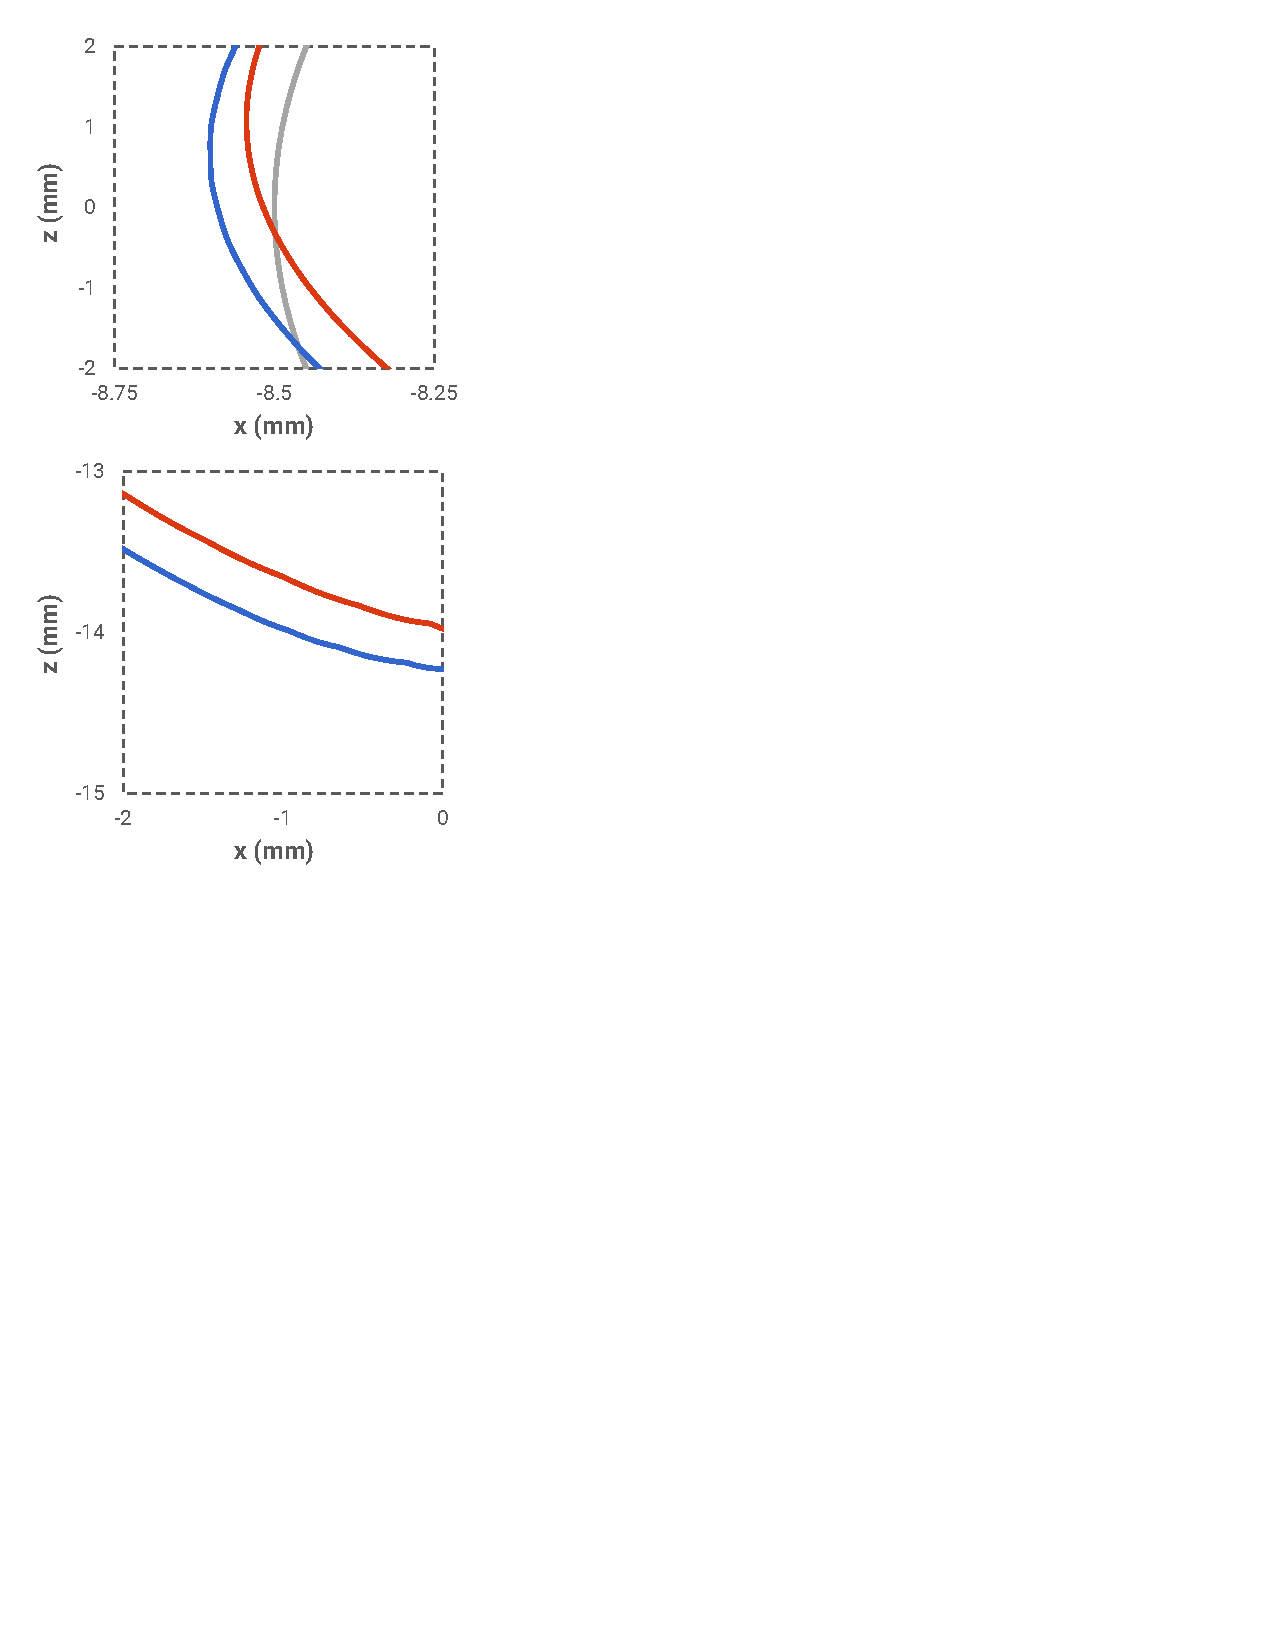
\includegraphics[scale=0.48]{media/5-verif/6-land3/land3-2.pdf}
\label{fig:land3-2}}	
%
\caption{Results for Land P3 verification problem: (a) Deformed position of middle of the ventricle wall, with (b) details at the inflection point (top right) and the apical region (bottom right).}
\label{fig:land3}
\end{figure}

\begin{figure}[ht!]
\centering
\subfigure[]{%
		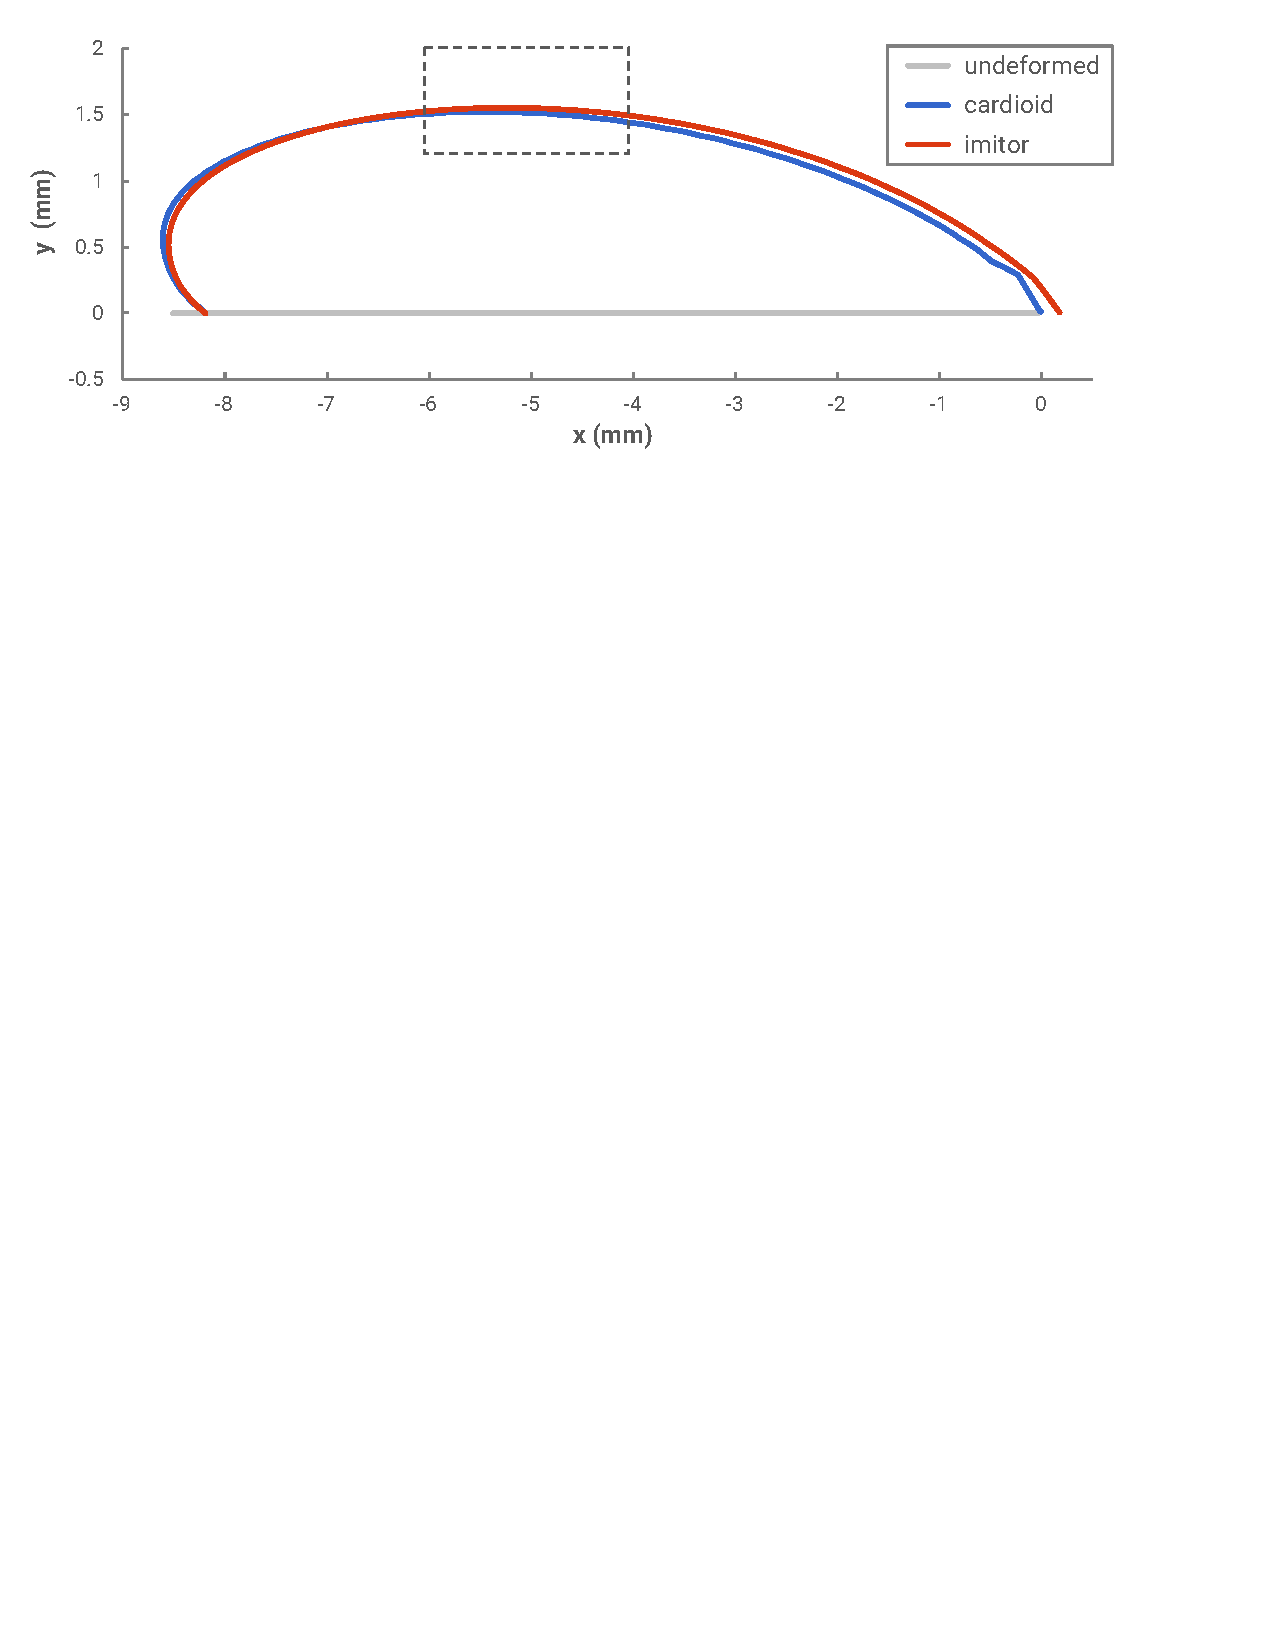
\includegraphics[scale=0.48]{media/5-verif/6-land3/land3-3.pdf}
\label{fig:land3.2-1}}		
\subfigure[]{%
		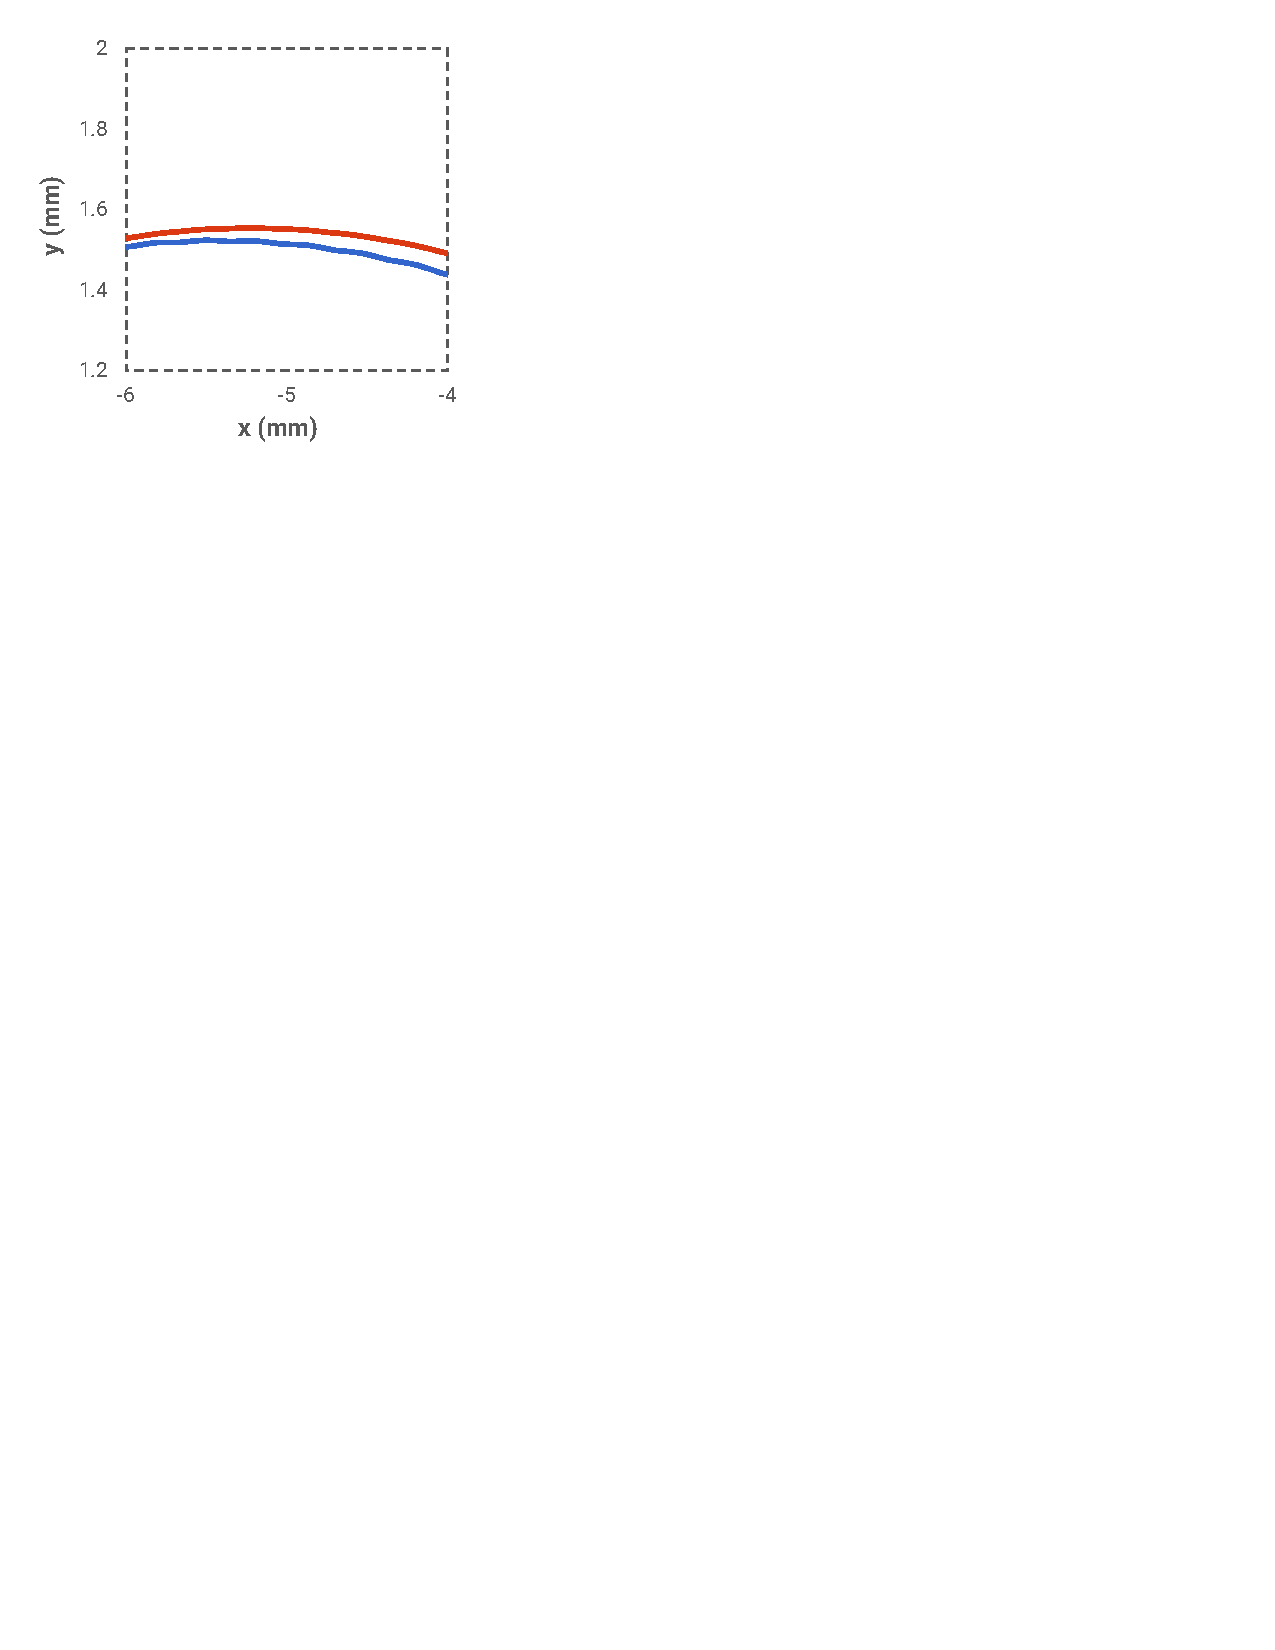
\includegraphics[scale=0.48]{media/5-verif/6-land3/land3-4.pdf}		
\label{fig:land3.2-2}}	
\subfigure[]{%
		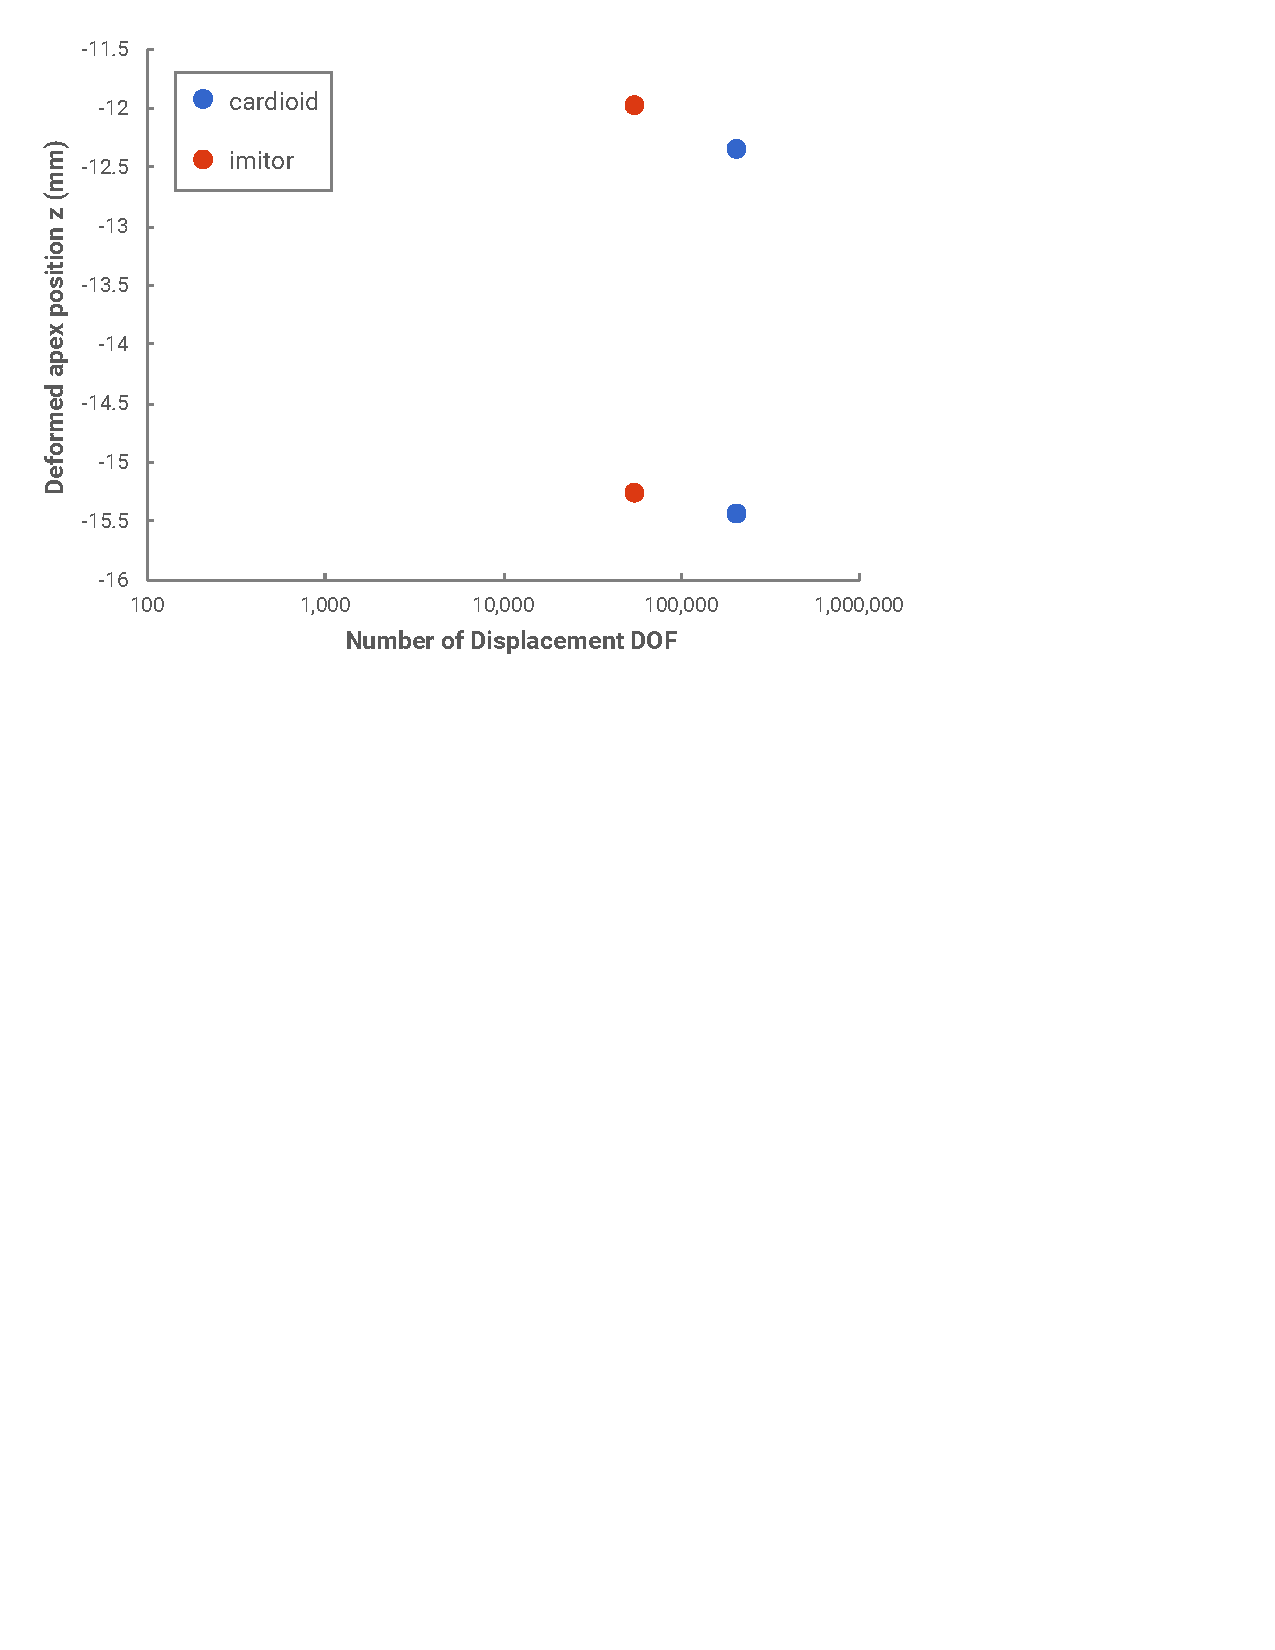
\includegraphics[scale=0.48]{media/5-verif/6-land3/land3-5.pdf}
\label{fig:land3.2-3}}			
	
%
\caption{Results for Land P3 verification problem: (a) The same deformed position of middle of the ventricle wall, shown in the $x-y$ plane, with (b) details at the inflection point. Panel (c) shows the deformed position of the apex at the endo- and epicardium for each of the simulation codes.}
\label{fig:land3.2}
\end{figure}


\begin{figure}[ht!]
\centering
\subfigure[]{%
		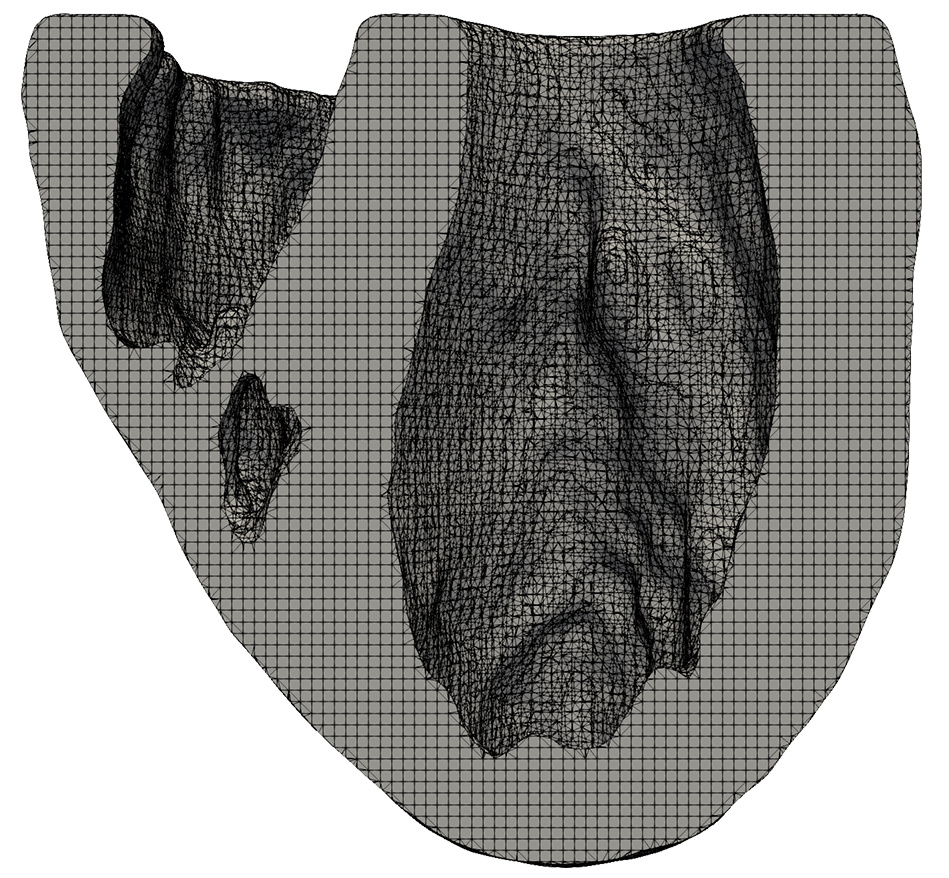
\includegraphics[scale=0.15]{media/3-celeris/8-celeris.png}
\label{fig:comp-1}}		
\subfigure[]{%
		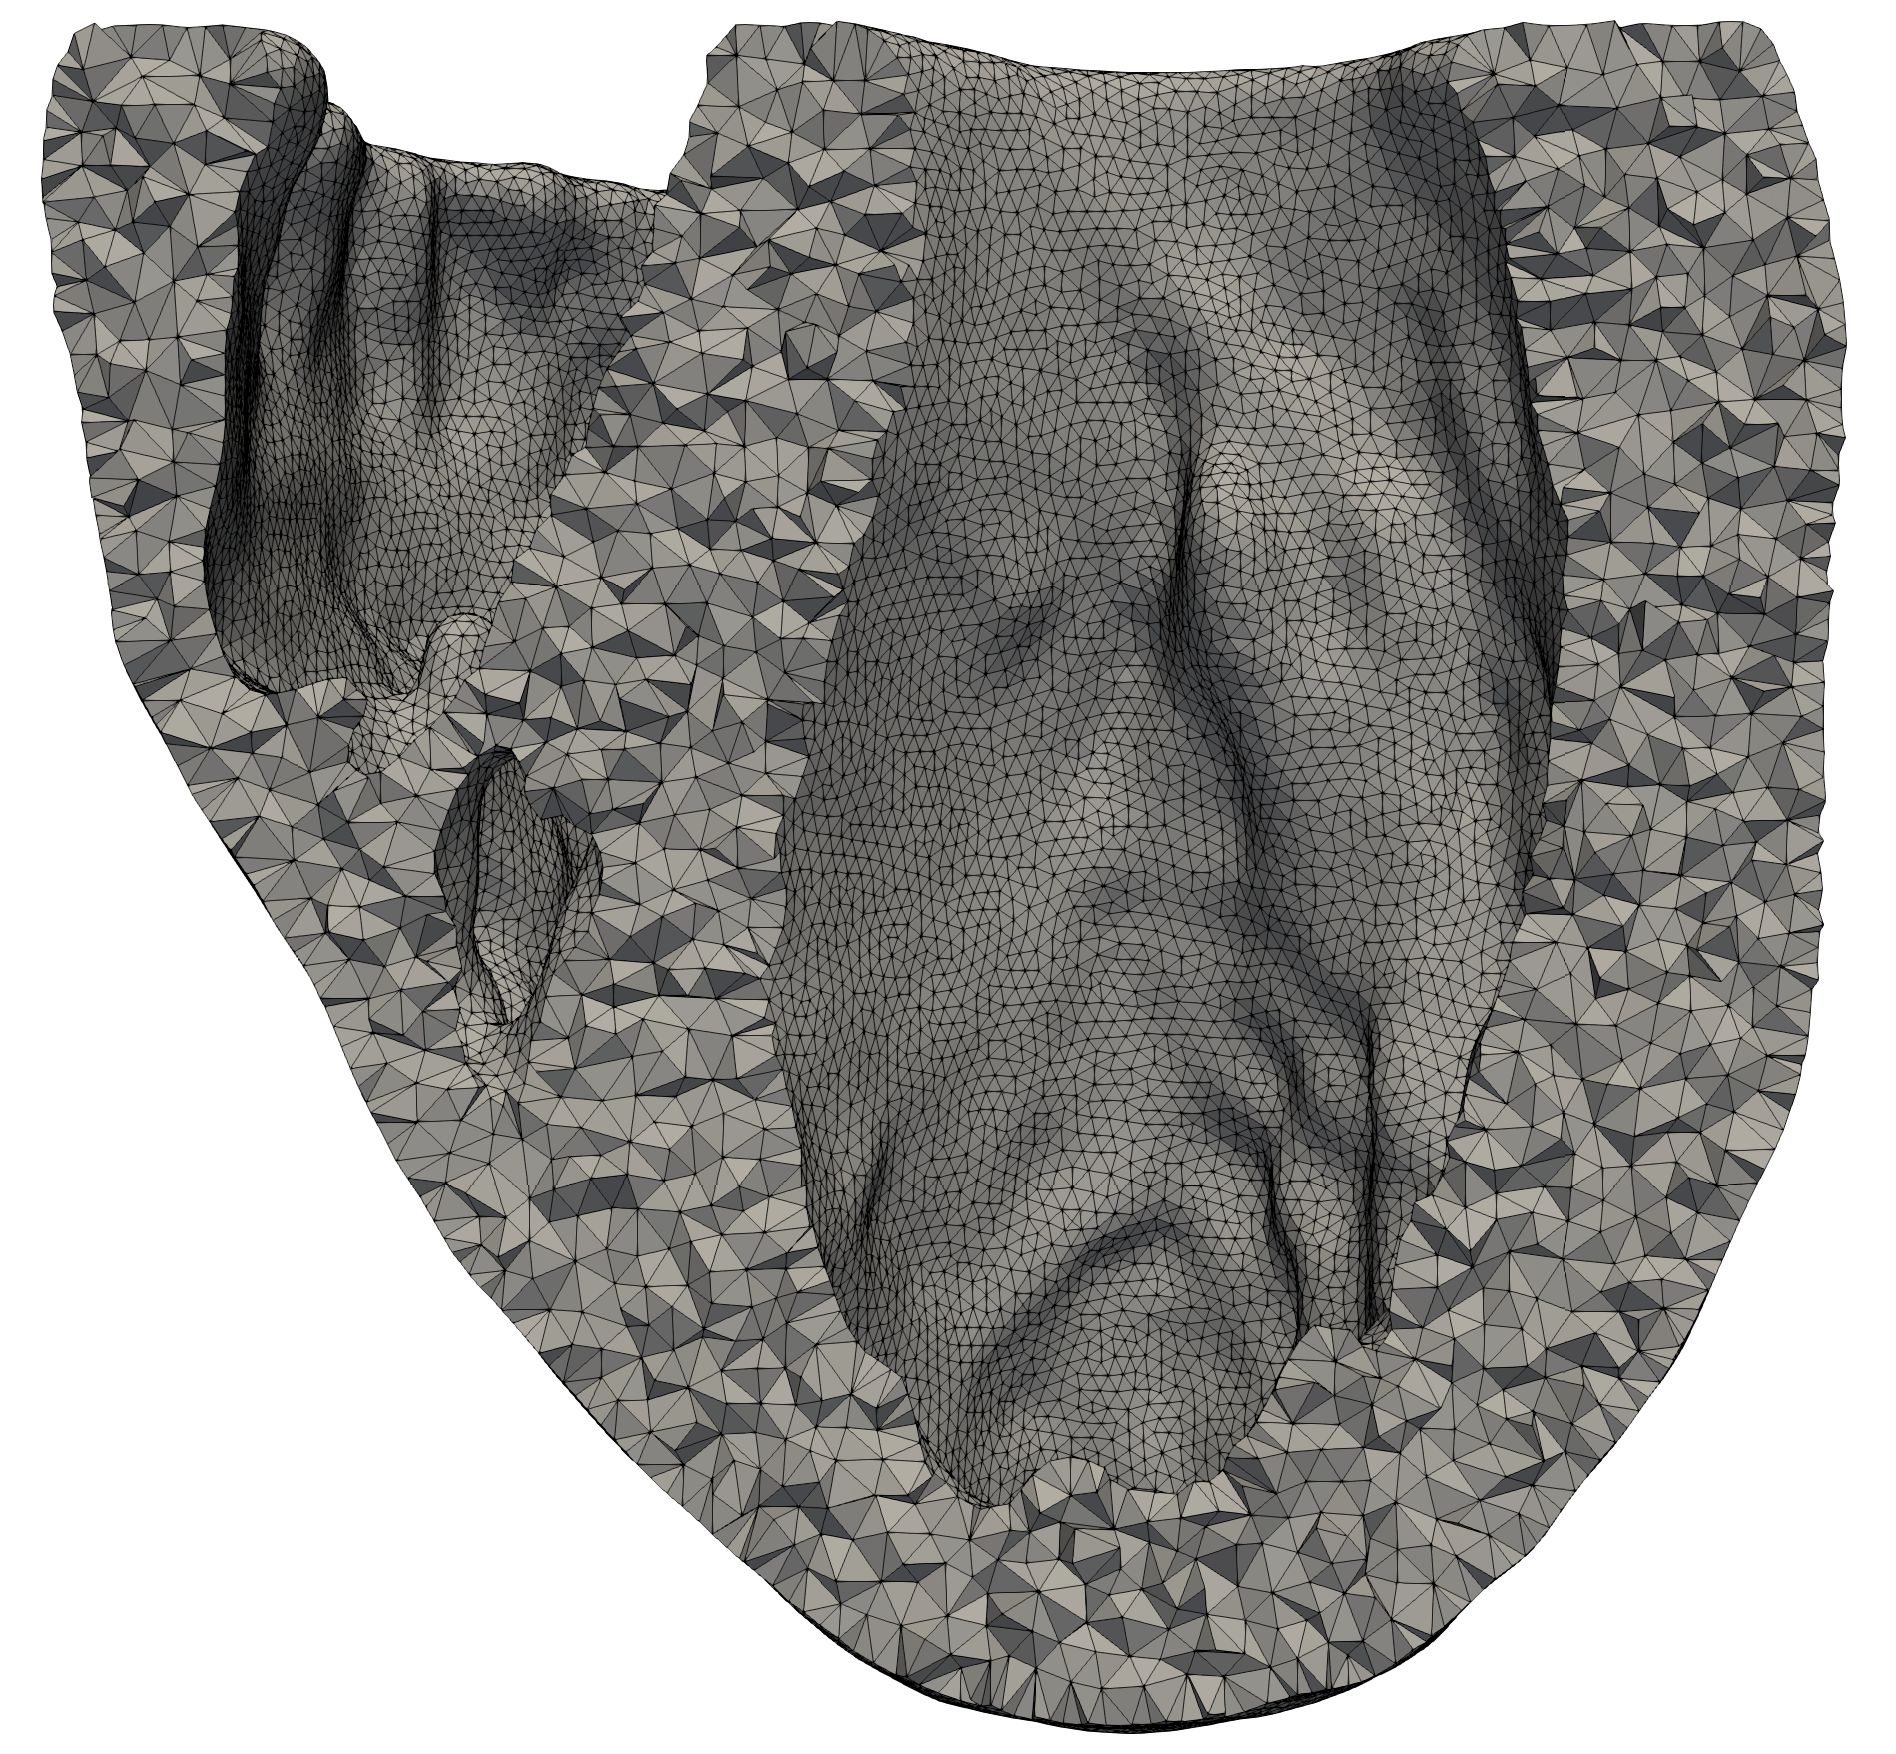
\includegraphics[scale=0.15]{media/3-celeris/9-cardioid.png}		
\label{fig:comp-2}}	
\subfigure[]{%
		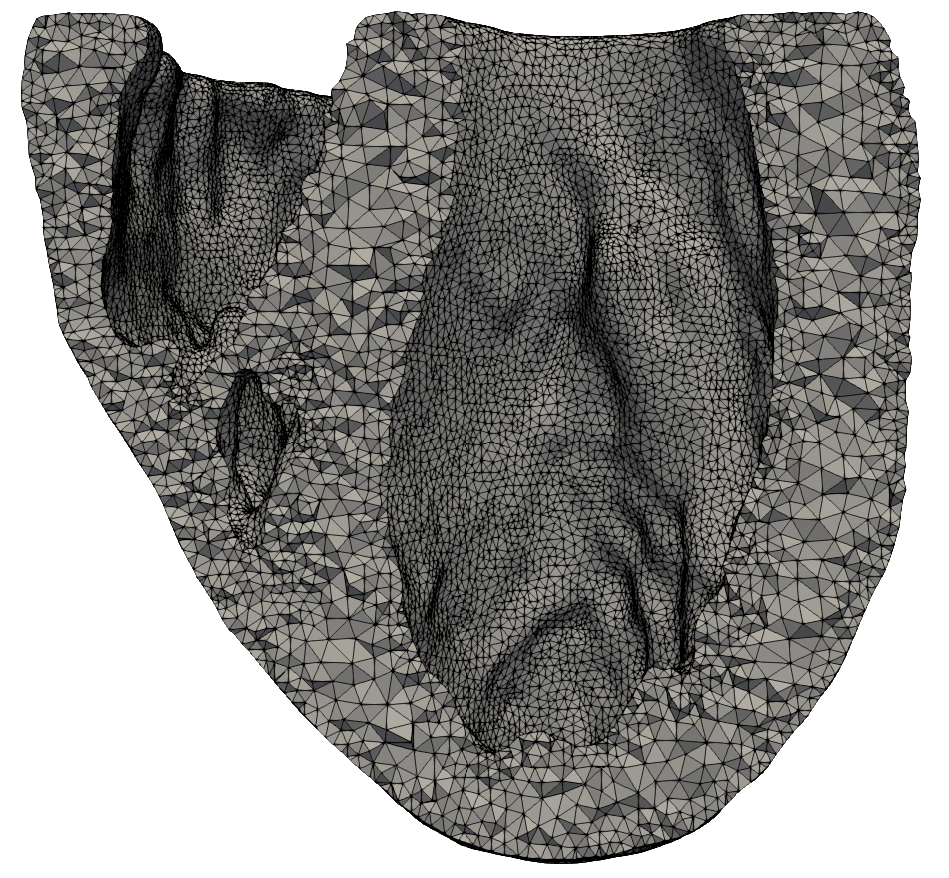
\includegraphics[scale=0.15]{media/3-celeris/10-simpleware.png}
\label{fig:comp-3}}			
	
%
\caption{Comparison of meshes: (a) linear polyhedral mesh from Celeris, (b) quadratic tetrahedral mesh from Tetgen, (c) and quadratic tetrahedral mesh from Simpleware.}
\label{fig:comp}
\end{figure}

{http://www.springer.com/us/book/9781441907295} \\
Cardioid science on saturday Youtube
$heart_papers$
papers Mark mentions in SOW

%%%%%%%%%%%%%%%%%%%%%%%%%%%%%%%%%%%%%%%%%%%%%%%
%%%%%%%%%%%%%%%%%%%%%%%%%%%%%%%%%%%%%%%%%%%%%%%
\section{Problem Description}
\label{Problem Description}

%%%%%%%%%%%%%%%%%%%%%%%%%%%%%%%%%%%%%%%%%%%%%%%
%%%%%%%%%%%%%%%%%%%%%%%%%%%%%%%%%%%%%%%%%%%%%%%
\section{Material Model}
\label{Material Model}

\subsection{Passive Stress}
\label{Passive Stress}

\subsection{Active Stress}
\label{Active Stress}

%%%%%%%%%%%%%%%%%%%%%%%%%%%%%%%%%%%%%%%%%%%%%%%
%%%%%%%%%%%%%%%%%%%%%%%%%%%%%%%%%%%%%%%%%%%%%%%
\section{Fiber Generation}
\label{Fiber Generation}

%%%%%%%%%%%%%%%%%%%%%%%%%%%%%%%%%%%%%%%%%%%%%%%
%%%%%%%%%%%%%%%%%%%%%%%%%%%%%%%%%%%%%%%%%%%%%%%
\section{Boundary Conditions}
\label{Boundary Conditions}

%%%%%%%%%%%%%%%%%%%%%%%%%%%%%%%%%%%%%%%%%%%%%%%
%%%%%%%%%%%%%%%%%%%%%%%%%%%%%%%%%%%%%%%%%%%%%%%
\section{Solver}
\label{Solver}

%%%%%%%%%%%%%%%%%%%%%%%%%%%%%%%%%%%%%%%%%%%%%%%
%%%%%%%%%%%%%%%%%%%%%%%%%%%%%%%%%%%%%%%%%%%%%%%
\section{Simulation Results}
\label{Simulation Results}
